\documentclass[11pt,twoside,openright]{book}
%%%%%%%%%%%%%%%%%%%%%%%%% PACKAGES %%%%%%%%%%%%%%%%%%%%%%%%%%
\usepackage[utf8]{inputenc}
\usepackage{textcomp}
\usepackage[english]{babel}
\usepackage{graphicx}
\usepackage{bm}
\usepackage{url}
\usepackage{rotating}
\usepackage{amsfonts}
\usepackage{verbatim}
\usepackage{amssymb}
\usepackage{pifont}
\usepackage{amsthm}
\usepackage{graphicx}
\usepackage{algorithmic}
\usepackage{algorithm}
\usepackage{listings}
\usepackage{cite}
\usepackage{fix2col}
\usepackage{color}
\usepackage{geometry}
\usepackage{longtable}
\usepackage{chngpage}
\usepackage{amsmath}
\usepackage{booktabs}
\usepackage{subfig}
\usepackage{pifont}
\usepackage{multirow}
\usepackage{lscape}
\usepackage{xspace}
\usepackage{mdwtab}
\usepackage{float}
%\usepackage{mathptmx}        % selects Times Roman as basic font
\usepackage{helvet}          % selects Helvetica as sans-serif font
\usepackage{courier}         % selects Courier as typewriter font
\usepackage{type1cm}         % activate if the above 3 fonts are not available on your system
\usepackage{makeidx}         % allows index generation
\usepackage{graphicx}        % standard LaTeX graphics tool when including figure files
\usepackage{multicol}        % used for the two-column index
\usepackage[bottom]{footmisc}% places footnotes at page bottom
%\usepackage[hidelinks, breaklinks]{hyperref}
%\usepackage{epsfig}
\usepackage{graphicx}
\usepackage{rotating}
\usepackage{amsmath}
\usepackage{amssymb}
\usepackage{multirow}
\usepackage{array}
\usepackage{longtable}
\usepackage{tikz}
\usepackage{verbatim}
\usepackage{pdfpages}
\usepackage{hyperref}                 % Active hyperlink
\usepackage[hyperpageref]{backref}    % Add 'backlink' page number at the end of each item in the bibliography BibTeX
\hypersetup{
    %Since 2011-02-05 (hyperref version 6.82a), you can use the hidelinks option to achieve the same result
    colorlinks=false,
    pdfborder={0 0 0},
}

%\usetikzlibrary{fit,arrows,matrix,calc,positioning,shapes,backgrounds}
%\usepackage{algpseudocode}
%%%%%%%%%%%%%%%%%%%%%%%%% INCLUDES %%%%%%%%%%%%%%%%%%%%%%%%%%
%\newcommand{\RR}{\rm I\hspace{-0.55ex}R}
%\newcommand{\NN}{\rm I\hspace{-0.55ex}N}
%\renewcommand{\baselinestretch}{1.0}

% New theorems
\theoremstyle{definition}
\newtheorem{definition}{Definition}[chapter]
\newtheorem{theorem}{Theorem}[section]

\theoremstyle{plain}
\newtheorem{lemma}[theorem]{Lemma}
\newtheorem{proposition}[theorem]{Proposition}
\newtheorem{corollary}[theorem]{Corollary}

% Own commands
\newcommand{\ie}{{\em i.e.~}}
\newcommand{\mI}{\mathbf{I}}
\newcommand{\mone}{\mathbf{1}}
\newcommand{\eg}{{\em e.g.~}}
\newcommand{\etal}{{\em et al.}}
\newcommand{\vs}{{\em vs}}
\newcommand{\fig}[1]{Figure \ref{#1}}
\newcommand{\eq}[1]{Eqn. \ref{#1}}
\newcommand{\sect}[1]{Section \ref{#1}}
\newcommand{\ch}[1]{Chapter \ref{#1}}
\newcommand{\app}[1]{Appendix \ref{#1}}
\newcommand{\dataset}{{\cal D}}
\newcommand{\fracpartial}[2]{\frac{\partial #1}{\partial  #2}}
\newcommand{\mycaption}[1]{\caption{ \protect{{\small\sf #1}} }}
\newcommand{\mcomma}{, \allowbreak}
\newcommand{\cmark}{\ding{51}}
\newcommand{\xmark}{\ding{55}}

% Own Operators
\DeclareMathOperator*{\argmax}{arg\,max}


% PAMI
\newcommand{\D}{\delta}
\newcommand{\fspc}{\Omega}
\newcommand{\lspc}{\mathcal{Y}}
\newcommand{\sspc}{\mathcal{S}}

\newcommand{\desc}{\mathbf{D}}
\newcommand{\oracle}{{\mathcal{O}}}
\newcommand{\vx}{\mathbf{x}}
\newcommand{\sample}{\mathbf{s}}
\newcommand{\lab}{y}

\newcommand{\ActPos}{Act$+$}
\newcommand{\ActNeg}{Act$-$}
\newcommand{\ActPosNeg}{Act$\pm$}
\newcommand{\ActGT}{Act$\sim$}

\newcommand{\pD}{p(\sample,\lab)}
\newcommand{\pDvx}{p(\vx,\lab)}

\newcommand{\training}{tr}
\newcommand{\testing}{tt}

\newcommand{\vxTr}{\vx^{\training}}
\newcommand{\sampleTr}{\sample^{\training}}
\newcommand{\labTr}{\lab^{\training}}

\newcommand{\vxTt}{\vx^{\testing}}
\newcommand{\sampleTt}{\sample^{\testing}}
\newcommand{\labTt}{\lab^{\testing}}

\newcommand{\TS}{\mathcal{T}}
\newcommand{\TrS}{\TS^{\training}}
\newcommand{\TrSPos}{\TS^{\training +}}
\newcommand{\TrSNeg}{\TS^{\training -}}
\newcommand{\TtS}{\TS^{\testing}}

\newcommand{\clsf}{\mathrm{C}}
\newcommand{\detect}{\mathrm{D}}

\newcommand{\Ds}{\D_s}
\newcommand{\Dt}{\D_t}
\newcommand{\pDs}{p_{s}(\sample,\lab)}
\newcommand{\pDt}{p_{t}(\sample,\lab)}
\newcommand{\pDvxs}{p_{s}(\vx,\lab)}
\newcommand{\pDvxt}{p_{t}(\vx,\lab)}
\newcommand{\TrSs}{\TS^{\training, s}}
\newcommand{\TrSt}{\TS^{\training, t}}
\newcommand{\TrSPoss}{\TS^{\training +, s}}
\newcommand{\TrSPost}{\TS^{\training +, t}}
\newcommand{\TtSt}{\TS^{\testing, t}}

\newcommand{\Daimler}{{\mathcal{D}}}
\newcommand{\INRIA}{{\mathcal{I}}}
\newcommand{\Virtual}{{\mathcal{V}}}

\newcommand{\SX}{\mathcal{X}}
\newcommand{\SR}{\mathcal{R}}
\newcommand{\TrSX}{\TrS_{\SX}}
\newcommand{\TrSR}{\TrS_{\SR}}
\newcommand{\TtSR}{\TtS_{\SR}}

\newcommand{\TrSVirtual}{\TrS_{\Virtual}}
\newcommand{\TrSINRIA}{\TrS_{\INRIA}}
\newcommand{\TrSDaimler}{\TrS_{\Daimler}}
\newcommand{\TtSINRIA}{\TtS_{\mathcal{I}}}
\newcommand{\TtSDaimler}{\TtS_{\Daimler}}

\newcommand{\TrSVirtualPos}{\TrSPos_{\Virtual}}
\newcommand{\TrSINRIAPos}{\TrSPos_{\INRIA}}
\newcommand{\TrSDaimlerPos}{\TrSPos_{\Daimler}}
\newcommand{\TrSXPos}{\TrSPos_{\SX}}
\newcommand{\TrSRPos}{\TrSPos_{\SR}}

\newcommand{\TrSVirtualNeg}{\TrSNeg_{\Virtual}}
\newcommand{\TrSINRIANeg}{\TrSNeg_{\INRIA}}
\newcommand{\TrSDaimlerNeg}{\TrSNeg_{\Daimler}}
\newcommand{\TrSXNeg}{\TrSNeg_{\SX}}
\newcommand{\TrSRNeg}{\TrSNeg_{\SR}}

\newcommand{\TrTt}[2]{\{#1,#2\}}

\newcommand{\Source}{\Virtual}
\newcommand{\Target}{\SR}

\newcommand{\TrSTarget}{\TrS_{\Target}}
\newcommand{\TtSTarget}{\TtS_{\Target}}

\newcommand{\ImSet}{\Im}
\newcommand{\TrIS}{\ImSet^{\training}}
\newcommand{\TrISPos}{\ImSet^{\training +}}
\newcommand{\TrISNeg}{\ImSet^{\training -}}
\newcommand{\TtIS}{\ImSet^{\testing}}

\newcommand{\TrISSourcePos}{\TrISPos_{\Virtual}}
\newcommand{\TrISSourceNeg}{\TrISNeg_{\Virtual}}
\newcommand{\TrISSource}{\TrIS_{\Virtual}}

\newcommand{\TrISTargetPos}{\TrISPos_{\Target}}
\newcommand{\TrISTargetNeg}{\TrISNeg_{\Target}}
\newcommand{\TrISTarget}{\TrIS_{\Target}}

%\newcommand{\TtISTarget}{\TtIS_{\Target}}

\newcommand{\TrSSourcePos}{\TrSVirtualPos}
\newcommand{\TrSSourceNeg}{\TrSVirtualNeg}

\newcommand{\TrSTargetPos}{\TrSPos_{\Target}}
\newcommand{\TrSTargetNeg}{\TrSNeg_{\Target}}

\newcommand{\TrISVirtualPos}{\TrISSourcePos}
\newcommand{\TrISVirtualNeg}{\TrISSourceNeg}

\newcommand{\TrISINRIAPos}{\TrISPos_{\INRIA}}
\newcommand{\TrISINRIANeg}{\TrISNeg_{\INRIA}}

\newcommand{\TrISDaimlerPos}{\TrISPos_{\Daimler}}
\newcommand{\TrISDaimlerNeg}{\TrISNeg_{\Daimler}}

\newcommand{\TrISXPos}{\TrISPos_{\SX}}
\newcommand{\TrISXNeg}{\TrISNeg_{\SX}}
\newcommand{\TrISRPos}{\TrISPos_{\SR}}
\newcommand{\TrISRNeg}{\TrISNeg_{\SR}}


\newcommand{\AMR}{AMR}

\usepackage{color}
\definecolor{red}{rgb}{1.00,0.20,0.20}
\definecolor{blue}{rgb}{0.20,0.20,1.00}
\definecolor{green}{rgb}{0.00,1.00,0.00}
\newcommand{\cred}[1] {\textcolor{red}{#1}} % To revise (shorten in some cases).
\newcommand{\cblue}[1] {\textcolor{blue}{#1}}
\newcommand{\cgreen}[1] {\textcolor{green}{#1}}  % Comments

%% Consolider
\newcommand{\VTrain}{\mathcal{V}^{\mbox{{\tiny train}}}}
\newcommand{\VTrainP}{\mathcal{V}_+^{\mbox{{\tiny train}}}}
\newcommand{\VTrainN}{\mathcal{V}_-^{\mbox{{\tiny train}}}}

\newcommand{\ITest}{\mathcal{I}^{\mbox{{\tiny test}}}}
\newcommand{\ITestPi}{\mathcal{I}_+^{\mbox{{\tiny i,test}}}}
\newcommand{\ITestNi}{\mathcal{I}_-^{\mbox{{\tiny i,test}}}}

\newcommand{\ITrain}{\mathcal{I}^{\mbox{{\tiny train}}}}
\newcommand{\ITrainP}{\mathcal{I}_+^{\mbox{{\tiny train}}}}
\newcommand{\ITrainN}{\mathcal{I}_-^{\mbox{{\tiny train}}}}
\newcommand{\ITrainNi}{\mathcal{I}_-^{\mbox{{\tiny i,train}}}}

\newcommand{\VCP}{\mathcal{C}_\mathcal{V}^{\mbox{{\tiny pas}}}}
\newcommand{\VCA}{\mathcal{C}_\mathcal{V}^{\mbox{{\tiny act}}}}
\newcommand{\ICP}{\mathcal{C}_\mathcal{I}^{\mbox{{\tiny pas}}}}

\newcommand{\classifier}{\mathcal{C}}
\newcommand{\st}{x_t}
\newcommand{\class}{w_t}

%% ICPR
\newcommand{\Real}{\mathcal{R}}
\newcommand{\posLabel}{+}
\newcommand{\negLabel}{-}
\newcommand{\unlabel}{?}
\newcommand{\TrISCVC}{\ImSet^{\training}_{cvc}}
\newcommand{\TrSDet}{\TS^{\training \unlabel}}
\newcommand{\TrSTargetDet}{\TrSDet_{\Target}}

%% CVPR workshop
\newcommand{\learner}{\mathcal{L}}



%%%%%%%%%%%%%%%%%%%%%%%%%%%%%%%%%%%%%%%%%%%%%

\makeatletter
\newlength \fullwidth
  \setlength \fullwidth {\columnwidth}
\makeatother

\makeatletter
\newlength \figwidth
  \setlength \figwidth {1.00\columnwidth}
\makeatother

\makeatletter
\newlength \plotwidth
  \setlength \plotwidth {0.75\columnwidth}
\makeatother

\makeatletter
\newlength \plotwidthTwo
  \setlength \plotwidthTwo {0.50\columnwidth}
\makeatother

\makeatletter
\newlength \plotwidthThree
  \setlength \plotwidthThree {0.33\columnwidth}
\makeatother


% Conferences and Journal Abbreviations
\newcommand{\TPAMI}{IEEE Trans. on Pattern Analysis and Machine Intelligence}
\newcommand{\TVT}{IEEE Trans. on Vehicular Technology}
\newcommand{\TNN}{IEEE Trans. on Neural Networks}
\newcommand{\TITS}{IEEE Trans. on Intelligent Transportation Systems}
\newcommand{\TIP}{IEEE Trans. on Image Processing}
\newcommand{\IS}{IEEE Intelligent Systems}
\newcommand{\Spectrum}{IEEE Spectrum}
\newcommand{\ProcIEEE}{Proceedings of the IEEE}
\newcommand{\PRL}{Pattern Recognition Letters}
\newcommand{\PR}{Pattern Recognition}
\newcommand{\IJCV}{Int. Journal on Computer Vision}
\newcommand{\IVC}{Image and Vision Computing}
\newcommand{\CVIU}{Computer Vision and Image Understanding}
\newcommand{\ML}{Machine Learning}
\newcommand{\JAIR}{Journal of Artificial Intelligence Research}
\newcommand{\JMLR}{Journal of Machine Learning Research}
\newcommand{\JCSS}{Journal of Computer and System Sciences}
\newcommand{\CYBER}{IEEE Trans. on Systems, Man, and Cybernetics (Part B)}
\newcommand{\SPI}{Journal of statistical planning and inference}
\newcommand{\KDE}{IEEE Trans. on Knowledge and Data Engineering}


\newcommand{\CVPR}{IEEE Conf. on Computer Vision and Pattern Recognition}
\newcommand{\IV}{IEEE Intelligent Vehicles Symposium}
\newcommand{\ITSC}{IEEE Int. Conf. on Intelligent Transportation Systems}
\newcommand{\ICIG}{IEEE Int. Conf. on Image and Graphics}
\newcommand{\SISPA}{IEEE Int. Symp. on Image and Signal Processing and Analysis}
\newcommand{\IRTA}{SPIE Conf. Infrared Technology and Applications}
\newcommand{\ICRA}{IEEE Int. Conf. on Robotics and Automation}
\newcommand{\VTC}{IEEE Vehicular Technology Conference}
\newcommand{\ICPR}{Int. Conf. in Pattern Recognition}
\newcommand{\ICCV}{Int. Conf. on Computer Vision}
\newcommand{\ECCV}{European Conf. on Computer Vision}
\newcommand{\ICIP}{IEEE Int. Conf. on Image Processing}
\newcommand{\ACIVS}{Advanced Concepts for Intelligent Vision Systems}
\newcommand{\ICDE}{IEEE Int. Conf. on Data Engineering Workshop}
\newcommand{\BMVC}{British Machine Vision Conference}
\newcommand{\DAGM}{German Association for Pattern Recognition (DAGM) Conference}
\newcommand{\NIPS}{Advances in Neural Information Processing Systems}
\newcommand{\ACMCHI}{ACM SIGCHI Conf. on Human Factors in Computing Systems}
\newcommand{\EUROGRAPHICS}{European Computer Graphics Conference and Exhibition}
\newcommand{\ACVHL}{Advancing Computer Vision with Humans in the Loop}
\newcommand{\CHI}{ACM Int. Conf. on Human Factors in Computing Systems}
\newcommand{\APGV}{Symposium on Applied Perception in Graphics and Visualization}
\newcommand{\VIIP}{IASTED Int. Conference on Visualization, Imaging and Image Processing}
\newcommand{\ICCVS}{Int. Conf. on Computer Vision Systems}
\newcommand{\ACL}{Meeting of the Association for Computational Linguistics}
\newcommand{\COLT}{Conference on Learning Theory}
\newcommand{\ACCV}{Asian Conf. on Computer Vision}
\newcommand{\VSPETS}{Joint IEEE Int. Works. on Visual Surveillance and Performance Evalutation of Tracking and Surveillance}
\newcommand{\SIGGRAPHASIA}{ACM SIGGRAPH Conf. and Exhib. on Computer Graphics and Interactive Techniques in Asia}
\newcommand{\ICMI}{ACM International Conference on Multimodal Interaction}
\newcommand{\ICVS}{International Conference on Computer Vision Systems}
\newcommand{\NIPSWDA}{Advances in Neural Information Processing Systems. Domain Adaptation Workshop: Theory and Application}
\newcommand{\CAIP}{Int. Conf. on Computer Analysis of Images and Patterns}
\newcommand{\ICML}{Int. Conf. on Machine Learning}
\newcommand{\IBPRIA}{Iberian Conf. on Pattern Recognition and Image Analysis}
\newcommand{\CVPRGT}{IEEE Conf. on Computer Vision and Pattern Recognition. Ground Truth Workshop: What is a good dataset?} 
\newcommand{\EMNLP}{Int. Conf. on Empirical Methods in Natural Language Processing} 
\newcommand{\PPKDD}{European Conf. on Principles and Practice of Knowledge Discovery in Databases} 
\newcommand{\AMACL}{Annual Meeting of the Association for Computational Linguistics} 
\newcommand{\IDA}{Intelligent Data Analysis} 

%Very special characters
%\DeclareInputText{39}{'}
\DeclareGraphicsExtensions{.pdf,.png}
\graphicspath{{./figs/}}

%%%%%%%%%%%%%%%%%%%%%%%%% TITLE, AUTHOR, DIRECTORS %%%%%%%%%%%%%%%%%%%%%%%%%%
%\title{Segmentation and indexation of graphical objects: application to detection and recognition of complex object from comic books}
\title{Understanding of comic images from pixel to semantics}
\author{\href{http://www.christophe-rigaud.com}{Christophe Rigaud}}
\date{???, 2014}
 
\newcommand{\UAB}{Universitat Autònoma de Barcelona}
\newcommand{\ULR}{Université de La Rochelle}
\newcommand{\CVC}{Centre de Visió per Computador}
\newcommand{\LIII}{Laboratoire Informatique, Image et Interaction}
\newcommand{\DCC}{Dept. Ciències de la Computació}
\newcommand{\DCCCVC}{\DCC{} \& \CVC{}}
\newcommand{\CVPRU}{Computer Vision and Pattern Recognition Unit}
\newcommand{\ISI}{Indian Statistical Institute}
\newcommand{\CVPRUISI}{\CVPRU{} \& \ISI{}}

\newcommand{\printer}{Ediciones Gráficas Rey, S.L.}
\newcommand{\dedication}{To my parents...}
\newcommand{\sentence}{\textit{An idea that is not dangerous is}\\ \textit{unworthy of being called as an idea at all}\\Oscar Wilde (1854 - 1900)\\ \vspace{1cm}\textit{Live as if you were to die tomorrow.}\\ \textit{Learn as if you were to live forever}\\Mahatma Gandhi (1869 - 1948)}

\newcommand{\ISBN}{}
%%%%%%%%%%%%%%%%%%%%%%%%% DEFINICIONS DEL ESTIL CVC %%%%%%%%%%%%%%%%%%%%%%%%%%
\setlength{\paperheight   }{240mm}
\setlength{\paperwidth    }{170mm}
\setlength{\hoffset       }{  0pt}
\setlength{\voffset       }{  0pt}
\setlength{\textwidth     }{130mm}
\setlength{\textheight    }{195mm}
\setlength{\headsep       }{  9mm}
\setlength{\topmargin     }{-37pt}
\setlength{\oddsidemargin }{  0cm}
\setlength{\evensidemargin}{  0pt}
\addtolength{\evensidemargin}{-2in}
\addtolength{\evensidemargin}{+4cm}
%\addtolength{\evensidemargin}{0mm}   % retocar para que las dos caras casen

\newlength{\reducedwidth}
\setlength{\reducedwidth}{\textwidth}
\addtolength{\reducedwidth}{-\parindent}
\addtolength{\reducedwidth}{-\parindent}
\renewcommand{\chaptermark}[1]{\markboth{\MakeUppercase{#1}}{}}
\renewcommand{\sectionmark}[1]{\markright{\thesection.\ #1}}

%\makeatletter
%\def\chapter{\clearpage\thispagestyle{plain}\global\@topnum
%   \z@\@afterindentfalse
%   \secdef\@chapter\@schapter
%}
%\makeatother
%\title{My Picture Chapters}
%\begin{document}
%\maketitle



\newcommand{\blankpage}{
\newpage
\thispagestyle{empty}
\mbox{}
\newpage
}

\newcommand{\chapterwithpic}[4][]{
  \blankpage
  \clearpage\thispagestyle{empty}
  \begin{figure}[t!]
    \begin{center}
      \includegraphics[width=0.75\figwidth]{#3}\\
      #4
    \end{center}    
    %\caption[#4]{#4}
  \end{figure}  
  \chapter[#1]{#2}
}

\makeatletter
\long\def\@makecaption#1#2{%
   \vskip 10\p@
   \small
   \setbox\@tempboxa\hbox{\textbf{#1:} #2}%
   \ifdim \wd\@tempboxa >\reducedwidth
    \hfil\parbox{\reducedwidth}{\textbf{#1:} #2}\hfil
     \else
       \hbox to\hsize{\hfil\box\@tempboxa\hfil}%
   \fi}

\def\@makechapterhead#1{%
  \vspace*{50\p@}%
  {\parindent \z@ \raggedright \normalfont
    \ifnum \c@secnumdepth >\m@ne
      \if@mainmatter
        \Huge \bfseries \@chapapp\space \thechapter
        \par\nobreak
        \vskip 20\p@
      \fi
    \fi
    \interlinepenalty\@M
    \huge \bfseries #1\par\nobreak
    \vskip 40\p@
  }}

\newcommand{\makefirstpages}{
  \thispagestyle{empty}
  \vspace*{0.5cm}
  \begin{center}
\includegraphics[width=6cm]{images/LogoUAB}\end{center}
  \vspace*{3cm}
  \parbox{\textwidth}{\addtolength{\lineskip}{5pt} \centering \textbf{\LARGE \@title}  }
  \vfill
  \begin{flushright}
  \parbox{7.5cm}{A dissertation submitted by \textbf{\@author} at \UAB{} to fulfil the degree of \textbf{Doctor of Philosophy}.\par
%  \vspace{2mm}
%  \parbox{7.5cm}{Director: \textbf{Dr. Josep Lladós Canet}.\\Departament: Ciències de la Computació, Escola d'Enginyeria, UAB.\\PhD Program: Informàtica.}\par
    \vspace*{2mm}
    \hfill Bellaterra, \@date
  }
  \end{flushright}

  %%%%%%%%%%%%%%%%%%%%%%%%%% NEW PAGE %%%%%%%%%%%%%%%%%%%%%%%%%%%%%%
  
\includepdf{template_ULR/frontpage.pdf}
  % \newpage

  %%%%%%%%%%%%%%%%%%%%%%%%%% NEW PAGE %%%%%%%%%%%%%%%%%%%%%%%%%%%%%%

  \clearpage
  \small
  \thispagestyle{empty}
  \noindent
  \begin{tabular}{>{\scriptsize}p{2cm}|>{\scriptsize}l}
  
   Director  & \textbf{Prof. Dr. Jean-Christophe Burie}\\
             & \LIII\\
             & \ULR\\

  \multicolumn{2}{c}{}\\
  
Co-Directors & \textbf{Dr. Dimosthenis Karatzas}\\
             & \CVC\\
             & \UAB\\
             & \\

             & \textbf{Prof. Dr. Jean-Marc Ogier}\\
             & \LIII\\
             & \ULR\\

  \multicolumn{2}{c}{}\\
             
Thesis       & \textbf{?}\\
committee    & ?\\
             & ?\\
             & \\
                          
             & \textbf{?}\\
             & ?\\
		         & ?\\
             & \\     
                     
             & \textbf{?}\\
			       & ?\\
             & ?\\
             & \\

             & \textbf{?}\\
             & ?\\
		         & ?\\
             & \\

             & \textbf{?}\\
             & ?\\
		         & ?\\

  \multicolumn{2}{c}{}\\
    
European     & \textbf{?}\\
evaluators   & ?\\
             & ?\\
             & \\
                      
		         & \textbf{?}\\
			       & ?\\
    	       & ?\\
             
  \end{tabular}
  \vfill

  %%%%%%%%%%%%%%%%%%%%%%%%%% NEW PAGE %%%%%%%%%%%%%%%%%%%%%%%%%%%%%%

  \noindent
  \begin{minipage}{\textwidth}
  \setlength{\parskip}{10pt}
  \noindent \rule{60mm}{0.4mm} 
  
\includegraphics[trim=-5mm 5mm 0mm 0mm,width=2.8cm]{images/LogoL3i}
  
\includegraphics[trim=40mm 60mm 60mm 100mm,width=3.5cm]{images/LogoCVC}  \par
  \vspace*{0.5cm}
  \scriptsize{This document was typeset by the author using \LaTeXe.\par}
  \scriptsize{The research described in this book was carried out at the Laboratoire Informatique, Image et Interaction, Universtité de La Rochelle and at the \CVC, \UAB.\par}
  \scriptsize{Copyright $\copyright$ \number\year ~by \@author. All rights reserved. No part of this publication may be reproduced or transmitted in any form or by any means, electronic or mechanical, including photocopy, recording, or any information storage and retrieval system, without permission in writing from the author.\par}
  \scriptsize{ISBN: XXX \ISBN\par}
  \scriptsize{Printed by \printer}
  \end{minipage}
  \clearpage\thispagestyle{empty}
  \vspace*{6cm}
  \begin{flushright} \dedication \end{flushright}
  \clearpage\thispagestyle{empty}
    \vspace*{6cm}
  \begin{flushright} \sentence \end{flushright}
  \clearpage\thispagestyle{empty}
  \setcounter{page}{0}
}
\makeatother

\makeatletter
\newcounter{algorithmbis}
\setcounter{algorithmbis}{0}
\renewcommand{\thealgorithmbis}{\thesection.\arabic{algorithmbis}}
\def\algorithmbis{\@ifnextchar[{\@algorithmbisa}{\@algorithmbisb}}
\def\@algorithmbisa[#1]{%
  \refstepcounter{algorithmbis}
  \trivlist
  \leftmargin\z@
  \itemindent\z@
  \labelsep\z@
  \item[\parbox{\textwidth}{%
    \hrule
    \hrule
    \noindent\strut\textbf{Algorithm \thealgorithmbis} #1
    \hrule
  }]\hfil\vskip0em%
}
\def\@algorithmbisb{\@algorithmbisa[]}
\def\endalgorithmbis{\hfil\vskip-1em\hrule\endtrivlist}
\makeatother

\newenvironment{abstract}{\begin{center}\begin{minipage}{\reducedwidth}
\hrulefill\vspace{3pt}\\\small}{\par\hrulefill\\\end{minipage}\end{center}}


%----------------------------------------------------------------------------------------------------------------------------------------------------------------------------------
%%%%%%%%%%%%%%%%%%%%%%%%%% DEFINICIONS PROPIES %%%%%%%%%%%%%%%%%%%%%%%%%%%%%%%%
%----------------------------------------------------------------------------------------------------------------------------------------------------------------------------------

\newcommand\degrees[1]{#1\ensuremath{^\circ}}
\graphicspath{{figures/}}
\renewcommand{\baselinestretch}{1.0}

\renewenvironment{proof}[1][Proof]{\begin{trivlist}
\item[\hskip \labelsep {\bfseries #1}]}{\end{trivlist}}
\newenvironment{example}[1][Example]{\begin{trivlist}
\item[\hskip \labelsep {\bfseries #1}]}{\end{trivlist}}
\newenvironment{remark}[1][Remark]{\begin{trivlist}
\item[\hskip \labelsep {\bfseries #1}]}{\end{trivlist}}

\renewcommand{\qed}{\nobreak \ifvmode \relax \else
      \ifdim\lastskip<1.5em \hskip-\lastskip
      \hskip1.5em plus0em minus0.5em \fi \nobreak
      \vrule height0.75em width0.5em depth0.25em\fi}



%%%%%%%%%%%%%%%%%%%%%%%%%%%%%%%%%%%%%%%%%%%%%%%%%%%%%%%%%%%%%%%%%%%%%%
%%%%%%%%%%%%%%%%%%%%%%%%%%% INICI DOCUMENT %%%%%%%%%%%%%%%%%%%%%%%%%%%
%%%%%%%%%%%%%%%%%%%%%%%%%%%%%%%%%%%%%%%%%%%%%%%%%%%%%%%%%%%%%%%%%%%%%%

\begin{document}
\newcommand{\mb}[1]{\mbox{$\underline{#1}$}}

%%%%%%%%%%%%%%%%%%%%%%%%%%%%%%%%%%%%%%%%%%%%%%%%%%%%%%%%%%%%%%%%%%%%%%
%%%%%%%%%%%%%%%%%%%%%%% PORTADA, DEDICATORIA %%%%%%%%%%%%%%%%%%%%%%%%%
%%%%%%%%%%%%%%%%%%%%%%%%%%%%%%%%%%%%%%%%%%%%%%%%%%%%%%%%%%%%%%%%%%%%%%
\frontmatter
\makefirstpages

%%%%%%%%%%%%%%%%%%%%%%%%%%%%%%%%%%%%%%%%%%%%%%%%%%%%%%%%%%%%%%%%%%%%%%
%%%%%%%%%%%%%% INDEX, TOC, LOC, LOT, AGRAMENTS, ABSTRACT %%%%%%%%%%%%%
%%%%%%%%%%%%%%%%%%%%%%%%%%%%%%%%%%%%%%%%%%%%%%%%%%%%%%%%%%%%%%%%%%%%%%
\chapter*{Acknowledgement}
\chaptermark{Acknowledgement}
\addcontentsline{toc}{chapter}{Acknowledgement}
TODO
\clearpage\thispagestyle{empty}
\chapter*{Abstract}
\chaptermark{Abstract}
\addcontentsline{toc}{chapter}{Abstract}

%Document analysis is an active field of research which can attain a complete understanding of the semantics of a given document. One example of the document understanding process is enabling a computer to understand a comic strip story. 
% In this study we propose a knowledge-driven system that can interact with bottom-up and top-down information to progressively understand the content of a document.
% We model the comic book’s and the image processing domains knowledge for information consistency analysis. In addition, different image processing methods are improved or developed to extract panels, balloons, tails, texts, comic characters and their semantic relations in an unsupervised way.

Born in the 19th century, comics is a visual medium used to express ideas via images, often combined with text or visual information.
It is considered as a sequential art, spread worldwide initially using newspapers, books and magazines.
Nowadays, the development of the new technologies and the World Wide Web is giving birth to a new form of paperless comics that takes advantage of the virtual world freedom.
However, traditional comics still represent an important cultural heritage in many countries.
They have not yet received the same level of attention as music, cinema or literature about their adaptation to the digital format.
Using information technologies with classic comics would facilitate the exploration of digital libraries, faster theirs translations, allow augmented reading, speech playback for the visually impaired etc.

Heritage museums such as the CIBDI (French acronym for International City of Comic books and Images), the Kyoto International Manga Museum and the digitalcomicmuseum.com have already digitized several thousands of comic albums that some are now in the public domain.
Despite the expending market place of digital comics, few researches have been carried out to take advantage of the added value provided by these new media.
%Document analysis is the corresponding field of research which is relatively application-dependent.
A particularity of documents is their dependence on the type of document that often requires specific processing.
The challenge of document analysis systems is to propose generic solutions for specific problems.
The design process of comics is so typical that their automated analysis may be seen as a niche research field within document analysis, at the intersection of complex background, semi-structured and mixed content documents.

Being at the intersection of several fields, combine their difficulties.
In this thesis, we review, highlight and illustrate the challenges in order to give to the reader a good overview about the last research progress in this field and the current issues.
We propose three different approaches for comic book image analysis relying on previous work and novelties.
The first approach is called ``sequential'' because the image content is described in an intuitive way, from simple to complex elements using previously extracted elements to guide further processing.
Simple elements such as panel text and balloon are extracted first, followed by the balloon tail and then the comic character position in the panel from the direction pointed by the tail.
The second approach addresses independent information extraction to recover the main drawback of the first approach: error propagation.
This second method is called ``independent'' because it is composed by several specific extractors for each elements of the image content.
Those extractors can be used in parallel, without needing previous extraction.
Extra processing such as balloon type classification and text recognition are also covered.
The third approach introduces a knowledge-driven system that combines low and high level processing to build a scalable system of comics image understanding.
We built an expert system composed by an inference engine and two models, one for comics domain and another one for image processing, stored in an ontology.
This expert system combines the benefits of the two first approaches and enables high level semantic description such as the reading order of panels and text, the relations between the speech balloons and their speakers and the comic character identification.

Apart from that, in this thesis we have provided the first public comics image dataset and ground truth to the community along with an overall experimental comparison of all the proposed methods and some of the state-of-the-art methods.
%Furthermore, some dataset models have also been proposed.


% At first glance, the structure of a comic book image may appear easy to extract.
% In practice, the configuration of the page, the size and the shape of the panels
% can be different from one page to the next.
% Even if some conventions were established historically, drawers have a certain liberty.
% With a complex and relatively free layout, the application
% of methods used for other media (e.g. newspapers, magazines)
% is inefficient on comics images.

% Comics being unstructured graphical documents, combine the difficulties of both domains, making the task of content extraction especially challenging.
% On one hand, they differ from classical documents in
% that they comprise complex backgrounds of a graphical nature. On the other hand, they belong to the class of non-structured documents meaning there is no regular structure present for the prediction of content locations and no layout method applicable.

% Image processing has been widely studied during the last decades on grey-scale image and more recently on colour images. We are now able to provide a low level description for simple object recognition purpose. 
% In the case of complex object composed of many regions as comics characters (where each region has its own shape, colour, texture), it is necessary to consider the location of each single region as well. A priori model of character is very tricky to specify because of posture and overlapping variabilities. 
% This thesis will first focus on panel (a single drawing in a comic strip) description by segmentation (colour, texture...) and then relative region location (graph, descriptor...). The second step is to propose an indexation process (statistical analysis, graph comparison...) with the objective of redundant structure retrieval among the frames of the albums. These particular structures may be assimilated as recurrent object and therefore character or special scenery. The user will interact throughout the process to provide relevant feedback to revise the description model in order to reach a  ``high level'' description.
% The last step is passing from “high level” (e.g. it is a character) to semantic representation (e.g. it is Tintin/Asterix). This representation will enrich a system of knowledge representation developed as part of another thesis.






\clearpage\thispagestyle{empty}
\chapter*{Resumen}
\chaptermark{Resumen}
\addcontentsline{toc}{chapter}{Resumen}
TODO
% White page
\clearpage\thispagestyle{empty}
\chapter*{Resum}
\chaptermark{Resum}
\addcontentsline{toc}{chapter}{Resum}
TODO% White page
\clearpage\thispagestyle{empty}

\tableofcontents
\listoftables
\listoffigures
%----------------------------------------------------------------------------------------------------------------------------------------------------------------------------------
%%%%%%%%%%%%%%%%%%%%%%%%%%%%%%%%% CAPITOLS %%%%%%%%%%%%%%%%%%%%%%%%%%%%%%%%%%%%
%----------------------------------------------------------------------------------------------------------------------------------------------------------------------------------
\mainmatter

\setlength{\parskip}{0.2cm}
\chapter{Introduction}% maximum 20 pages
\chaptermark{Introduction}
\label{chap:intro}
\graphicspath{{./chapters/1-introduction/figs/}}
% Overview of pattern recognition
\section{The evolution of the ``bandes dessinée''}
Setting/positioning the scenario, place comics in the addressed context, origin of comics/BD until new usages in 2014 created by new technologies.
\cite[p.~215]{McCloud94}

\begin{itemize}
	\item The origin of BD, comics, Manga, other

	\item see Clement's intro
	\item collectif PANIC book
	\item Évolution de la bande dessinée en France depuis quinze ans \url{http://ejournals.library.ualberta.ca/index.php/af/article/download/21313/16112}
	\item \url{http://fr.wikipedia.org/wiki/Bande_dessinee_en_ligne}

	\item \url{http://en.wikipedia.org/wiki/Comics}
	\item European Comic Art \url{http://journals.berghahnbooks.com/eca/}
	\item Webcomics \url{http://www.phdcomics.com} and \url{http://xkcd.com}
	\item Le manga: Une synthèse de référence qui éclaire en image (Eyrolles, 2013) \url{http://books.google.fr/books?id=3MqgAgAAQBAJ&printsec=frontcover#v=onepage&q&f=false}
	\item \url{http://en.wikipedia.org/wiki/Manga}
	\item Etat présent BANDE DESSINEE STUDIES LAURENCE GROVE UNIVERSITY OF GLASGOW \url{http://fs.oxfordjournals.org/content/68/1/78.full.pdf+html}
	\item Définition de la bande dessinée interactive \url{Bande_dessinee_interactive_Tony_Rageul-part1.pdf}
	\item IDPF (ePub3 \url{http://www.figoblog.org/node/2014} and \url{http://idpf.org/idpf-comics-manga-workshop-paris} and \url{http://idpf.org/digital-book-2014}
	\item Public domain \url{http://digitalcomicmuseum.com/}
	\item Thesis of Julien Falgas and Cohn
	\item Writing for Animation, Comics, and Games, chapter 5 and 6 in \url{~/Biblio_LINK/Bandes_dessinées}
	\item De la page à l'écran \url{2010_Boudissa_La_Bande_dessinee_entre_page_et_ecran.pdf}
	\item Check \url{/home/crigau02/Bureau/PhD/News/BD}
	\item Define comics vocabulary (see Clement's thesis and master student report) for panel, balloon, text, character
	
\end{itemize}

S'il est difficile de définir avec précision la bande dessinée, c'est qu'elle se situe précisément au carrefour de plusieurs moyens d'expression artistique: l'art graphique, l'art cinématographique et la littérature. Elle est tout à la fois dessin, cinéma, écriture, se conjuguant entre eux pour former un art nouveau, doté d'un ensemble de moyens d'expressions extrêmement complet et varié [...]~\cite{duc1997art}

Generic part: mixed content document or semi-structured documents

% Motivation -------------------------------------------------------------------------------------------------------------------------------------------
\section{Motivations}
The needs? numbers? impact on the society?

\begin{itemize}
	\item \url{http://fr.wikipedia.org/wiki/Bande_dessinee#Aspects_.C3.A9conomiques}
	\item La lecture des bandes dessinées en france \url{http://www.culturecommunication.gouv.fr/Politiques-ministerielles/Etudes-et-statistiques/Les-publications/Collections-de-synthese/Culture-etudes-2007-2014/La-lecture-de-bandes-dessinees-CE-2012-2} and \url{2012_Evans_La lecture de bandes dessinées_CE-2012-2.pdf}
	\item The Comics Chronicles (US market) is a free resource for academic research: \url{http://www.comichron.com/} and \url{http://comicsbeat.com/category/sales-charts/}
	\item See motivations in \url{PhD/Publications/Doctoral_school_L3i_first_year_phd_report}
	\item IGS-CP (http://www.igs-cp.fr), a content extraction companies working for digital comics promoting (e.g. espritBD, alterComics), ITEsoft

\end{itemize}

Comics or ``bande dessin{\'e}e'' represents an important part of the cultural heritage of many countries, especially in the US~\cite{Stewart2000,IBISWorld2013}, western Europe (particularly France and Belgium)~\cite{Ratier2013}, and Japan~\cite{Japan2013}.
Unfortunately, they did not yet received the same level of attention as music, cinema or literature about their adaptation to the digital format.
Indeed, while the latter entered to the common digital uses via the proliferation of music services and video on demand and quasi-systematic output of books in paper and electronic book formats, millions of works from the imagination of the comics authors still struggled to find an echo on the side of digitized world.
Ancient works could be reused with information technology to explore digital libraries~\cite{Back2001}, assist translators~\cite{borodo2014multimodality}, augmented reading~\cite{Singh2004,Raulet2013Comics}, speech playback for visually impaired~\cite{Brandon2014,Ponsard09}, story analysis, advertising etc.
Nevertheless, the process of conversion and adaptation is not as simple and straightforward as the one established for the digital publication of films and novels.
The comics differ from the latter in that the media itself is intimately linked to the medium.
Indeed, a film can be decomposed into a series images plus a soundtrack. Just watching these images in the right order and at the right frame rate allow to reconstruct the initial content, regardless of the medium. 
In the same way a novel is ultimately a sequence of words.
Reading these words in the correct order, on paper or on a screen does not change neither the content nor the artistic dimension of the work.
% The ``bande dessinée'' is defined as a series of ``paintings and stills deliberately juxtaposed in sequences'' by the reference work in the field of McCloud~\cite{McCloud94}.
The ``bande dessinée'' is defined as juxtaposed sequences of image by McCloud~\cite{McCloud94} and Thomas~\cite{Thomas2010Invisible}.

However, it differs from the films on the form and the spatial positioning of the images.
Where the latter pictures are all of equal size and each new image replaces the previous one, comic panels vary in size and spatial organisation in a limited space (paper sheet).
These two features, added to the fact that the reader has the opportunity to see all the boxes of a
same page, but not those of the next page, are tools at the service of the author to stage the story.
Therefore, changing the medium, the reading surface format or the sequence order involves a modification of the staging that may in some cases be detrimental to the story.

Several companies offer printed to digital format conversion services for comics, to facilitate reading on mobile devices.
However, the conversion process is both tedious because done by hand, and simplistic as it is too often reduced to the successive display of panel interspersed with user selected transitions.
The ideal would be to understand the process used by authors to draw the paper version of the comics and automatically change it in a form adapted to the medium in which the work is read (e.g. smartphone, web page, 3D book). 
It starts with an analysis of  the digitalized paper page to extract the different components (e.g. panel, balloon, text, comic character) and their relations (e.g. read before, said by, addressed to).
Once this initial work is done, it is necessary to reconstruct the story by placing the extracted elements in the initial order to keep the story coherent.



Why is this scientifically relevant?

The analysis of comic images by computer is particularly challenging because they are semi-structured document with mixed content.
Comic document are at the intersection between unstructured (e.g. teaching board~\cite{Oliveira10}, free-form document~\cite{Delaye2014Multi}) and complex background (e.g. advertising poster~\cite{Clavelli09}, real scene~\cite{Weinman09,Epshtein10,Neumann12}) images which are nowadays active fields of research for the community.
Being at the intersection of several fields of research increase the complexity of the problem.
This is one of the reason why the analysis of comics is a recent (in the document analysis history) and not solved field of research.



% Objective of this work, contributions --------------------------------------------------------------------------------------------------------
\section{Objectives and contributions}
Comics contain many heterogeneous elements that are hard to process in once.
Our objective is to process them separately, from simple to complex, in order to progressively build a complete comics understanding system.
% We decomposed the work into several steps.=
First, we construct a public dataset of comic images and the corresponding ground truth in order to evaluate our work and to give to the community the opportunity to work on identical data in order to make comparable and reproducible research.
Second, we focus on extraction panels, texts, balloons in order to facilitate the extraction of more complex elements by focussing on a region of interest instead of the whole image.
Third, we combine the extraction processes to reconstruct the context and the relations between the elements.
The dataset and this last work are the result of a collaboration with Cl{\'e}ment Gu{\'e}rin, Ph.D. student working on the same project.

To meet the above objectives, we have made the following contributions in this
thesis.

\begin{itemize}
	\item[1)] Dataset and ground truth: The eBDtheque dataset is the first publicly available\footnote{Dataset website:~\url{http://ebdtheque.univ-lr.fr}} dataset and ground truth of comic images.
	Such dataset is important for the community to make comparable, reproductive and growing research.
	The dataset consist in a mixture comic images coming from different albums with the goal of being as representative as possible of the comics diversity.
	The database consists of a hundred pages of various comic book albums including Franco-Belgian ``bande dessinée'', American comics and Japanese mangas. 
	The ground truth contains the spacial position of panels, balloons and text lines, comic characters and their associated semantic annotations, that appear in the images.
	Also, bibliographic information are given such for each image.
	This work is presented in Chapter~\ref{chap:gt}.
	
	\item [2)] Panel extraction: Comics are mixed content documents that require different techniques to extract different element.
	The first particularity of comics is the sequence of panels that we extract using connected component classification and filtering in Chapter~\ref{chap:pe}.
	
	\item [3)] Balloon detection: Balloons or bubbles are key elements in comics,
	they link graphical and textual elements and are part of the comics style. They can have various shapes (e.g. oval, rectangular) and contours (e.g. smooth, wavy, spiky, absent).
	In this work we propose a closed balloon extractor based on the analysis of the blob content, a active contour model to extract open balloons from text line position.
	Both methods are described in Chapter~\ref{chap:be} along with balloon contour classification (smooth, wavy, zigzag) and a tail detector.

	\item [4)] Text localization: Text is of different nature in comics, there are sound effects (onomatopoeias), graphic text (illustration), speech text (dialogues) and narrative text (captions). 
	Speech text represents the majority of the text present in comics~\cite{??}, we propose a adaptive binarisation process from a Minimum Connected Component Thresholding followed by a text/graphic separation based on contrast ratio and then a text line grouping algorithm.
	Finally, an OCR system filters out non text region.
	This work is explained in Chapter~\ref{chap:te}

	
	\item [5)] Comic character detection: Unsupervised comic character extraction is a difficult task as soon as we aim to process heterogeneous comic styles using the same algorithm.
	In this context, learning-based approaches are not reliable unless if we have enough data to train on all comic styles. 
	We first propose a query by example approach that asks the user to select a part of the object he is looking for in one comics image and the system spots other occurrences everywhere in all the pages of the comics album, assuming that they have been digitized under the same conditions.
	Second, we go one step further by refining the comic character location according to the contextual elements (e.g. panel contents, speech balloon position, tail direction) given a region of interest.
	% To do so, we replace the user query by an expert system using knowledge about the comics domain.
	These works are presented in Chapter~\ref{chap:ce}.

	\item [6)] Comics understanding: Making a computer understand the complete story of a comics is a really challenging task, especially because it is even hard for human sometimes.
	Putting comics domain knowledge in an ontology-based framework enable to interact between image processing and semantic information in order to progressively understand the content of a document.
	This work is introduced in Chapter~\ref{chap:hp}.
	% We apply this framework to comics understanding in order to extract panels, balloons, texts, comic characters and their semantic relations in an unsupervised way.


\end{itemize}


% Outline --------------------------------------------------------------------------------------------------------------------------------------
\section{Outlines}

The rest of the thesis is organized as follows:
\begin{itemize}
% \item \ch{chap:gm} presents some definitions, concepts of graph theory, particularly the ones that are necessary for our work to be described later. After that we present a review of the state-of-the-art methods for graph and subgraph matching.
\item \ch{chap:sota} presents a detailed review of the state-of-the-art methods for the analysis of comic images. This chapter details several image processing methods in the four first subsections and then we review the holistic understanding systems that have been applied to document analysis so far and the more advanced application on the market.
% and gives an overview, pros and cons and examples of different categories of methods.

\item \ch{chap:gt} presents the dataset and ground truth of comic images that we provided to the community. The idea of this dataset consists in a mixture images coming from different albums with the goal of being as representative as possible of the comics diversity.
It also describe the indexation structure in a Scalable Vector Graphics (SVG) format.

\item \ch{chap:pe} introduces a fast panel extraction method by classifying the connected components into three classes for panel, text and noise.
This method can also be used for text/graphic separation.   %presents a subgraph matching method based on tensor product graph and a symbol spotting methodology is proposed using that. To cope with the structural errors a new dual graph based representation is proposed which is proved to be effective in graphical documents.

\item \ch{chap:be} introduces both closed and non closed balloon localisation and segmentation methods together with contour classification and tail detection and description. %introduces near convex region adjacency graph (NCRAG) which solves the limitations of the basic region adjacency graph (RAG) in graphical documents.

\item \ch{chap:te} addresses the difficulty of text localization and recognition in comics.
It propose speech text localisation method using connected components alignment and neighbourhood similarity to form text lines.
Text recognition is also addressed and preliminary results are detailed. %the structural errors encountered in the graphical documents. To solve the problem it proposes a hierarchical graph representation which can correct the errors/distortions in hierarchical steps.

\item \ch{chap:ce} presents two methods for comic character detection.
The first method overcomes the difficulties of such non rigid object detection thanks to the proposed descriptor invariant to scale, object deformation, translation and rotation transformations.
The second method takes profit of the contextual information to define the region of interest of comic characters.%presents a unified experimental evaluation of all the proposed methods and comparisons with some state-of-the-art methods. This is done in a symbol spotting experimental framework.

\item \ch{chap:hp} presents a system that combines low and high level processing to build a scalable system of comics image understanding reaching the level of semantic interaction between elements.
This work is a collaboration with Cl{\'e}ment Gu{\'e}rin, Ph.D. student working on data mining applied to comic documents.

\item \ch{chap:conclusions} concludes the thesis and defines the future direction of comics document analysis.

% \item \app{app:datasets} %provides a brief description on the datasets that we have used in this thesis work and \app{app:perf-eval} describes a performance evaluation protocol for symbol spotting systems that we follow for the experimental evaluation.
\end{itemize}


% \chapter{Graph Matching}
\chaptermark{Graph Matching}
\label{chap:gm}
\graphicspath{{./chapters/2-gm/figs/}}
% Abstract---------------------------------------------------------
Graph is a powerful tool for any visual object representation. In this chapter, we will discuss some of the key definitions regarding graphs. Graph comparison is a crucial operation and it is needed for the sake of comparison of two objects represented with graphs. This process can roughly be defined as \emph{graph matching}. In pattern recognition, the methods of graph matching are broadly divided into two categories viz. \emph{exact} and \emph{inexact}. In this chapter we will discuss the concepts of exact and inexact graph matching techniques. Also some of the key graph comparison approaches such as graph edit distance, graph indexing, graph kernel and some related concepts will be reviewed. As this thesis methodologically focuses on subgraph matching, at the end of this chapter we will give a brief overviews and state-of-the-art reviews on the other subgraph matching algorithms. Some of the definitions, concepts in this chapter are written inspired from the PhD thesis of Dr. Jaume Gibert~\cite{GibertThesis2012}.

\section{Graphs and Subgraphs}
\begin{definition}[Graph]
Let $L_V$ and $L_E$ be any two sets of labels. An \emph{attributed graph} is a 4-tuple $G=(V\mcomma E\mcomma\alpha\mcomma\beta)$, where $V$ is a finite set of nodes or vertices, $E\subseteq V\times V$ is the set edges, $\alpha:V\rightarrow L_V$ is the node labelling function assigning a label from the set $L_V$ to each of the nodes in $V$ and $\beta:E\rightarrow L_E$ is the edge labelling function assigning a label from the set $L_E$ to each of the edges in $E$.
\end{definition}

The number of nodes of a graph $G$ is denoted by $|V|$. Edges of a graph are usually identified by the pair of nodes they link. An edge $e\in E$ can thus be represented as $e=(u,v)$, where $u,v\in V$ are the nodes joined by the edge $e$. The number of edges in a graph $G$ is denoted by $|E|$. Based on the definitions of the labelling sets $L_V$, $L_E$ and the labelling functions $\alpha$, $\beta$, there also exist different types of graphs. For instance, the graphs whose labelling sets are sets of discrete values is called \emph{discretely attributed graphs}. On the other hand the graphs whose labelling sets are any subset of $\mathbb{R}^{d}$ for $d>1$, are called \emph{continuously attributed graphs}. Moreover, $L_V$ and/or $L_E$ can be empty sets, in that case the graphs are named as \emph{unattributed graphs}.

\begin{definition}[Directed Graph]
A \emph{directed graph} is a graph where all the edges have a specific direction. For example, by the edge $e=(u,v)$, we mean the edge $e$ is originated at the node $u$ and terminated at the node $v$. The existence of an edge $e=(u,v)$ does not assure the existence of the edge $e^\prime=(v,u)$.
\end{definition}

\begin{definition}[Undirected Graph]
An \emph{undirected graph} is a graph where for any edge $e=(u,v)$, there always exist an edge $e^\prime=(v,u)$ such that $\beta(e)=\beta(e^\prime)$.
\end{definition}

\begin{definition}[Subgraph]
Let $G_1=(V_1,E_1,\alpha_1,\beta_1)$ and $G_2=(V_2,E_2,\alpha_2,\beta_2)$ be two graphs. Then the graph $G_1$ is said to be a \emph{subgraph} of $G_2$ and is denoted by $G_1\subseteq G_2$ if the following conditions hold.
\end{definition}

\begin{itemize}
\item $V_1\subseteq V_2$
\item $E_1=E_2\cap V_1\times V_2$
\item $\alpha_1(u)=\alpha_2(u),\forall u\in V_1$
\item $\beta_1(e)=\beta_2(e),\forall e\in E_1$
\end{itemize}

From this definition, a subgraph of a graph can be obtained by removing some nodes and all their incident edges. In this case the subgraph is called \emph{induced}. If, however, the second condition of the definition is substituted by $E_1\subseteq E_2$, not only the incident edges to the deleted nodes are removed but also some other edges have to be removed. In this case the subgraph is called \emph{non-induced}.

\section{Graph matching}
Given two attributed graphs, \emph{graph matching} can roughly be defined as a process for finding correspondence between the node and edge sets of two graphs that satisfies some constraints. In pattern recognition, the research community has divided the graph matching methods into two broad categories: (1) exact and (2) inexact graph matching. The \emph{exact matching} requires a strict correspondence among the two objects being matched or at least among their sub parts. On the other hand the \emph{inexact graph matching} methods allow some tolerance for matching and in this case a matching can occur where two graphs being matched can be structurally different to some extent. This kind of graph matching also called as \emph{error tolerant subgraph matching}.

As in all subfields of mathematics, also in graph theory the relation between two objects or entities can be established in terms of a mapping. Depending on the nature of mapping graph matching can also be of different types: \emph{graph isomorphism}, \emph{graph monomorphism} and \emph{graph homomorphism}, where graph isomorphism can be defined as follows:
\begin{definition}[Graph Isomorphism]
Let $G_1=(V_1\mcomma E_1\mcomma\alpha_1\mcomma\beta_1)$ and $G_2=(V_2\mcomma E_2\mcomma\alpha_2\mcomma\beta_2)$ be two graphs. $G_1$ is said to be isomorphic to $G_2$, denoted by $G_1\cong G_2$, if there exist a bijection $f:V_1\rightarrow V_2$ such that for any $u,v\in V_1$ and $(u,v)\in E_1$ if and only if $\exists f(u),f(v)\in V_2$ and $(f(u),f(v))\in E_2$. In this case the two graphs $G_1$ and $G_2$ are called \emph{isomorphic}.
\end{definition}
Similarly the graph homomorphism and monomorphism can also be defined depending on the type of functions $f$. 

A particular class of graph matching algorithms resulting from the consideration of outliers is called \emph{subgraph matching}. It can roughly be defined as recognizing one graph as part of the other. Like graph matching, subgraph matching also includes altogether subgraph homomorphism, isomorphism and monomorphism. Subgraph isomorphism can be formally defined as follows:
\begin{definition}[Subgraph Isomorphism]
Let $G_1=(V_1,E_1,\alpha_1,\beta_1)$ and $G_2=(V_2\mcomma E_2\mcomma\alpha_2\mcomma\beta_2)$ be two graphs. $G_1$ is said to be isomorphic to a subgraph $S_2$ of $G_2$, denoted by $G_1\cong S_2\subseteq G_2$, if there exist an injection $\phi:V_1\rightarrow V_2$ such that for any $u,v\in V_1$, $(u,v)\in E_1$ if and only if $\exists\phi(u),\phi(v)\in V_2$ and $(\phi(u),\phi(v))\in V_2$.
\end{definition}
Subgraph homomorphism and monomorphism can also be defined depending on the function $\phi$. Exact graph or subgraph isomorphism are classified as computationally hard problem \cite{Mehlhorn1984}. So the graph theory community tries to solve this problem in some inexact and approximated way. Later in this chapter we provide a detailed review and references of (sub)graph matching algorithms.

\section{Graph edit distance}
\label{sec:gm:ged}
Graph edit distance comes from the necessity of having a dissimilarity measure between two graphs. In pattern recognition when two objects are represented with graphs, it is often needed to have a distance or similarity measure between them. This is a very difficult task as graph can be multidimensional. The basic idea behind \emph{graph edit distance} is to define a dissimilarity measure between two graphs by the minimum amount of edition needed to transform one graph to another~\cite{Tsai1979}. To this end, a number of edit operations $e$, consisting of the \emph{insertion}, \emph{deletion} and \emph{substitution} of pair of nodes and edges together with \emph{merging} of a series of nodes and edges must be defined. Then for a pair of graphs $G_1$ and $G_2$, there exist a sequence of edit operations or edit path $p(G_1,G_2)=(e_1,\dots,e_k)$, (where each $e_i$ denotes an edit operation) that transforms $G_1$ to $G_2$ or vice versa. The total distance measure of editing a graph to another can be obtained by attaching an edit cost to each of the edit operations and summing them up. In general, there might exist more than one edit path that transform the graph $G_1$ to $G_2$, let $\mathbb{P}(G_1,G_2)$ be the set of all such paths. One example of such paths $p(G_1,G_2)\in\mathbb{P}(G_1,G_2)$ is shown in~\fig{fig:gm:ged}. The edit distance between two graphs $G_1$ and $G_2$ is defined as the minimum total edit cost of all such paths that transform $G_1$ to $G_2$. It is formally defined as follows:

\begin{definition}[Graph edit distance]
Given two graphs $G_1=(V_1,E_1,\alpha_1,\beta_1)$ and $G_2=(V_2,E_2,\alpha_2,\beta_2)$, the graph edit distance between $G_1$ and $G_2$ is defined by:

\[
d(G_1,G_2)=\min_{(e_1,\dots,e_k)\in\mathbb{P}(G_1,G_2)}\sum_{i=1}^{k}c(e_i)
\]

where $c(e)$ denotes the cost of an edit operation $e$.
\end{definition}

\begin{figure}
\includegraphics[scale=0.37]{ged}
\caption{An edit path between two graphs. Node labels are represented by different colours.}
\label{fig:gm:ged}
\end{figure}

There are many kind of algorithms to compute graph edit distance. Optimal algorithms are based on combinatorial search procedures that explores all the possible mappings of nodes and edges of one graph to the nodes and edges of the second graph~\cite{Bunke1983}. The major drawback of such approach is the time complexity which is exponential to the size of the graphs. Then a number of suboptimal methods have been proposed to make the graph edit distance less computationally demanding~\cite{Neuhaus2004}. A linear programming method to compute the graph edit distance with unlabelled edges is proposed in~\cite{Justice2006}. An efficient suboptimal algorithm for graph edit distance computation is proposed based on bipartite optimization procedure in~\cite{Riesen2007a}. There are also some effort going on towards quadratic time approximation of graph edit distance~\cite{Fischer2013}.

\section{Graph indexing}
\label{sec:gm:gi}
In the core of many graph related applications, lies a common and critical problem: how to efficiently process graph queries and retrieve related graphs. In some cases, the success of an application directly relies on the efficiency of the query processing system. The classical graph query problem can be defined as: given a graph database $D=\lbrace g_1,g_2,\ldots,g_n\rbrace$ and a graph query $q$, find all the graphs in $D$, in which $q$ is a subgraph. It is inefficient to perform a sequential search on $D$ and check whether $q$ is a subgraph of any graph $g_i\in D$. Sequential search in such a manner is inefficient because in this way one not only has to access the whole graph database but also has to check subgraph isomorphism which is an NP-complete problem. Since generally the size of $D$ is huge, sequential searching in this manner is nearly impossible. This creates the necessity to build graph indices in order to help the processing of graph queries. XML query is a simple kind of graph query, which is usually built around path expressions. There are various indexing methods available~\cite{Sossa1992,Giugno2002,Kaushik2002,Yan2004,Shokoufandeh2005,Zhang2007a}. The methods can be categorized in terms of the basic indexing unit such as \emph{graph paths}~\cite{Giugno2002}, \emph{frequent graph structure}~\cite{Yan2004}, \emph{subtree}~\cite{Shokoufandeh2005} and they are developed depending on the type of applications.

\section{Graph embedding}
\label{sec:gm:ge}
The necessity of graph embedding comes from some of the major drawbacks of graph based methods, that is the significantly increased complexity of many algorithms. For example, the comparison between two vectors for identity can be done in linear time complexity with respect to the length of the vectors. On the other hand, for testing two graphs for isomorphism only the exponential algorithms are known today. Apart from that some of the basic operations like weighted summation or multiplication etc. of pair of entities in graph domain are not defined but these are elementary operations in many classification and clustering algorithms. \emph{Graph embedding} can roughly be defined as the procedure of mapping graphs either explicitly or implicitly into high dimensional spaces for the sake of performing basic mathematical operation required by various statistical pattern recognition techniques. The graph embedding methods are formally categorized as \emph{explicit graph embedding} and \emph{implicit graph embedding}.

\subsection{Explicit graph embedding}
\label{ssec:gm:ege}
\begin{definition}\emph{Explicit graph embedding} can be defined as the procedure of mapping graphs from arbitrary graph domains $\mathcal{G}$ to a real vector space $\mathbb{R}^n$ by means of functions such as $\varphi:\mathcal{G}\rightarrow \mathbb{R}^n$.
\end{definition}

The main aim of this kind of graph embedding is to provide an $n$-dimensional vector for each graph $G\in\mathcal{G}$ such that the distance between the embedded vectors $x_i$ and $x_j$ respectively of the graphs $G_i$ and $G_j$ is as close as possible to the distance between $G_i$ and $G_j$. There are many explicit graph embedding algorithms based on different paradigms such as spectral properties~\cite{Luo2003}, dissimilarity measures to selected prototypes~\cite{Bunke2010}, node attribute statistics~\cite{Gibert2012}, fuzzy assignment~\cite{Luqman2013} etc.

\subsection{Implicit graph embedding: Graph kernels}
\label{ssec:gm:ige}
\begin{definition}\emph{Implicit graph embedding} methods are based on \emph{graph kernels}. A graph kernel is a function $\kappa:\mathcal{G}\times\mathcal{G}\rightarrow\mathbb{R}$ for that a mapping $\Phi:\mathcal{G}\rightarrow\mathcal{H}$ to Hilbert space $\mathcal{H}$ exists, such that $\kappa(G_1,G_2)=\langle\Phi(G_1),\Phi(G_2)\rangle$ for all $G_1,G_2\in\mathcal{G}$.
\end{definition}

A graph kernel is a positive definite kernel on the set of graphs $\mathcal{G}$. Graph kernels can be defined on different substructures such as random walks~\cite{Gartner2003a}, shortest paths~\cite{Borgwardt2005}, cyclic patterns~\cite{Horvath2004}, graph edition~\cite{Dupe2009}, hierarchical bag of paths~\cite{Dupe2010} and backtrackless walks~\cite{Aziz2013} etc. The idea behind random walk kernel is to measure the similarity between graphs by counting the weighted common random walks between the operand graphs. This can be done by computing the \emph{tensor product graph} and using the property of the adjacency matrix of the product graph.

\section{Product graph}
\label{sec:gm:pg}
A \emph{product graph} is a graph generated from the \emph{graph product} operation on two graphs. In graph theory \emph{graph product} is a binary operation that takes two graphs $G_1(V_1,E_1)$ and $G_2(V_2,E_2)$ and produces a graph $G_X(V_X,E_X)$ with a vertex set $V_{X}$ as the Cartesian product $V_1\times V_2$ and an edge set $E_{X}$ depending on the criterion imposed during the graph product operation. In graph theory we talk about different product graphs depending on the definition of the edge set. In this section we will have a quick look on different type of product graphs, before that let us consider the following example which we will use to explain different definitions.

Let $G_1(V_1,E_1,L_{V_1},L_{E_1})$ and $G_2(V_2,E_2,L_{V_2},L_{E_2})$ be two graphs with sets of vertices $V_1=\lbrace1,2,3,4,5\rbrace$, $V_2=\lbrace1^\prime,2^\prime,3^\prime\rbrace$ and sets of edges $E_1=\lbrace (1,2)\mcomma(2,1)\mcomma(1,3)\mcomma(3,1)\mcomma(2,3)\mcomma(3,2)\mcomma(2,4)\mcomma(4,2)\mcomma(3,5)\mcomma(5,3) \mcomma(4,5)\mcomma(4,5)\rbrace$, $E_2=\lbrace(1^\prime,2^\prime)\mcomma(2^\prime,1^\prime)\mcomma(1^\prime,3^\prime)\mcomma(3^\prime,1^\prime) \mcomma(2^\prime,3^\prime)\mcomma(3^\prime,2^\prime)\rbrace$ (see Figure~\ref{fig:gm:cartesian_product_graph}).

%Here it is to be noted that the graph $G_2$ is a subgraph of $G_1$ where the correspondences among the nodes are $1 \leftrightarrow 1^\prime$, $2 \leftrightarrow 2^\prime$ and $3 \leftrightarrow 3^\prime$ and the correspondences among edges are $(1\mcomma 2) \leftrightarrow (1^\prime\mcomma 2^\prime)$, $(2\mcomma 3) \leftrightarrow (2^\prime\mcomma 3^\prime)$ and $(3,1) \leftrightarrow (3^\prime,1^\prime)$.

\begin{definition}
The simplest product graph is the \emph{Cartesian product graph}. It is defined as a product graph $G_X$ of two graphs $G_1(V_1,E_1)$ and $G_2(V_2,E_2)$ such that the vertex set $V_X$ of $G_X$ is the Cartesian product $V_1\times V_2$ \ie
\begin{align*}
V_X =\lbrace (u_1,u_2):u_1\in V_1, u_2\in V_2\rbrace
\end{align*}
and the edge set is defined as:
\begin{align*}
E_X =\lbrace ((u_1,u_2),(v_1,v_2)):u_1=v_1\text{ and }(u_2,v_2)\in E_2\text{ or }u_2=v_2\text{ and }(u_1,v_1)&\\ \in E_1,
u_1,v_1\in V_1, u_2,v_2\in V_2\rbrace&
\end{align*}
\end{definition}
An example of Cartesian product graph is shown in Figure~\ref{fig:gm:cartesian_product_graph}.

\begin{figure}[h!]
\begin{center}
\includegraphics[width=\textwidth]{cartesian_product_graph}
\caption{An example of Cartesian product graph.}
\label{fig:gm:cartesian_product_graph}
\end{center}
\end{figure}

\begin{definition}
The \emph{strong product graph} $G_X$ of two graphs $G_1(V_1,E_1)$ and $G_2(V_2,E_2)$ is a graph such that the vertex set $V_X$ of $G_X$ is the Cartesian product $V_1\times V_2$ \ie
\begin{align*}
V_X =\lbrace (u_1,u_2):u_1\in V_1, u_2\in V_2\rbrace
\end{align*}
and the edge set is defined as:
\begin{align*}
E_X =\lbrace ((u_1,u_2),(v_1,v_2)):u_1=v_1\text{ or }(u_1,v_1)\in E_1\text{ and }u_2=v_2\text{ or }&\\(u_2,v_2)\in E_2,
u_1,v_1\in V_1, u_2,v_2\in V_2\rbrace&
\end{align*}
\end{definition}
An example of strong product graph is shown in Figure~\ref{fig:gm:strong_product_graph}.

\begin{figure}
\begin{center}
\includegraphics[width=\textwidth]{strong_product_graph}
\caption{An example of a strong product graph.}
\label{fig:gm:strong_product_graph}
\end{center}
\end{figure}

\begin{definition}
The \emph{tensor product graph} $G_X$ of two graphs $G_1(V_1,E_1)$ and $G_2(V_2\mcomma E_2)$ is a graph such that the vertex set $V_X$ of $G_X$ is the Cartesian product $V_1\times V_2$ \ie
\begin{align*}
V_X =\lbrace (u_1,u_2):u_1\in V_1, u_2\in V_2\rbrace
\end{align*}
and the edge set is defined as:
\begin{align*}
E_X =\lbrace ((u_1,u_2),(v_1,v_2)):(u_1,v_1)\in E_1\text{ and }(u_2,v_2)\in E_2,u_1,v_1\in V_1,&\\
u_2,v_2\in V_2\rbrace&
\end{align*}
\end{definition}
An example of tensor product graph is shown in Figure~\ref{fig:gm:tensor_product_graph}.

\begin{figure}[h!]
\begin{center}
\includegraphics[width=\textwidth]{tensor_product_graph}
\caption{An example of a tensor product graph.}
\label{fig:gm:tensor_product_graph}
\end{center}
\end{figure}

Apart from the above instances, there are some other product graphs also, viz., \emph{lexicographical product graph}, \emph{modular product graph}, \emph{co-normal product graph} etc. In graph theory, mainly in artificial intelligence or machine learning the tensor product graph has got popularity for computing walk based graph kernel. Tensor product graph can also be called as \emph{direct product graph}, \emph{Kronecker product graph}, \emph{categorical product graph}, \emph{cardinal product graph} etc.

\section{Vectorization}
\label{sec:gm:vect}
Graph representation of graphical documents follows some pre-processing steps, vectorization is one of them. \emph{Vectorization} can be defined as approximating the binary images to a polygonal representation, which produces some points, lines, arcs or other entities. Particularly, in this thesis work we have used the Rosin-West algorithm~\cite{Rosin1989} for that purpose, which is implemented in the Qgar package\footnote{\url{http://www.qgar.org}}. This algorithm works without any parameter except the one for pruning the isolated components of black pixels. The algorithm produces a set of critical points and the information whether any two points are connected. Having this vectorized information one can construct the graph considering different entities such as points, lines as nodes or edges.

\subsection{Vectorization errors}
\label{ssec:gm:vect-errors}
The vectorized image often contains structural errors. Reasons for that can be inaccurate drawings, artefacts in the binarization or errors propagated from the polygonal approximation in vectorization. In this thesis we intend to solve this kind of errors in graph level. The structural errors can be broadly classified as follows:

\textit{Gaps} In drawings there can be small gaps between lines that ought to be connected. Reasons for that can be inaccurate drawings as well as loss of information in the binarization or disconnection in the approximation of the vectorization. The result can either be two disconnected points at the border of the gap or a point on one and a line on the other side of the gap. This kind of errors are often noticed in handwritten sketch as shown in \fig{fig:gm:vect-err1}.

\textit{Split critical points} On the other hand, an original critical point can be split into two or more points. This can happen, if lines in the drawing do not intersect exactly at one point. Another reason are artefacts from the skeletonization step. Nearby points that seem to be split points can be the result of fine details instead of vectorization errors. This kind of errors are shown in \fig{sfig:gm:table1a} and \fig{sfig:gm:table1b}.

\textit{Dispensable critical points} The vectorization can create critical points with two incident lines that divide a straight line into two or more nearly collinear lines. One reason for these points are small inaccuracies in the drawing that cause a local change in direction. Nevertheless, in some cases such structures reflect details of the symbol. Examples of these errors can be seen in \fig{fig:gm:vect-err1}.

\begin{figure}[!h]
\centering
\subfloat[]{\label{sfig:gm:table1}\includegraphics[width=0.29\textwidth]{table1}}
\hspace{1mm}
\subfloat[]{\label{sfig:gm:table1a}\includegraphics[width=0.29\textwidth]{table1-distortions1}}
\hspace{1mm}  
\subfloat[]{\label{sfig:gm:table1b}\includegraphics[width=0.36\textwidth,height=4.8cm]{table1-distortions2}}
\caption{Examples of structural distortions (spurious points, lines, discontinuous lines) for a graphical symbol: (a) A graphical symbol called \emph{table1}, (b) Vectorized image of the symbol in (a), this shows how even a undistorted symbol can become distorted after vectorization, (c) Vectorized image of the same symbol when appeared in a floorplan (note the spurious points and lines near the junction and corners).}
\label{fig:gm:vect-err2}
\end{figure}

\section{State-of-the-art in graph matching}
As this thesis mainly deals with subgraph matching algorithm, in this section we will exclusively review the subgraph matching algorithms. Interested readers can find a very robust and detailed review of various graph matching methods for pattern recognition problem in~\cite{Conte2004}. In pattern recognition, the research community has divided the graph matching methods into two broad categories: (1) exact and (2) inexact graph matching. The exact matching requires a strict correspondence among the two objects being matched or at least among their sub parts~\cite{Ullman1976,Cordella2004}. On the other hand the inexact graph matching methods allow some tolerance for matching and in this case a matching can occur where two graphs being matched can be structurally different to some extent~\cite{Pelillo1995,LladosPAMI2001}.

Most of the exact techniques rely on some kind of \emph{tree search with backtracking}. The basic idea is initially an empty matched list with pair of nodes is expanded with new pair of matched nodes. Each pair of nodes is chosen if they satisfy some kind of condition. For this kind of algorithm usually a set of heuristic is set which can eliminate some kind of absurd matching. The algorithm backtracks in case it reaches a partial condition where further expansion is not possible. The first algorithm in this category was proposed by Ullman~\cite{Ullman1976}. Cordella~\etal~proposed two algorithms viz. VF~\cite{Cordella1999} and VF2~\cite{Cordella2004} which also belong to this category. As it is mentioned before this kind of algorithm is not efficient when one has to find different solutions. Also determining the heuristic is also bit tricky, then also the algorithm can reach to a unfruitful solution.

Exact matching problem can also be formulated as \emph{constraint satisfaction problem}~\cite{Larrosa2002,Solnon2010}. This is a problem that has been studied deeply in discrete optimization framework and operational research. As most of the optimization based techniques, they aim to find local optima in approximated way and for that reason it is always possible for these algorithms to stuck in a solution near to the local optima. Moreover, optimization based techniques have high time complexity.

There are some subgraph matching algorithms aimed at reducing the matching time of one input graph against a large library of graphs. The method proposed by Messmer and Bunke in~\cite{Messmer2000} can be classified in this category. Here a recursive decomposition of each graph of the library is performed. This decompose the graphs into smaller subgraphs, until trivial, one node graphs are reached. The matching process, then, exploits the fact that some of the parts are common to several graphs in the library. This fact speeds up the matching procedure. Later a more impressive algorithm was proposed by the same author where they builds a decision tree from the graph library~\cite{Messmer1999}. The main problem that has been noticed of these algorithms is the space to store the built in libraries, which is exponential with respect to the number of nodes.

There are lot of arguments supporting the exact and inexact matching methods. Researchers often mention the characteristic of exact matching algorithms do not fit with realistic applications. This is because the description of object (or part of object) represented by graph is a vector resulted from some statistical analysis. So researchers proposed inexact graph matching.

\emph{Tree search with backtracking} can also be used for inexact subgraph matching problem. Usually this kind of algorithms are directed by the cost of partial matching obtained so far and a heuristic estimate of the matching cost for the remaining nodes. One of the first algorithms of this branch was proposed by Tsai and Hu~\cite{Tsai1979,Tsai1983}. In these papers they introduced the graph edit costs \ie~the costs for substituting, deleting and inserting nodes and edges. The main idea of such family of methods is to search for the minimum cost graph edit sequence that transform one graph to another.

\emph{Continuous optimization} methods have also been used for inexact graph matching. It consists in finding a matching matrix $X$, between a subset of the nodes of the first graph and a subset of the nodes of the second graph. The desired matching must optimize some function depending on the weights of the edges preserved by the match. The elements of $X$ are constrained to take the discrete values 0 and 1. One of the first algorithms in this branch was proposed by Almohamad and Duffuaa~\cite{Almohamad1993}. Then based on different optimization methods different algorithms were proposed, for example, graduated assignment graph matching~\cite{Gold1996}, maximal clique finding~\cite{Bomze2000,Pelillo1995}. None of the above algorithms addressed the subgraph matching problem. Very recently Le Bodic~\etal~proposed an integer linear programming based optimization method exclusively for subgraph isomorphism~\cite{LeBodic2012}. The main problem of this kind of optimization methods for graph matching is that they could stuck in a local optima. There are some algorithms that can take care of this situation but this technique is not feasible for all scenario. Also optimization methods are expensive and inefficient for bigger graph.

\begin{sidewaystable*}
\begin{center}
\caption{Summary table of different graph matching techniques.}
\begin{tabular}{m{1.6in}m{1.0in}m{1.0in}m{1.0in}m{1.2in}m{1.0in}}
\toprule
\hline
\textbf{Method} & \textbf{Heuristic} & \textbf{Risk of local optima} & \textbf{Size constraints} & 				   \textbf{Inexact matching} & \textbf{Time efficient}\\ \cr \hline
Ullman~\cite{Ullman1976} and Cordella~\cite{Cordella1999,Cordella2004}\hfill & $+$ & $+$ $+$ & $+$ & $-$ & $+$\\
Larrosa and Valiente~\cite{Larrosa2002} and Solnon~\cite{Solnon2010}\hfill & $-$ & $+$ & $+$ & $-$ & $+$\\
Messmer and Bunke in~\cite{Messmer1999,Messmer2000}\hfill & $-$ & $-$ & $+$ $+$ & $-$ & $+$\\
Tsai and Hu~\cite{Tsai1979,Tsai1983}\hfill & $+$ & $+$ $+$ & $+$ & $+$ & $+$\\
Almohamad and Duffuaa~\cite{Almohamad1993}\hfill & $-$ & $-$ & $+$ & $+$ & $+$\\
Bomze~\etal~\cite{Bomze2000} and Pelillo~\etal~\cite{Pelillo1995}\hfill & $-$ & $+$ $+$ & $+$ & $+$ & $-$\\
Le Bodic~\etal~\cite{LeBodic2012}\hfill & $-$ & $-$ $-$ & $+$ & $+$ & $-$\\
Shokoufandeh and Dickinson~\cite{Shokoufandeh2005}\hfill & $-$ & $-$ $-$ & $+$ & $+$ & $+$
\end{tabular}
\label{table:gm:sum-table}
\end{center}
\end{sidewaystable*}

\emph{Spectral methods} for graph matching are based on the observation that the eigenvalues and the eigenvectors of the adjacency matrix of a graph are invariant with respect to node permutations. Hence, if two graphs are isomorphic, their adjacency matrix will have the same eigenvalues and eigenvectors. The method which is slightly related to subgraph matching with spectral methods is presented by Shokoufandeh and Dickinson~\cite{Shokoufandeh2005}. The method is about indexing a hierarchical structure represented by a directed acyclic graph (DAG). They proposed to index each of the nodes of DAG in terms of the topological properties encoded by the spectral method under that node. To the best of knowledge we do not find many works in this category.
\section{Conclusions}
\label{sec:gm:concl}
In the literature we encounter different type of subgraph matching algorithms, the review is summarised in Table~\ref{table:gm:sum-table} based on some key qualities such as heuristic, risk of local optima, size constraints etc. This reveals that there are lack of methods that can deal with a big dataset of graphs. Nowadays, due to a huge development of imagery device the number of images in any of the field of computer vision is not limited. So developing algorithms that can deal with a substantial number of images with manageable time complexity is necessary. Also, different application fields evolve different problem from distortion, deformation point of view. Dealing those noisy data in the graph level is a challenging task. So this demands some work on having stable graph representation tolerating the distortions. Furthermore, graph can represent any kind of visual objects in terms of the relationship between different entities, which provides a robust representation paradigm. These are the main motivations for working on the graph representations and algorithms in this thesis.

Since this thesis work addresses symbol spotting in graphical documents from application point of view, in the next chapter, we are going to review the major works on symbol spotting. To do that we first divide the existing algorithms into five categories and review the available methods in each of them.
\chapter{State-of-the-art} % about 20-30 pages
\chaptermark{State-of-the-art of comic books analysis}
\label{chap:sota}
\graphicspath{{./chapters/3-state-of-the-art/figs/}}

% This thesis work has considered symbol spotting problem as an application of subgraph matching. Symbol spotting has experienced a lot of interests among the graphics recognition community. Here the main task starts by querying a given graphic symbol or model object, usually cropped from a bigger document. The main aim is to search the model object in a target document or set of target documents. In this dissertation we will alternatively name the model object to be queried as \emph{model symbol} or \emph{query symbol} or \emph{pattern} and the corresponding graph representing them as \emph{query graph} or \emph{model graph} or \emph{pattern graph}. And the document or the set of documents where the user intends to find the model symbol as \emph{input document} or \emph{target document} and the corresponding graph as \emph{target graph} or \emph{input graph}. Most of the time the user is interested in getting a ranked list of retrieved zones supposed to contain the queried symbol depending on the similarity or dissimilarity measure. This Chapter contains a review of the state-of-the-art of symbol spotting methods. The major existing research can be classified into five broad families as in~\cite{RusinolThesis2009}, which are listed in Table~\ref{table:sota-ss:relworks}. We review those families as follows:

\section{Layout analysis and panel extraction}
\label{sec:sota:layout_panel}


\section{Balloon segmentation}
\label{sec:sota:balloon_segmentation}


\section{Text extraction and recognition}
\label{sec:sota:text}


\section{Comic character detection}
\label{sec:sota:comic_character}

\section{Holistic understanding} % (fold)
\label{sec:sota:holistic_understanding}

% section holistic_understanding (end)

\section{Existing applications}
\label{sec:sota:applications}


\section{Conclusion}
\label{sec:sota:conclusion}

% To conclude the literature review, some of the challenges of symbol spotting can be highlighted from the above state-of-the-art reviews. First, symbol spotting is concerned with various graphical documents viz. electronic documents, architectural floorplans etc., which in reality suffer from \emph{noise} that may come from various sources such as low-level image processing, intervention of text, etc. So efficiently handling structural noise is crucial for symbol spotting in documents. Second, an example application of symbol spotting is to find any symbolic object from a large amount of documents. Hence, the method should be efficient enough to handle a \emph{large database}. Third, symbol spotting is usually invoked by querying a cropped symbol from some document, which acts as a query to the system. So it implies infinite possibilities of the query symbols, and indirectly \emph{restricts the possibility of training} in the system. Finally, since symbol spotting is related to real-time applications, the method should have a \emph{low computational complexity}. We chose these five important aspects (segmentation, robustness in noise, training free, computational expenses, robustness with a large database) of symbol spotting to specify the advantages and disadvantages of the key research, which is listed in Table~\ref{table:sota-ss:relworkscomp}.

% In the next chapter, we are going to propose the first symbol spotting algorithm. The method is based on the factorization of graph into serialized subgraphs (graph paths) and then organizing those graph paths into hash table. The hash based technique helps to reduce search space considerably and perform the subgraph matching (symbol spotting) faster.

\chapter{Dataset and ground truth} %15 pages
\chaptermark{Dataset and ground truth}
\label{chap:gt}
\graphicspath{{./chapters/9-gt/figs/}}
% Abstract-----------------------------------------------------
In this chapter we propose and detail the construction of the first publicly available comics image dataset and ground truth.
The comics images were selected to cover the huge diversity of comic styles with the agreement of the consenting authors and publishers that had the objective to foster innovation in this domain trough academic research.
The ground truth is defined in accordance to existing formalism in order to fulfil the needs of a large amount of researchers related to comics material.It integrates low and high level information such as the spatial position of the elements in the image, their semantic links and also bibliographic information.

% -------------------------------------------------------------
\section{Introduction}
\label{sec:gt:intro}

% \begin{itemize}
% 	% \item Contact authors, publishers, they perception of the project
% 	\item Aim to represent the diversity of comics
% 	\item Add comic characters and semantic links
% 	\item Version 2013 and 2014
% \end{itemize}


With the analysis and processing of data comes the need of the output results evaluation.
Traditionally, this evaluation is made by validating the results of an algorithm with a ground truth that represents what an ideal output should be\cite{pascal-voc-2012, smeaton2006evaluation, griffinHolubPerona}.
Ideally, such a ground truth is made publicly available so anyone can challenge his own algorithm to the community \cite{lamiroy:inria-00537035}.
This can be applied to any kind of results from image segmentation to classification or information retrieval.
Being in need of comic books material and an associated ground truth to evaluate our work, we noticed that there is not such dataset publicly available for scientific purpose. 
Therefore, we decided to gather the first publicly available comic books dataset in association with several comic books authors and publishers and to build up the corresponding ground truth according to document analysis and understanding concerns.% which are image segmentation and semantic analysis.

It took almost one year to define which type of comics to use, meet and convince comics authors and publishers, get copyright authorizations for the scientific community, develop a specific annotation tool and finally to hire people to do the ground truth.

A selection of hundred comic pages were annotated in one day by twenty volunteers affiliated to the L3i lab.
In order to provide a common basis for evaluating research work, the ground truth have been published in 2013~\cite{Guerin2013} and made available to the scientific community via the project website~\footnote{http://ebdtheque.univ-lr.fr}.
It has been enhanced in 2014 by adding semantic information to the already annotated elements.

The content of the dataset, the ground truth construction protocol and its quality assessment are detailed in the next section.


% \section{Structure and indexation}
% \label{sec:gt:structure_indexation}
\section{Dataset description} % (fold)
\label{sec:dataset_description}

% section dataset_description (end)

Scott McCloud defined comics as ``juxtaposed pictorial and other images in deliberate sequence, intended to convey information and/or to produce an aesthetic response in the viewer''~\cite{mccloud1994understanding}.
This definition is intentionally broad enough to encompass the spectrum of the majority of works produced so far.
The dataset composition should reflects this heterogeneity to give everyone the opportunity
to compare its algorithms to a globally representative dataset of the comics world.
We contacted authors with different comic styles and have selected a corpus of one hundred images, representing single or double comics page.

The images were partly processed by the French company A3DNum (\url{http://www.a3dnum.fr}) which was commissioned to digitize 14 albums.
Among all the files, scanned at a resolution of 300 dots per inch and encoded in uncompressed Portable Network Graphic (PNG) format, we used 46 pages to integrate the eBDtheque corpus.
The remaining 54 images were selected from webcomics, public domain comics\footnote{http://digitalcomicmuseum.com} and unpublished artwork with different styles from 72 to 300 dots per inch.
We encoded all the images of the eBDtheque dataset in Joint Photographic Experts Group (JPEG) format with a lossy compression to facilitate file exchange.
%, the non compressed images are available on request.

Hereafter we describe the characteristics of the selected albums and their content.


\paragraph{Albums} % (fold)
 \label{par:albums}
 published between 1905 and 2012.
 29 pages were published before 1953 and 71 after 2000.
 Quality paper, colour saturation and textures related to printing technique changes can vary a lot from one page to another.
 The artworks are mainly from France (81\%), United States (13\%) and Japan (6\%).
 Their styles varies from classical Franco-Belgium ``bandes dessinées'' to Japanese manga through webcomic and American comics.

 % paragraph albums (end)

\paragraph{Pages} % (fold)
\label{par:pages}
 themselves have very diverse characteristics.
Among all, 72 are printed in colours and according to the authors and periods, there are a majority of the tint areas, watercolours and hand-coloured areas.
Among the remaining 28, 16 have are greyscale and 12 are simply black and white.
One album has two versions of each page, one in colour and the other one in black and white.
We have integrated an examples of each of them in order to allow performance comparison of algorithms on the same graphic style by using colour information or not.
Five of the 100 images are double page, others are single page and 20\% are not A4 format.
%We therefore, strictly speaking, 105 and 100 pages not in our database, each with a distinct structure
% paragraph pages (end)

\paragraph{Panels} % (fold)
\label{par:panels}
 contained in the pages are of various shapes.
Although most of them are bounded by a black line, a significant proportion has at least one part of the panel which is indistinguishable from the background of the page (frame less panel).
Two pages consist only of frame less panels, the visual delimitation uses background contrast difference between the panel and image.
Nine images contain overlapping panels, twelve contain only panels without border and several has panels connected by an straddle object.

% paragraph panels (end)

\paragraph{Balloons} % (fold)
\label{par:balloons}
 also contain a great diversity.
Some of them are completely surrounded by a black stroke, some partially and others not at all.
They have a bright background with a rectangular, oval or non geometric shape with ``smooth'', ``wavy'' or ``spiky'' contour in general.
Most of them has a tail pointing towards the speaker, but some do not.
There is text without any surrounding balloons on 33 images of the corpus.
% and 8 of them simply contain no bubble.

% paragraph balloons (end)

\paragraph{Text} % (fold)
\label{par:text}
 is either typewritten (61\% of the image) or handwritten, mainly upper-case.
The text lines contains 12 elements in average (see figure~\ref{fig:gt:textline_lenth_distribution}) and there are more than hundred text lines that are composed by only one letter which are punctuation or single letter words such as ``I'' or ``A''.

Most pages are from French artworks, where the text is written in French.
Only 13 pages contain English text and 6 images are in Japanese.
Onomatopoeia appears in 18 pages.

    %%%%%%%%%%%%%%%%%%%%%%%%%%%%%%%%%%%%%%%%%%%%%%%%%%%%%%%%
    \begin{figure}[ht]%trim=l b r t  width=0.5\textwidth,  
      \centering
      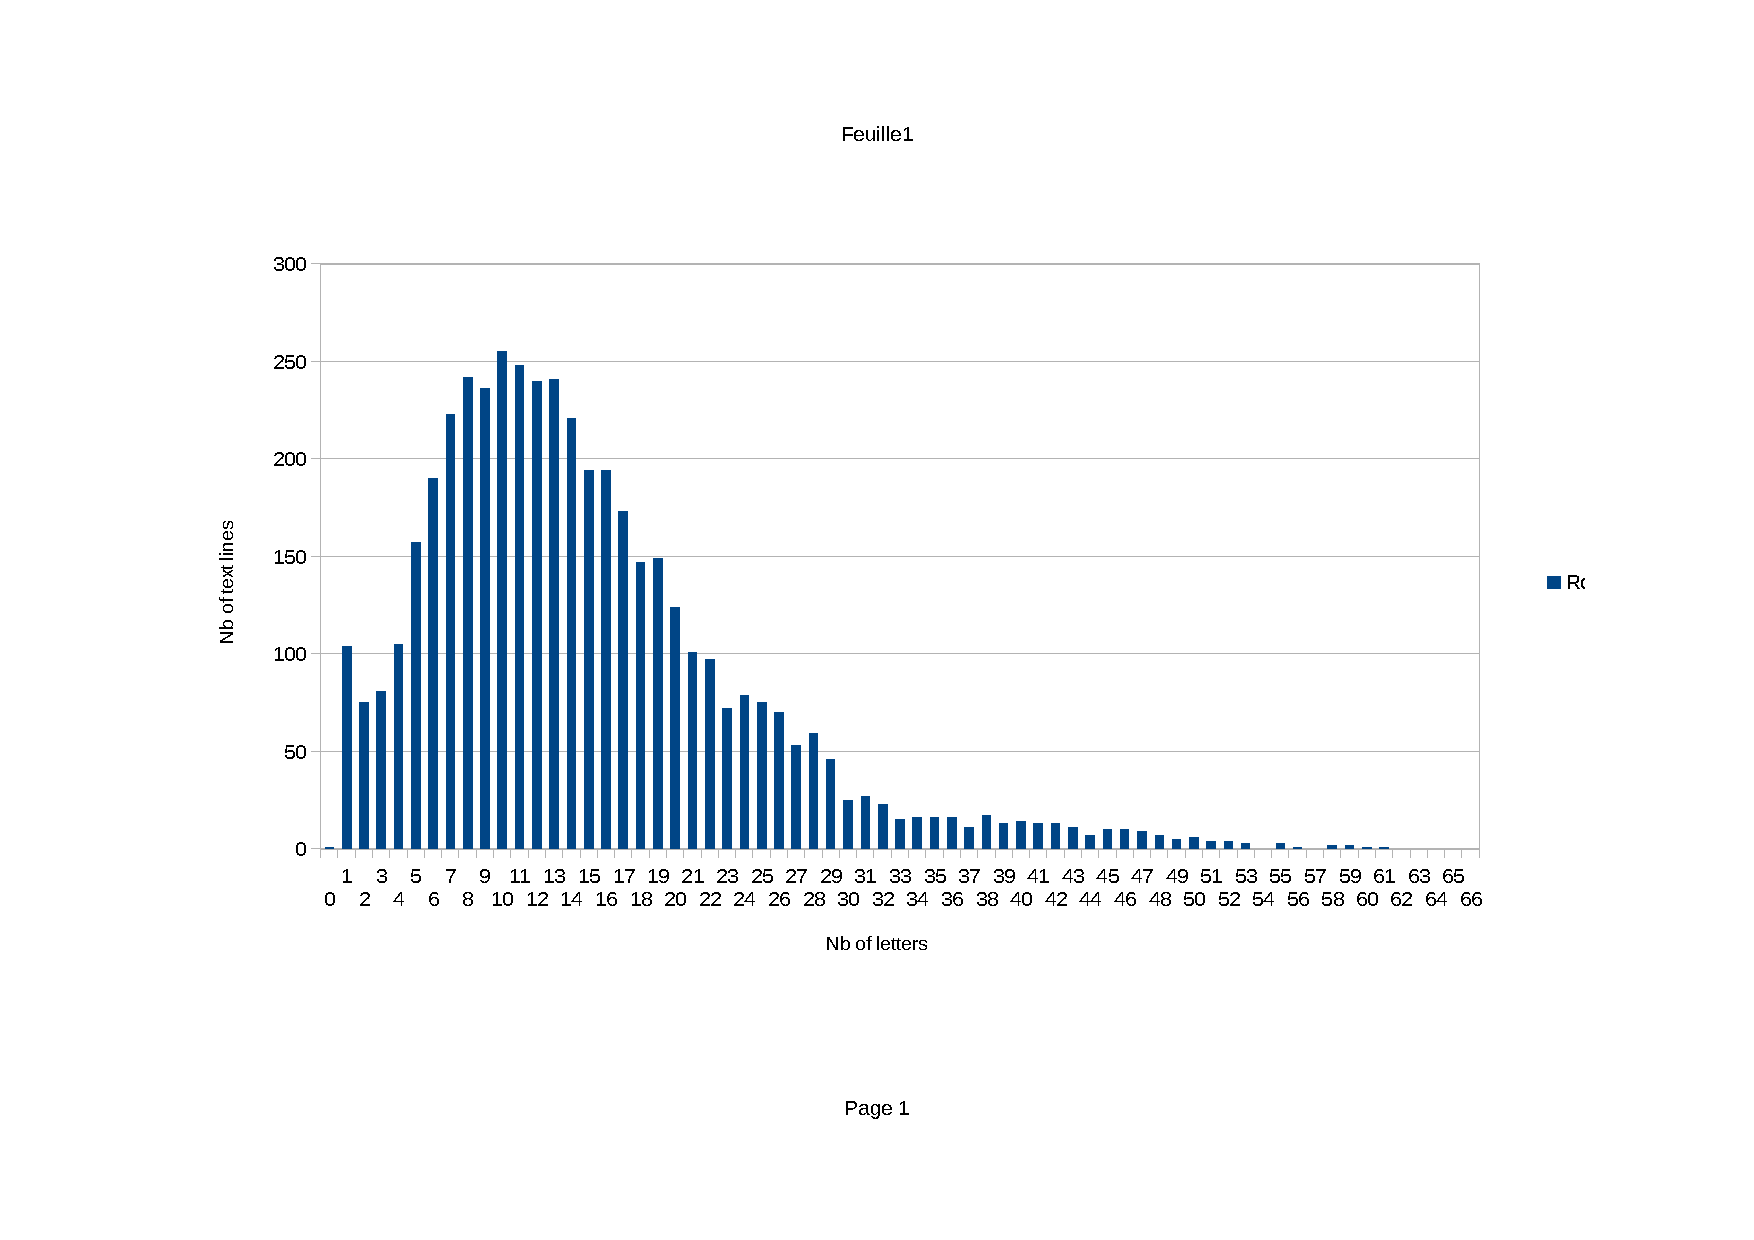
\includegraphics[trim= 100px 130px 120px 120px, clip, width=0.65\textwidth]{number_of_letter_per_textline.pdf}
      \caption{Distribution of the number of elements per text lines.
      }
      \label{fig:gt:textline_lenth_distribution}
    \end{figure}  
    %%%%%%%%%%%%%%%%%%%%%%%%%%%%%%%%%%%%%%%%%%%%%%%%%%%%%%%%

% paragraph text (end)

\paragraph{Comic characters} % (fold)
\label{par:comic_characters}
or protagonist are specific to each album.
They all have eye, harm and leg but at least 50\% are not humanoid, depending on the interpretation.
% paragraph comic_characters (end)

\subsection{Term of use} % (fold)
\label{sub:term_of_use}
We obtain the minimum rights for sharing and publishing image material from the right holders but we had to make sure the user accept it before using the data.
In collaboration with the intellectual property department of the University of La Rochelle, we established the following:

\textit{In order to use this database, you must firstly agree to the terms.
You may not use the database if you don't accept the terms.
The use of this database is limited to scientific and non-commercial purpose only, in the computer science domain.
For instance, you are allowed to split the images, through the use of segmentation algorithms.
You can also use pieces of this database to illustrate your research in publications and presentations.
Any other use case must be validated by our service.
If you do agree to be bound by all of these Terms of Use, please fill and email the request form and then use the login and password provided to download the selected version below.}

The concerned request form requires the identity, affiliation, address and intended use of the person who wishes to use data.

% subsection term_of_use (end)

\section{Ground truth construction} % (fold)
\label{sec:ground_truth_construction}
In order to cover a wide range of possible research matters, it has been decided to extract three different type of objects from the corpus: text lines, balloons and panels.
We decided to do this first ground truth by drawing horizontal bounding boxes as close as possible from the feature and including all its pixels.
% in order to proceed a maximum of pages in the allowed time. 
We chose this level of granularity in order to limit the subjectiveness of the person making the annotation.

The comics art is extremely heterogeneous and our dataset voluntarily integrates albums that can be classified as
unconventional.
This leaves room for interpretation on the form which increase annotation variations by different people and decrease the uniformity of the ground truth.
This precision level is used in several, widely used datasets~\cite{pascal-voc-2012, yao2007introduction}.
%{\color{blue}This groundtruthing level is also used for well known dataset widely used~\cite{pascal-voc-2012, yao2007introduction}.}

Hereafter we detail the two levels of annotation (visual and semantic) that form the ground truth and how they are indexed in a file.
The combination of visual and semantic annotation provides the advantage of making this ground truth relevant for document analysis and semantic evaluation which are both part of the comics understanding process.

% each element to annotate and the protocol to follow.
% follows specific guidelines according to the rules below:

\subsection{Visual annotation} % (fold)
\label{sub:visual_annotation}
The first annotation consist in defining the spacial region where elements are located in the image.
We describe hare how the visual annotation have been performed for the panels, balloons, texts and comic characters.

% subsection visual_annotation (end)
\paragraph{Panels} % (fold)
\label{par:panels}
The frame or panels are defined as an image area, generally rectangular, representing a single scene in the story. 
There is always at least one panel per page, the entire page region can be used as panel if necessary.
When a panel has a black border, the bounding box is placed as close as possible to its frame.
Sometimes, images have not been scanned perfectly horizontally, it is then impossible to have an horizontal bounding box sticking exactly to the border.
When the panel border is partially absent or suggested by the neighbourhood, the bounding box just defines the content of the panel.
In all cases, the other elements (balloon, text, drawings) extending from the frame are truncated, see figure~\ref{fig:gt:segPanel}.

%%%%%%%%%%%%%%%%%%%%%%%%%%%%%%%%%%%%%%%%%%%%%%%%%%%%%%%%%
\begin{figure}[h!]
\begin{center}
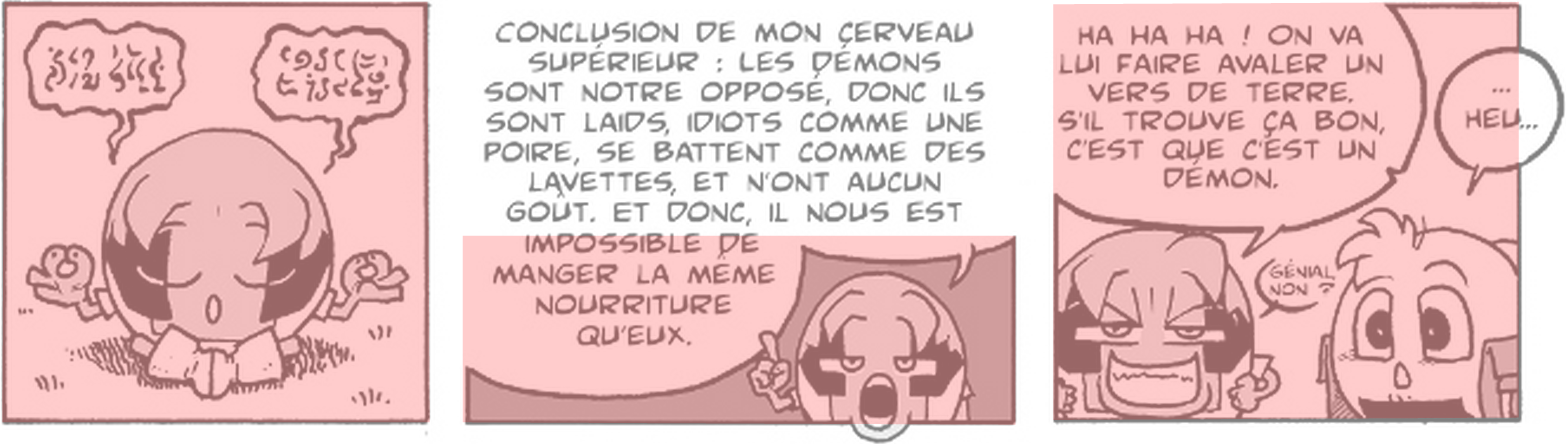
\includegraphics[width=0.8\textwidth]{segPanel.png}
\caption[Panel annotation]{Example of three panel annotations. The bounding box (transparent red) is defined without taking into account of non panel elements in all cases.}
\label{fig:gt:segPanel}
\end{center}
\end{figure}
%%%%%%%%%%%%%%%%%%%%%%%%%%%%%%%%%%%%%%%%%%%%%%%%%%%%%%%%%

%They can be frame-less, in that case the bounding box will be set according to the contained drawings, see Fig. \ref{fig:segmentation}c. %, ignoring text and overlapping features.
%In both cases, text and overlapping features are ignored.
%There is necessarily at least one panel in a page. 
% paragraph panels (end)

% The panel reading order is also annotated in a metadata called \texttt{rank}, it is in integer  between $1$ and $n$ which is increased incrementally from the first to the last panel $n$ in an image.%, le premier de la séquence prenant la valeur $1$ et le dernier la valeur $n$ pour une page contenant $n$ cases.

\paragraph{Balloons} % (fold)
\label{par:balloons}
We define a balloon (phylactery or bubble) as the region of an image including one or several lines of text, graphically defined by an identifiable physical boundary or suggested by the presence of an arrow pointing to the speaker (the tail).
Although rare, empty balloons (not containing lines of text) are also annotated if they are clearly identifiable by their shape or
the tail representation.
Pixel level annotation follows the contour of the balloon (see figure~\ref{fig:gt:segBalloons}c), while bounding box annotation does not consider the contour of phylactery and truncates the tail.
Sometimes it crosses the entire panel and generates an unrepresentative position of the desired balloon (see figure~\ref{fig:gt:segBalloons}a).
When the balloon is not closed (e.g. open contour) the annotated contour has to stick as close as possible to the contained text (see figure~\ref{fig:gt:segBalloons}b).
Note, the first version of the ground truth (2013) have been defined at bounding box level ignoring the tail and the second version (2014) at pixel level following the contour variations and the tail region.

%%%%%%%%%%%%%%%%%%%%%%%%%%%%%%%%%%%%%%%%%%%%%%ù
\begin{figure}[h!]
\begin{center}
\begin{tabular}{ccc}
a) 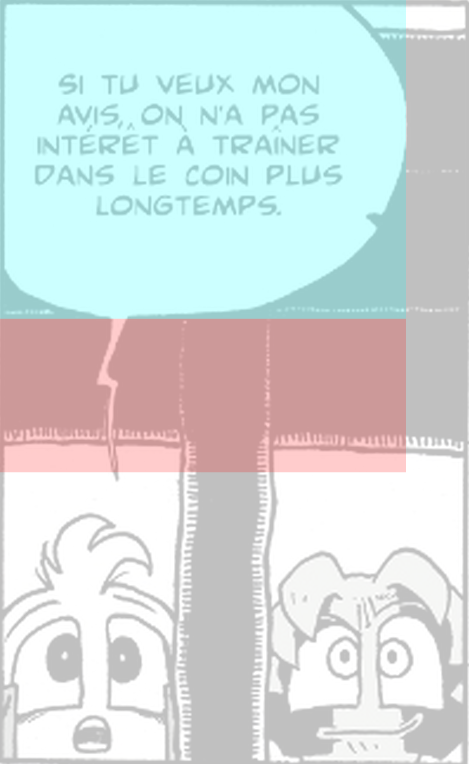
\includegraphics[width=80px]{segBalloon1.png} 
& 
b) 
\includegraphics[width=80px]{segBalloon2.png}
&
c) 
\includegraphics[width=80px]{segBalloon3.png}
\end{tabular}
\caption[Speech balloon contour annotation]{Example of balloon clipping: a) using bounding box excluding the tail, b) bounding box of non closed balloon, c) pixel level contour annotation.} 
\label{fig:gt:segBalloons}
\end{center}
\end{figure}
%%%%%%%%%%%%%%%%%%%%%%%%%%%%%%%%%%%%%%%%%%%%%%ù

% paragraph balloons (end)

\paragraph{Text lines} % (fold)
\label{par:text_lines}
The text lines are defined as a sequence of text characters aligned in the same direction (see figure~\ref{fig:gt:segLines}a).
This definition encompasses both speech texts and narrative text, often located inside balloon, onomatopoeia (graphic sound) that are written or drawn directly in the panel without particular container.
%The text of the latter, although they are occasionally parallel to the edges of the box is still clipped by a horizontal bounding box for consistency across the ground truth.
Comics are static graphics, the expression of emotions of a comic character is the joint action of drawing and text, sometimes in the form of a single punctuation symbol.
For instance, an exclamation mark for surprise or a question mark for a misunderstanding.
These isolated symbols convey information and are segmented as text line as well (see figure~\ref{fig:gt:segLines}b).
Similarly, we have chosen to include in this category the illustrative text, such as a road sign or storefront (see figure~\ref{fig:gt:segLines}c).
Although at the boundary between text and graphic, these elements are still invariably read by the reader and their annotation is potentially interesting for multiple purposes, including story and scene analysis.

%%%%%%%%%%%%%%%%%%%%%%%%%%%%%%%%%%%%%%%%%%%%%%ù
\begin{figure}[h!]
\begin{center}
\begin{tabular}{ccc}
a) 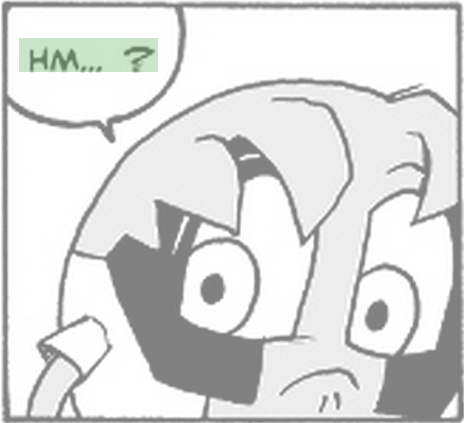
\includegraphics[width=80px]{segLine1.png} 
& 
b) 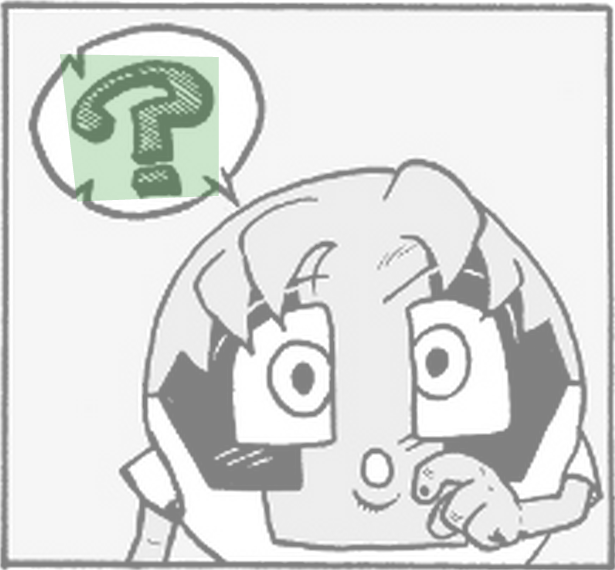
\includegraphics[width=80px]{segLine2.png}
&
c) 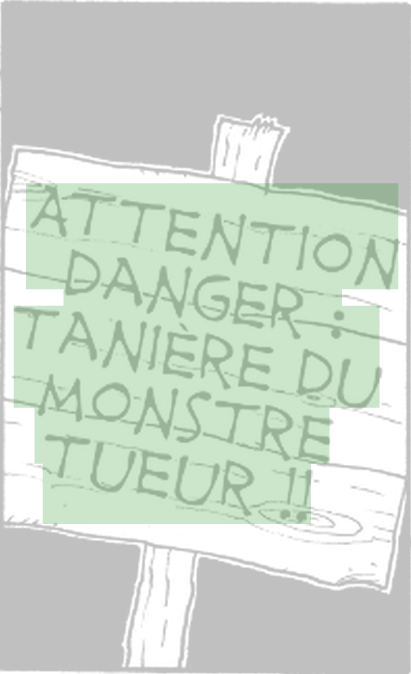
\includegraphics[width=80px]{segLine3.png}
\end{tabular}
\caption[Text line location annotation]{Different examples of text line position annotation: a) a classical text line in a speech balloon, b) a unique symbol, c) illustrative text, non horizontal.} 
\label{fig:segLines}
\end{center}
\end{figure}
%%%%%%%%%%%%%%%%%%%%%%%%%%%%%%%%%%%%%%%%%%%%%%ù

% paragraph text_lines (end)

\paragraph{Comic characters} % (fold)
\label{par:comic_characters}
The comic characters position have been included in the second version of the ground truth only (2014).
The concept of ``character'' may have different interpretations when used for comics and must be specified.
Characters in a comic have not necessarily a human-like, or even living beings appearance.
Even so, it would be appropriate to annotate every human being appearing in a box while some are nothing but a part of the scenery.
Therefore, we have chosen to limit the annotation to the comic characters that emits at least one speech balloon in the album (minimal impact in the story).
Their bounding box has been defined to maximize the region occupied by the comic character inside the box region.
Therefore, some parts of the character such as arms or legs, are clipped sometimes (see figure~\ref{fig:gt:segCharater}).

%%%%%%%%%%%%%%%%%%%%%%%%%%%%%%%%%%%%%%%%%%%%%%
\begin{figure}[h!]
\begin{center}
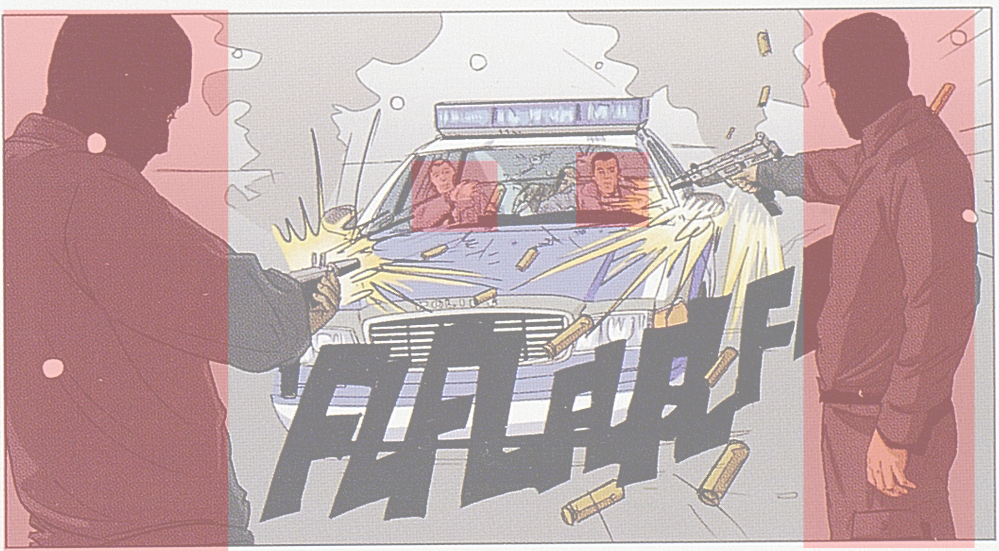
\includegraphics[width=0.75\textwidth]{segCharacter.png}
\caption[Comic character position annotation]{Example of comic character annotation: sniper's arms are not included in the bounding box in order to maximize the region occupied by the sniper in its bounding box. The two snipers and the two characters in the car are annotated because they emit a speech balloon in a different panel.}
\label{fig:gt:segCharacter}
\end{center}
\end{figure}
%%%%%%%%%%%%%%%%%%%%%%%%%%%%%%%%%%%%%%%%%%%%%%

% paragraph comic_characters (end)


% section ground_truth_construction (end)

\subsection{Semantic annotation} % (fold)
\label{sub:gt:semantic_annotation}
This second level of annotation complete each spacial region with additional information about its semantic.
Also, the image itself is annotated with extra information about its origin (e.g. album, collection, author, publisher).
%Once segmented, each object is annotated with a set of predefined metadata as follows. 

\paragraph{Images}
The image, often assimilated as pages, has been annotated with bibliographical information, so that anyone using this ground truth is free to get is own paper copy of the comic books for extra uses.
The first annotation is the page number (\texttt{{pageNumber}}) then the comic book title, from which the page has been picked up, and its release date (\texttt{{albumTitle, releaseDate}}), the series it belongs to (\texttt{{collectionTitle}}), the authors and editor names (\texttt{{writerName, drawerName, editorName}}) and, finally, the website and/or ISBN (\texttt{{website, ISBN}}).
The album title is not mandatory for webcomics.
Structural information about the page content has been added as well, such as resolution (\texttt{{resolution}}), reading direction (\texttt{{readingDirection}}), main language of the text (\texttt{{language}}) and single or double page information (\texttt{{doublePage}}).
% These annotation are stored in a tag named \texttt{{Pages}}.

\paragraph{Panels} 
The panes are annotated with a \texttt{{rank}} metadata which stand for its position in the reading sequence. 
The first panel to be read on a given page has its rank property set to 1, while the last one is set to \textit{n}, where \textit{n} is the number of panels in the page.

\paragraph{Balloons}
Balloons are also annotated with a \texttt{{rank}} property that defines their reading order relatively to the image because balloons are not always included in panels.
%, their rank is set according to the page as a whole. 
For a page containing $m$ balloons, the first balloon's rank will be 1 and the last will be $m$.
%Moreover, two additional metadata are given. 
A second information concerns the \texttt{{shape}} of the balloon.
This feature conveys an information about how the contained text is spoken (tone).
The type of \texttt{{shape}} is given from the following list \{\texttt{smooth, wavy, spiky, suggested}\} as pictured in figure~\ref{fig:gt:balloonShape}.
Finally, the tail tip position (extremity) and its pointing direction have been added into the second version of the ground truth.
There are given through the \texttt{{tailTip}} and \texttt{{tailDirection}} properties.
The possible values of the direction are reduced to the eight cardinal directions plus a ninth additional value for the lack of tail: \{\texttt{N, NE, E, SE, S, SW, W, NW, none}\}.
In the second version of the ground truth (2014), we added the identifier of the comic character which is emitting the balloon \texttt{{idCharacter}}. 

%%%%%%%%%%%%%%%%%%%%%%%%%%%%%%%%%%%%%%%%%%%%%%%%%%%
\begin{figure}[h!]
\begin{center}
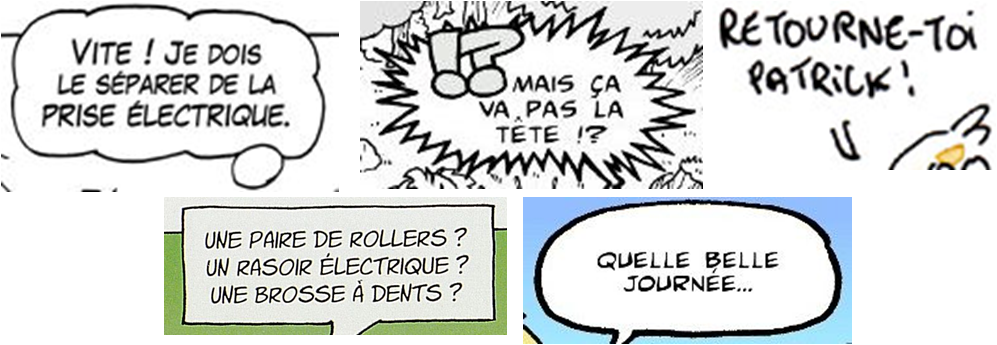
\includegraphics[width=0.65\textwidth]{balloonShape.png}
\caption[Balloon shapes]{Les différents types de contour de bulle, de gauche à droite et de haut en bas : nuage, hérissé, suggéré, rectangle, ovale.}
\label{fig:gt:balloonShape}
\end{center}
\end{figure}
%%%%%%%%%%%%%%%%%%%%%%%%%%%%%%%%%%%%%%%%%%%%%%%%%%%

\paragraph{Text lines}
The text lines are associated with their transcription and the identifier of the corresponding balloon is added in \texttt{{idBalloon}} if the text line is included in a balloon.

\paragraph{Comic characters} % (fold)
\label{par:comic_characters}
The comic character are identified by \texttt{{idCharacter}} in order to be easily referred.

% paragraph comic_characters (end)

% \paragraph{Speaking character and speech balloon} % (fold)
% \label{par:speaking_character_and_speech_balloon}
% In the second version of the ground truth, we added a new type of relation which is between regions.
%  balloons and comic characters regions that are related in the story (balloon spoken by a character).
% The information is stored in a structure called \texttt{{LinkSBSC}} that consist a pair of identifier \texttt{{idBalloon}} and \texttt{{idCharacter}}.
% paragraph speaking_character_and_speech_balloon (end)


%%%%%%%%%%%%%%%%%%%%%%%%%%%%%%%%%%%%%%%%%%%
% \begin{figure}
% \begin{center}
% \includegraphics[width=0.45\textwidth]{balloons_shape3.png}
% \caption{Different speech balloon shapes. Top-down, from left to right: cloud, peak, suggested, rectangular and oval.}
% \label{fig:balloons_shape}
% \end{center}
% \end{figure}
%%%%%%%%%%%%%%%%%%%%%%%%%%%%%%%%%%%%%%%%%%%

% subsection semantic_annotation (end)

\subsection{File structure} % (fold)
\label{sub:file_structure}

The ground truth file structure have been thought according to comics related formalism such as Comics Markup Language (ComicsML)~\cite{McIntosh2011}, Comic Book Markup Language (CBML)~\cite{Walsh2012a}, Periodical Comics\footnote{\url{http://www.w3.org/wiki/WebSchemas/PeriodicalsComics}}, A Comics Ontology~\cite{Rissen2012}, Advanced Comic Book Format (ACBF)\footnote{\url{https://launchpad.net/acbf}} and the Grand Comics Database (GCD)\footnote{\url{http://www.comics.org}}.
See the Ph.D. thesis of Gu{\'e}rin~\cite{phdthesisGuerin14} for an extended review.

As we wanted to keep the ground truth file system simple and easy to share, visual and semantic annotations about a given page are gathered in a single full-text file following the specifications of Scalable Vector Graphics (SVG). 
Besides being an open-standard developed by the World Wide Web Consortium (W3C) since 1999, the SVG format fulfils two essential needs for this database.

First, using a recent Internet browser or your favourite image viewer, it provides a simple, fast and elegant way to display the visual annotation of any desired object over a comic book page using layers.
No need to install software such as Matlab, Adobe Illustrator or equivalent open source to visualize the ground truth information.

It is XML-based vector image format that allows to display an animate the annotated region, stored as polygon object in the SVG file, as desired using the Cascading Style Sheets (CSS) properties, see figure~\ref{fig:gt:svgImage}. 

%%%%%%%%%%%%%%%%%%%%%%%%%%%%%%%%%%%%%%%%%%%%%%%%%

\begin{figure}[h!]
\begin{center}
\begin{tabular}{ccc}
a) 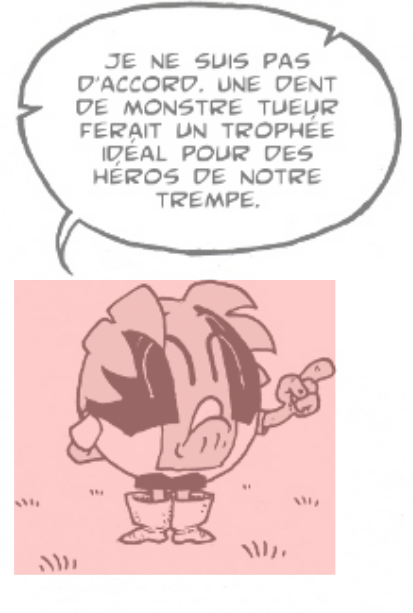
\includegraphics[width=100px]{svgPanel.png} 
& 
b) 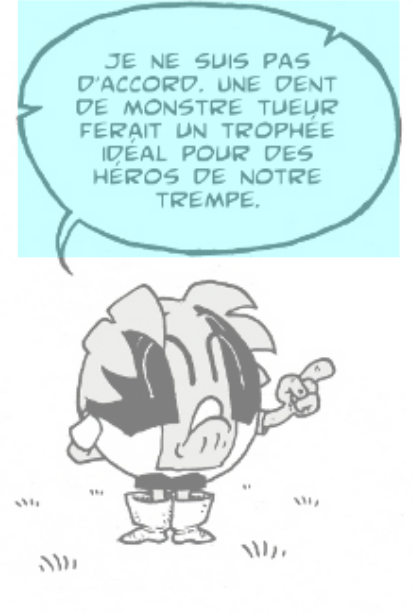
\includegraphics[width=100px]{svgBalloon.png}
&
c) 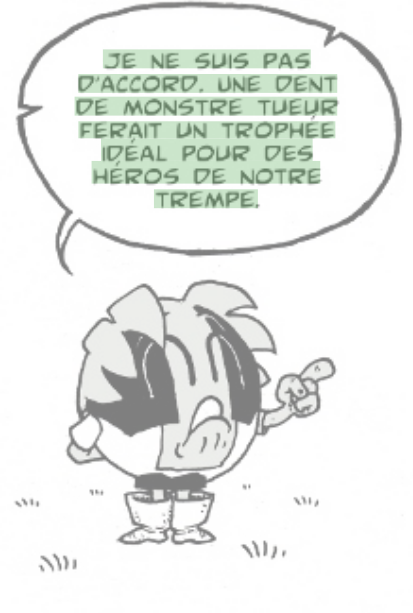
\includegraphics[width=100px]{svgTextlines.png}
\end{tabular}
\caption[Annotation rendering in a browser]{Example of rendering for each class of element. For example, red for panels (a), cyan for balloons (b) and green for text (c). The opacity is set to 50\% to allow seeing the corresponding image by transparency.} 
\label{fig:gt:svgImage}
\end{center}
\end{figure}
%%%%%%%%%%%%%%%%%%%%%%%%%%%%%%%%%%%%%%%%%%%%%%%%%%

Each layer can be displayed or not in order to enhance the clearness of the annotations when browsing the database.
Secondly, SVG being a XLM-based language, it makes the integration of semantic annotation very easy via the use of the predefined \texttt{metadata} element.

One ground truth file contains the complete description of one comics image. 
There is no hierarchical link between pages from a same comic book. 
Following the basic XML encoding information, a SVG file starts with a root \texttt{<svg>} element containing the title of the document, \texttt{<title>}, and five \texttt{<svg>} children with different class attributes.
These contain annotations collected on five types of elements which are the page, panels, balloons, text lines and comic characters.
The type of element in a tag is specified by its \texttt{class} attribute.
The first tag, \texttt{class = ``Page''} contains description on the image and has two daughters.
The first one, \texttt{image} has several attributes which specifies a link to the image file in the dataset \texttt{xlink: href} and two specifying the \texttt{width} and \texttt{height} of the image.
The second, \texttt{metadata}, contains bibliographic information about the album and page properties described in \ref{sub:gt:semantic_annotation}.
%A SVG file begins with information about the XML version and encoding system and then a root \texttt{<svg>} element containing the title of the document \texttt{<title>} and four others \texttt{<svg>} elements with different class attributes. % that describe the page, the panels, the text lines and the text areas the entire set of annotations for the attached page.
%The annotations are the same for all the \texttt{<svg>} nodes, each of them describing one kind of element (e.g. panel, balloon) according to its {\tt class} attribute. 
%The first \texttt{<svg>} element, \texttt{<svg class=``Page''>}, has two children.
%The first one is \texttt{<image>} and contains a link to the corresponding image file and the size it has to be displayed.
%The next child is a \texttt{<metadata>} element containing the bibliographical information described in \ref{sub:gt:semantic_annotation}.
The four following \texttt{<svg>} siblings, \texttt{<svg class=``Panel''>}, \texttt{<svg class=``Balloon''>}, \texttt{<svg class=``Line''>} and \texttt{<svg class=``Character''>} respectively contain the annotations about panels, balloons, text lines and comic characters. 
They all contain SVG \texttt{<polygon>} elements with a list of five or more points in a \texttt{point} attribute that define the position of the bounding box corners or the pixel-level contour. %four corners position coordinates of a bounding box. 
Note that the last point is always equal the first one to ``close'' the polygon according to the SVG specifications. 
Those points are used by the viewer to draw polygons with the corresponding CSS style. 
Each \texttt{<polygon>} has a \texttt{<metadata>} child to store information on the corresponding polygon, according to the attributes list described in \ref{sub:gt:semantic_annotation}.

An example of ground truth file is given figure~\ref{list:svg}.% présente un exemple du contenu de l'un de ces fichiers.

\begin{lstlisting}[language=XML, frame=single, caption=Example of SVG file of the eBDtheque ground truth, captionpos=b, label=list:svg]
<?xml version="1.0" encoding="UTF-8" standalone="no"?>
<svg>
  <title>CYB_BUBBLEGOM_T01_005</title>
  <svg class="Page">
    <image 
    	x="0" 
    	y="0" 
    	width="750" 
    	height="1060" 
    	href="CYB_BUBBLEGOM_T01_005.jpg"
    />
    <metadata 
    	collectionTitle="Bubblegom_Gom"
    	editorName="Studio_Cyborga" 
    	doublePage="false"
    	website="http://bubblegom.over-blog.com"
    	albumTitle="La_Legende_des_Yaouanks"
    	drawerName="Cyborg_07"
    	language="french"
    	resolution="300"
    	ISBN="979-10-90655-01-0"
    	readingDirection="leftToRight" 
    	writerName="Cyborg_07"
    	releaseDate="2009"
    	pageNumber="5"
    />
  </svg>
  <svg class="Panel">
    <polygon points="53,95 268,95 268,292 53,292 53,95">
      <metadata rank="1"/>
    </polygon>
    ...
  </svg>
  <svg class="Balloon">
    <polygon points="61,103 143,103 143,172 61,172 61,103">
      <metadata
      	idBalloon="B01" 
      	idCharacter="C01" 
      	shape="smooth"
      	tailDirection="SE" 
      	rank="1"
      />
    </polygon>
    ...
  </svg>
  <svg class="Line">
    <polygon points="373,121 432,121 432,132 373,132 373,121">
      <metadata idBalloon="B01">
      	LIKE YOU.
      </metadata>
    </polygon>
    ...
  </svg>
  <svg class="Character">
    <polygon points="84,153 261,153 261,298 84,298 84,153"/>
    	<metadata idCharacter="C01"/>
    ...
  </svg>
</svg>
\end{lstlisting}

%{\bf Add SVG code figure here?} Arnaud suggested it too but, we don't have room and it will be ugly...

%
%\begin{lstlisting}
%<svg>
%</svg>
%\end{lstlisting}

%{\color{red}short file as an illustration?}

% \begin{figure}
% \begin{center}
% \begin{tabular}{ccc}
% \includegraphics[width=0.14\textwidth]{fig/bbg_panel2.png} & 
% \includegraphics[width=0.14\textwidth]{fig/bbg_balloon2.png} &
% \includegraphics[width=0.14\textwidth]{fig/bbg_textlines2.png}
% %\includegraphics[width=0.20\textwidth]{fig/bbg_all.png} &
% \end{tabular}
% \caption{Left-to-right: segmentation of a panel, a speech balloon and text lines. Credits: \cite{Bubble09}}
% \label{fig:css}
% \end{center}
% \end{figure}
% subsection file_structure (end)

\begin{itemize}
	\item Comic Book Markup Language \url{http://digitalhumanities.org/dhq/vol/6/1/000117/000117.html}
\end{itemize}

\section{Ground truth quality assessment}
\label{sec:gt:ground_truth_quality_assessment}

When several persons are involved in the creation of a graphical ground truth, it is very difficult to obtain a perfectly homogeneous segmentation.
Indeed, it could vary from one person to another because each person has a different sensitivity at reading comics and at integrating instructions.
Therefore, in addition to the package of pages he was in charge of, each participant has been asked to annotate the panels of a extra page. 
This extra page was the same for everybody and was chosen for its graphical components heterogeneity. 
It contained ten panels from which, four were full-framed, five half-framed and one was frame less.
%, see Fig. \ref{fig:test_page}. 
% This heterogeneity is somehow representative of the whole corpus.
We defined an acceptable error for the position of a corner given by several persons.
The images of dataset being of different definitions, using a percentage of the page size makes more sense than using a specific number of pixels.
%A percentage of the page width and height is more relevant.
%Let set an acceptable error of 0.5\% of the page for the position on each corner. 
We set this percentage $p$ at 0.5\% of the page height and width in $x$ and $y$. 
Given the definition of the test image of 750x1060 pixels, this makes a delta of +/- 5 pixels in $y$ axis and +/- 4 pixels in $x$ axis. 

We asked to each one of the twenty involved persons to draw the four points bounding box of the panels ignoring text area.
A mean position from the twenty different values has been calculated for each of them.
Then, the distance of each point to its mean value is computed. 
Figure~\ref{fig:gt:graphiqueStdVT} shows the amount of corners for a distance, centred on zero.


%%%%%%%%%%%%%%%%%%%%%%%%%%%%%%%%%%%%%%%%%%%%%ù
\begin{figure}[h!]
\begin{center}
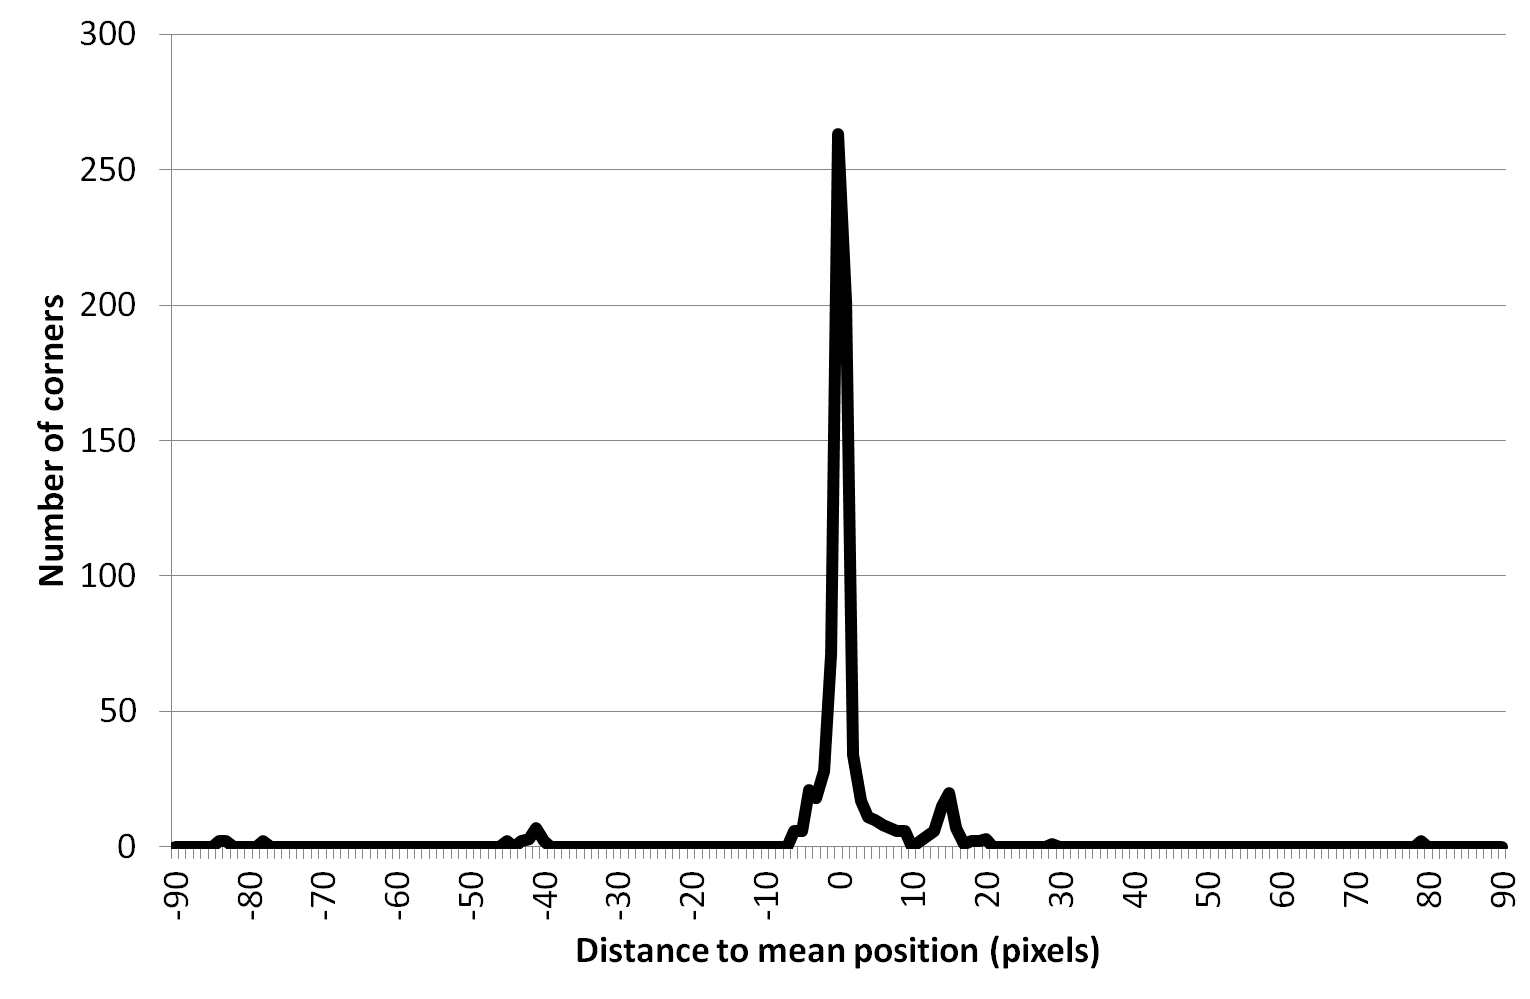
\includegraphics[width=0.7\textwidth]{stdVT.png}
\caption[Distance to the mean position]{Number of corners for a given standard deviation value. This has been calculated on $y$ axis and $x$ axis and produces similar plot.}
\label{fig:gt:graphiqueStdVT}
\end{center}
\end{figure}
%%%%%%%%%%%%%%%%%%%%%%%%%%%%%%%%%%%%%%%%%%%%%ù

Given the threshold $p=0.5$, 87.5\% of pointed corners can be considered as being homogeneous over the group of labelling people. 
%{\bf what is p?} p is the threshold
The overall mean standard deviation on this page reaches 0,15\%
 (1.13 pixels) for the width, and 0.12\% (1.28 pixels) for the height.
The two bumps, at -40 and 15, are related to the missegmentation of 13 of the 80 panels. 
Indeed, instructions have been misunderstood by some people who included text area outside of the panels or missed some panel's parts.
Figure~\ref{fig:gt:diffVT} shows the difference between areas labelled as a panel by at least one person and areas labelled as a panel by every participant.
However, such mistakes have been manually corrected before publishing the ground truth.

%%%%%%%%%%%%%%%%%%%%%%%%%%%%%%%%%%%%%%%%%%%%%%%%%
\begin{figure}[h!]
\begin{center}
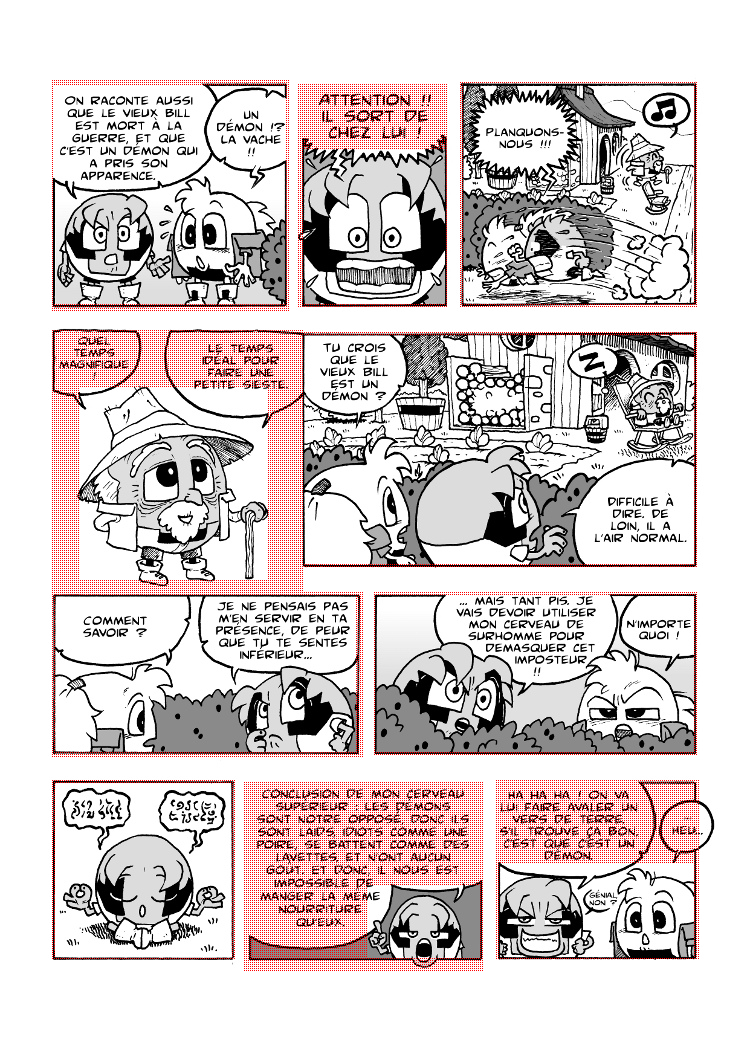
\includegraphics[width=0.7\textwidth]{segDifference.png}
\caption[Error measurement image]{Error measurement page. Red hatched areas are the difference between areas labelled as panels by at least one person, and areas labelled by everybody. Image credit:~\cite{Bubble09}.}
\label{fig:gt:diffVT}
\end{center}
\end{figure}
%%%%%%%%%%%%%%%%%%%%%%%%%%%%%%%%%%%%%%%%%%%%%%%%%

Even though the error criterion has only been estimated on panels, it is reasonable to extend it to balloons and text lines as well.
Indeed, the segmentation protocol being quite similar for all features (bounding box as close as possible to the drawing), the observed standard deviation of panel corner positions has no reason to be different from balloons and text lines.
The pixel-level balloon and the comic characters visual annotation have been carried out by a single person, the homogeneity is only subject to the regularity of the person over time and is, therefore, difficult to assess quantitatively.

% \section{Discussions}
% \label{sec:gt:siscussions}


\section{Conclusions}
\label{sec:gt:concl}
We presented the eBDtheque, a representative database of comics, which is composed by comics images, visual (spatial) and semantic annotations.
The one hundred image corpus has been introduced as well as its ground truth construction and quality assessment protocols.

The material have been published in 2013~\cite{Guerin2013} and made available to the scientific community via the project website~\footnote{http://ebdtheque.univ-lr.fr}.

\modif{At the time this thesis is written, five requests from India, China and Japan have been received to use this dataset and ground truth.}

% In order to provide a common basis for evaluating research work, the ground truth have been published
% It has been enhanced in 2014 by adding semantic information to the already annotated elements.


\chapter{Panel extraction}
\chaptermark{Panel extraction}
\label{chap:intro}
\graphicspath{{./chapters/4-pe/figs/}}

% Introduction
\section{Introduction}
\label{sec:pe:introduction}

% Contributions -------------------------------------------------------------------------------------------------------------------------------------------
\section{Methodology (contribution)}
\label{sec:pe:methodology}

% Experiments --------------------------------------------------------------------------------------------------------
\section{Experimental results}
\label{sec:pe:experimental_results}


% Conclusion --------------------------------------------------------------------------------------------------------------------------------------
\section{Conclusions}
\label{sec:pe:conclusion}

\chapter{Balloon segmentation and classification}
\chaptermark{Balloon segmentation and classification}
\label{chap:balloon_segmentation_and_classification}
\graphicspath{{./chapters/6-be/figs/}}

% Introduction
\section{Introduction}
\label{sec:be:introduction}


% Contributions -------------------------------------------------------------------------------------------------------------------------------------------
\section{Methodology}
\label{sec:be:methodology}

\subsection{Localization} % (fold)
\label{sub:be:localization}

% subsection localization (end)

\subsection{Segmentation \& classification} % (fold)
\label{sub:be:segmentation}
\begin{itemize}
	\item Balloon type study: The Rise and Reason of Comics and Graphic Literature: Critical Essays on the Form chapter 4 \url{http://afflatus.ucd.ie/Papers/comics%202010.pdf} or \url{/Biblio_LINK/Bandes_dessinées/2010_Forceville_Balloonics: The Visuals of Balloons in Comics.pdf} and \url{http://books.google.fr/books?id=8yXWG0efa_8C&printsec=frontcover&source=gbs_ge_summary_r&cad=0#v=onepage&q&f=false}
	\item Publication GREC'13 + LNCS'14 (not published yet) \url{/home/crigau02/Bureau/PhD/research/balloon_classification/output/publication/GREC/paper}
\end{itemize}

% subsection segmentation (end)

\subsection{Tail detection and description} % (fold)
\label{sub:be:tail_detection_and_description}

% subsection tail_detection_and_description (end)

% Experiments --------------------------------------------------------------------------------------------------------
\section{Experimental results}
\label{sec:be:experimental_results}


% Conclusion --------------------------------------------------------------------------------------------------------------------------------------
\section{Conclusions}
\label{sec:be:conclusion}

\chapter{Text localization and recognition}
\chaptermark{Text localization and recognition}
\label{chap:text_localization}
\graphicspath{{./chapters/5-te/figs/}}

% Introduction
\section{Introduction}


% Contributions -------------------------------------------------------------------------------------------------------------------------------------------
\section{Methodology}

\subsection{Text localization} % (fold)
\label{sub:text_localization}

% subsection text_localization (end)

\subsection{Text recognition} % (fold)
\label{sub:text_recognition}

% subsection text_recognition (end)

% Experiments --------------------------------------------------------------------------------------------------------
\section{Experimental results}


% Conclusion --------------------------------------------------------------------------------------------------------------------------------------
\section{Conclusions}

\chapter{Comic character spotting and clustering}
\chaptermark{Comic character spotting}
\label{chap:ce}
\graphicspath{{./chapters/1-introduction/figs/}}

% Introduction
\section{Introduction}
\label{sec:ce:introduction}

% Contributions -------------------------------------------------------------------------------------------------------------------------------------------
\section{Methodology}
\label{sec:ce:methodology}

\subsection{Detection and spotting} % (fold)
\label{sub:ce:detection_and_spotting}

\begin{itemize}
	\item Insist on the key point of DAS'14 publication: the colour selection method for the object descriptor.
\end{itemize}
% subsection detection_and_spotting (end)

\subsection{Clustering} % (fold)
\label{sub:ce:clustering}

% subsection clustering (end)


% Experiments --------------------------------------------------------------------------------------------------------
\section{Experimental results}
\label{sec:ce:experiments}

% Conclusion --------------------------------------------------------------------------------------------------------------------------------------
\section{Conclusions}
\label{sec:ce:conclusion}

%\chapter{Comics image processing}
\chaptermark{Comics image processing}
\label{chap:lp}
\graphicspath{{./chapters/4-lp/figs/}}

%Abstract-------------------------------------------------------------------------------------------------------------
%In this chapter we propose a symbol spotting technique in graphical documents. Graphs are used to represent the documents and an error tolerant (sub)graph matching technique is used to detect the symbols in them. We propose a graph serialization to reduce the usual computational complexity of graph matching. Serialization of graphs is performed by computing acyclic graph paths between each pair of connected nodes. Graph paths are one dimensional structures of graphs, handling which is less expensive in terms of computation. At the same time they enable robust localization even in the presence of noise and distortion. Indexing in large graph databases involves a computational burden as well. We utilize a graph factorization approach to tackle this problem. Factorization is intended to create a unified indexed structure over the database of graphical documents. Once graph paths are extracted, the entire database of graphical documents is indexed in hash tables by locality sensitive hashing (LSH) of shape descriptors of the paths. The hashing data structure aims to execute an approximate $k$-NN search in a sub-linear time. We have performed detailed experiments with various datasets of line drawings and the results demonstrate the effectiveness and efficiency of our technique.
%----------------------------------------------------------------------------------------------------------------------
\section{Introduction}
\label{sec:hssg:intro}



\section{Panel extraction}
\label{sec:hssg:meth}


\section{Balloon segmentation}
\label{ssec:hssg:frwrk}


% \subsection{Closed balloons}
% \label{ssec:lp:balloon_closed}


% \subsection{Open balloons}
% \label{ssec:lp:balloon_open}


\section{Text extraction}
\label{ssec:hssg:pthdesc}



\section{Character spotting and identification}
\label{ssec:hssg:vot}


\section{Conclusions}
\label{sec:hssg:concl}

%In this chapter we have proposed a graph based approach for symbol spotting in graphical documents. We represent the documents with graphs where the critical points detected in the vectorized graphical documents are considered as the nodes and the lines joining them are considered as the edges. The document database is represented by the unification of the serialized substructures of graphs. Here the graph substructures are the acyclic graph paths between each pair of connected nodes. The factorized substructures are the one-dimensional (sub)graphs which give efficiency in terms of computation and since they provide a unified representation over the database, the computation is substantially reduced. Moreover, the paths give adaptation to some structural errors in documents with a certain degree of tolerance. We organize the graph paths in hash tables using the LSH technique, this helps to retrieve symbols in real time. We have tested the method on different datasets of various kinds of document images and the results are quite encouraging.

%In the next chapter we are going to propose a subgraph matching algorithm based on tensor product graph (TPG) (see \sect{sec:gm:pg} for details). Continuous optimization is a very popular approach in (sub)graph matching but it mostly works with pairwise measurements. But often pairwise quantifications are not reliable, to remove this problem in \ch{chap:pg} we propose walk based propagation of pairwise similarities to obtain contextual information incorporated in the higher order similarity measures. Then we formulate the subgraph matching problem as a node, edge selection problem in TPG. Also in \ch{chap:pg}, a \emph{dual edge graph} representation is proposed which achieves spatial relationship between the graph paths which was absent in this chapter.
\chapter{System for document understanding} % 20 pages (see Clement's work)
\chaptermark{System for document understanding}
\label{chap:hp}
\graphicspath{{./chapters/8-hp/figs/}}

% Abstract------------------------------------------------------------------
In literature, there are methods that formulate...

\section{Introduction}
\label{sec:hp:intro}


%------------------------------------------------------------------------------------------------------------------------------------------------------------------------------------------------------------
\section{Methodology}
\label{sec:hp:method}


\subsection{Framework}
\label{sub:hp:rw}


\subsection{Application to comics} % (fold)
\label{sub:hp:application_to_comics}


\begin{equation}
SW_X=\lim_{n\rightarrow \infty}\sum_{k=0}^n \lambda^k W_{X_k}
\label{eqn:pg:rw1}
\end{equation}

where
\begin{equation}
W_{X_k} = W_X^k
\end{equation}

Here $\lambda$ is a weighting factor to discount the longer walks, as they often contain redundant or repeated information. In this chapter we always choose $\lambda=\frac{1}{a}$, where $a=\min(\Delta^+(W_X),\Delta^-(W_X))$. Here $\Delta^+(W_X)$, $\Delta^-(W_X)$ are respectively the maximum outward and inward degree of $W_X$~\cite{Gartner2003a}.

\section{Experimental results} % (fold)
\label{sec:hp:experimental_results}

% section experimental_results (end)

%------------------------------------------------------------------------------------------------------------------------------------------------------------------------------------------------------------
\section{Conclusions}
\label{sec:hp:conclusion}

%\input{./chapters/7-hgr/hgr}
%\chapter{Experimental Evaluation}
\chaptermark{Experiments}
\label{chap:experiments}
\graphicspath{{./chapters/8-experiments/figs/}}
The main purpose of this chapter is to provide an overall experimental evaluation and comparison of all the proposed methodologies and some of the state-of-the-art methods proposed in the literature. Among the state-of-the-art methods we have considered those which work with graph based techniques and apply their algorithms for symbol spotting in graphical documents. To have a unified experimental framework we configure a symbol spotting system on graphical documents especially on architectural floorplans. The evaluation of a particular method is basically done depending on the capability of spotting symbols on the graphical document.
\section{Introduction}
\label{sec:experiments:intro}
In the previous four chapters we have provided individual experiments corresponding to the different contributions of the thesis. In this chapter we provide an integrated evaluation scheme. Experimental evaluation is an important step to judge the behaviour of algorithms. An experimental study should reveal the strengths and weaknesses of the methods under test. The analysis of these strong points and drawbacks should determine which method is the most suitable for a certain use case and predict its behaviour when using it in applications with real data. In this chapter, we experimentally evaluate the proposed and some of the state-of-the-art algorithms and provide an overall comparisons among them.

Before going to the results part, in the next section we have provided a brief description of the state-of-the-art algorithms on symbol spotting considered for the comparison. For referencing the algorithms we use some abbreviations of the names which are listed in Table~\ref{tab:experiments:references}.

\begin{table}[h!]
\centering
\caption{Summary, abbreviations of the methods}
\begin{tabular}{r|m{9.5cm}}
\toprule
\hline
\textbf{Abbreviation} & \textbf{Method}\\
\hline
SG & Symbol spotting by hashing of serialized subgraphs (\ch{chap:hssg}).\\
PG & Product graph based subgraph matching (\ch{chap:pg}).\\
NCRAG & Near convex region adjacency graph (\ch{chap:ncrag}).\\
HGR & Hierarchical graph representation (\ch{chap:hgr}).\\
SSGR & Symbol spotting using graph representations~\cite{Qureshi2007}\\
FGE & Subgraph spotting through fuzzy graph embedding~\cite{Luqman2011}.\\
ILPIso & Integer linear program for substitution tolerant subgraph isomorphism~\cite{LeBodic2012}.\\
\hline
\end{tabular}
\label{tab:experiments:references}
\end{table}

The rest of the chapter is divided into four sections, where \sect{sec:experiments:desc-sota} is dedicated for describing in brief the state-of-the-art methods that we have considered for experimental evaluation and comparison. The experimentation is described in \sect{sec:experiments:res}. \sect{sec:experiments:disc} contains discussions on the obtained results by various methods. After that in \sect{sec:experiments:concl} the chapter is concluded.

\section{Description of state-of-the-art methods}
\label{sec:experiments:desc-sota}
This section contains brief descriptions of the three state-of-the-art methods:

\textbf{Symbol spotting using graph representations~\cite{Qureshi2007}:} The algorithm was proposed by Qureshi~\etal~\cite{Qureshi2007}. The proposed strategy has two main steps. In the first step, a graph based representation of a document image is generated that includes selection of description primitives (nodes of the graph) and relation of these features (edges) (see \fig{fig:experiments:ssgr}). In the second step the graph is used to spot interesting parts of the image that potentially correspond to symbols. The sub-graphs associated to selected zones are then submitted to a graph matching algorithm in order to take the final decision and to recognize the class of the symbol. The experimental results obtained on different types of documents demonstrates that the system can handle different types of images without any modification.
\begin{figure}[t!]
\begin{center}
\subfloat[]{\includegraphics[width=0.45\textwidth]{qureshi-a}}
\hspace{5mm}
\subfloat[]{\includegraphics[width=0.45\textwidth]{qureshi-b}}\\
\subfloat[]{\includegraphics[width=0.25\textwidth]{qureshi-c}}
\hspace{2mm}
\subfloat[]{\includegraphics[width=0.4\textwidth]{qureshi-d}}
\hspace{2mm}
\subfloat[]{\includegraphics[width=0.3\textwidth]{qureshi-e}}\\
\subfloat[]{\includegraphics[width=0.8\textwidth]{qureshi-f}}
\caption{(a) Initial image, (b) Vectorization results, (c) Zone of influence of a quadrilateral, (d) Influence zone of the quadrilaterals and their corresponding sub-graphs respectively, (e) and (f) Graph representation. (Figure credit: Qureshi~\etal~\cite{Qureshi2007}).}
\label{fig:experiments:ssgr}
\end{center}
\end{figure}

%\textbf{Rusi{\~n}ol \etal \cite{Rusinol2010}} In this work the authors present a spotting method based on vector primitives. Graphical symbols are represented by a set of vectorial primitives which are described by an off-the-shelf shape descriptor. A relational indexing strategy aims to retrieve symbol locations into the target documents by using a combined numerical-relational description of 2D structures. The zones which are likely to contain the queried symbol are validated by a Hough-like voting scheme.

\textbf{Subgraph spotting through fuzzy graph embedding~\cite{Luqman2011}:} Here the author present a method for spotting subgraph in a graph repository. Their proposed method accomplishes subgraph spotting through graph embedding. They have done an automatic indexation of a graph repository during an off-line learning phase; where they (i) split the graphs into 2-node subgraphs, which are primitive building-blocks of a graph, (ii) embed the 2-node subgraphs into feature vectors by employing proposed explicit graph embedding technique, (iii) cluster the feature vectors in classes by employing a classic agglomerative clustering technique, (iv) build an index for the graph repository and (v) learn a Bayesian network classifier. The subgraph spotting is achieved during the on-line querying phase; where they (i) further split the query graph into 2-node subgraphs, (ii) embed them into feature vectors, (iii) employ the Bayesian network classifier for classifying the query 2-node subgraphs and (iv) retrieve the respective graphs by looking-up in the index of the graph repository. The graphs containing all query 2-node subgraphs form the set of result graphs for the query. Finally, they employ the adjacency matrix of each resultant graph along with a score function, for spotting the query graph in it. The proposed subgraph spotting method is equally applicable to a wide range of domains; offering ease of query by example (QBE) and granularity of focused retrieval.

\textbf{Integer linear program for substitution tolerant subgraph isomorphism~\cite{LeBodic2012}:} This paper tackles the problem of substitution-tolerant subgraph isomorphism which is a specific class of error-tolerant isomorphism. This problem aims at finding a subgraph isomorphism of a pattern graph $S$ in a target graph $G$. This isomorphism only considers label substitutions and forbids vertex and edge insertion in $G$. This kind of subgraph isomorphism is often needed in pattern recognition problems when graphs are attributed with real values and no exact matching can be found between attributes due to noise.

The proposal to solve the problem of substitution-tolerant subgraph isomorphism relies on its formulation in the Integer Linear Program (ILP) formalism. Using a general ILP solver, the approach is able to find, if one exists, a mapping of a pattern graph in to a target graph such that the topology of the searched graph is kept and the editing operations between the label shave a minimal cost. The proposed subgraph matching has been applied for spotting symbols in graphical documents where document and symbol images are represented by vector-attributed Region Adjacency Graphs built from a segmentation process.
\begin{figure}[h!]
\begin{center}
\includegraphics[width=0.25\textwidth]{lebodic}
\caption{An example of matching. $\mathcal{S}$ and $\mathcal{G}$ both contain a single edge, respectively $ij$ and $kl$. The following solution is represented on this figure: $x_{i,k} = 1$ (resp. $x_{j,l} = 1$, $y_{ij,kl} = 1$), \ie~$i$ (resp. $j$, $ij$) is matched with $k$ (resp. $l$, $kl$). Conversely, since $i$ (resp. $j$) is not matched with $l$ (resp. $k$), $x_{i,l} = 0$ (resp. $x_{j,k} = 0$). (Figure credit: Le Bodice~\etal~\cite{LeBodic2012}).}
\end{center}
\label{fig:experiments:ilpiso}
\end{figure}

\section{Experimental results}
\label{sec:experiments:res}
For the experiments we choose two different subsets from the SESYD (floorplans) dataset, viz. \emph{floorplans16-05} and \emph{floorplans16-06}. One can find a details on SESYD (floorplans) in \sect{sec:datasets:sesyd}. These two particular subsets have been chosen keeping in mind the execution ability of different methods. This is because some of the graph based methods use special kind of vectorization algorithms which can not handle all kind of graphical structures such as thick walls etc.

Since in each of the individual chapters a detailed experimentations have already been documented for each of the proposed methods with different parameter settings, in this chapter we only mention the best results obtained by a particular method (by a particular parameter settings). This implies the best results from each of the method is considered for the experimental comparison. The results obtained by the methods SSGR~\cite{Qureshi2007} and FGE~\cite{Luqman2011} are directly taken from the paper~\cite{Luqman2011}, where the authors had performed a comparison. And for the ILPIso method proposed by Le Bodic~\etal, the implementation was downloaded from the project web page\footnote{\url{http://litis-ilpiso.univ-rouen.fr/ILPIso}}.

Three of the proposed methods viz. SG, PG, NCRAG and ILPIso are designed to provide a ranked list of retrievals. The HGR method does not provide a ranked list in this way. This is because this method works with a node attributes which take into account the angles and does not reflect similarity of shapes (see \ch{chap:hgr}). To have an idea how a particular method can rank the true positives with respect to the false positives, we draw the receiver operating characteristic (ROC) curves obtained from the ranked list of retrievals of different symbols (see \fig{fig:experiments:roc}). The ROC curves usually reveal how well a method can rank the true positives before the false positives. These curves are basically a test of the similarity/dissimilarity functions designed inside each of the algorithms and supposed to provide a similarity/dissimilarity measures for a retrieval.

\begin{figure}[!bh]
\begin{center}
\subfloat[\emph{bed}]{\includegraphics[width=0.32\textwidth]{roc_bed}}
\hspace{0.1cm}
\subfloat[\emph{door1}]{\includegraphics[width=0.32\textwidth]{roc_door1}}
\hspace{0.1cm}
\subfloat[\emph{door2}]{\includegraphics[width=0.32\textwidth]{roc_door2}}\\
\subfloat[\emph{sink1}]{\includegraphics[width=0.32\textwidth]{roc_sink1}}
\hspace{0.1cm}
\subfloat[\emph{sink2}]{\includegraphics[width=0.32\textwidth]{roc_sink2}}
\hspace{0.1cm}
\subfloat[\emph{sink3}]{\includegraphics[width=0.32\textwidth]{roc_sink3}}\\
\subfloat[\emph{sink4}]{\includegraphics[width=0.32\textwidth]{roc_sink4}}
\hspace{0.1cm}
\subfloat[\emph{sofa1}]{\includegraphics[width=0.32\textwidth]{roc_sofa1}}
\hspace{0.1cm}
\subfloat[\emph{sofa2}]{\includegraphics[width=0.32\textwidth]{roc_sofa2}}
\end{center}
\end{figure}
\begin{figure}[!th]
\begin{center}
\subfloat[\emph{table1}]{\includegraphics[width=0.32\textwidth]{roc_table1}}
\hspace{0.1cm}
\subfloat[\emph{table2}]{\includegraphics[width=0.32\textwidth]{roc_table2}}
\hspace{0.1cm}
\subfloat[\emph{table3}]{\includegraphics[width=0.32\textwidth]{roc_table3}}\\
\subfloat[\emph{tub}]{\includegraphics[width=0.32\textwidth]{roc_tub}}
\hspace{0.1cm}
\subfloat[\emph{window1}]{\includegraphics[width=0.32\textwidth]{roc_window1}}
\hspace{0.1cm}
\subfloat[\emph{window2}]{\includegraphics[width=0.32\textwidth]{roc_window2}}
\end{center}
\caption{Receiver operating characteristic (ROC) curves for different pattern graphs obtained by the method based on hashing of serialized graphs.}
\label{fig:experiments:roc}
\end{figure}

The quantitative results obtained by different methods are listed in the Table~\ref{tab:experiments:results}. The performance evaluation protocol followed in this experimentation is explained in \app{app:perf-eval}. For having an idea on the time complexity of each of the methods we have also provided a mean time measurement (\textbf{T}) for spotting instances of a query symbol in a single target document. Here it is to be mentioned that the mentioned time duration only includes the time taken in the online phase. The time taken for the necessary feature extraction, preprocessing, construction of graphs etc is not considered in this study as they are done in offline phase. One can consider the F-measure value for a very high level overview of the performance of the methods. But we believe that deciding the winner or looser is not the only aim of an experimental study. There are separate advantages and disadvantages of each methods.

\begin{table}[h!]
\centering
\caption{Results}
\begin{tabular}{cccccc}
\toprule
\hline
\textbf{Methods} & \textbf{P} & \textbf{R} & \textbf{F} & \textbf{AveP} & \textbf{T}\\
\hline
SG (\ch{chap:hssg}) & 54.19 & 83.98 & 65.87 & 65.43 & \textbf{0.07s}\\
PG (\ch{chap:pg}) & \textbf{70.56} & 86.29 & \textbf{80.10} & \textbf{82.98} & 33.37s\\
NCRAG (\ch{chap:ncrag}) & 61.89 & 82.87 & 70.85 & 70.65 & 0.72s\\
HGR (\ch{chap:hgr}) & 30.11 & 33.76 & 31.83 & - & 48m24s\\ \hline
SSGR~\cite{Qureshi2007}& 41.00 & 80.00 & 54.21 & 64.45 & -\\
%Rusi{\~n}ol~\etal~\cite{Rusinol2010} & 47.89 & 90.00 & & 64.51 & - \\
FGE~\cite{Luqman2011}& 56.00 & \textbf{100.00} & 71.79 & 75.50 & -\\
ILPIso~\cite{LeBodic2012} & 65.44 & 58.23 & 59.11 & 57.75 & 27.29s\\
\hline
\end{tabular}
\label{tab:experiments:results}
\end{table}

\section{Discussions}
\label{sec:experiments:disc}
%TODO SG
The SG method performs quite well for symbols with complex structures such as \emph{bed}, \emph{door2}, \emph{sink1}, \emph{sink2}, \emph{sink4}, \emph{table2}, \emph{table3} etc. This is quite justified since the complex curved parts provide enough discrimination to a particular class. As we will observe in the next part, that this phenomenon is quite common for the other methods too. The SG method returns false positives while the query symbol contains a subpart of the other symbol. For example, it retrieves false \emph{door1} because \emph{door1} also occurs inside \emph{door2} and it detects part of \emph{door2}. For the same reason it retrieves false \emph{sink3} as it belongs as a subpart in \emph{sink2}. This problem is also mentioned in \ch{chap:hssg} and this is because the paths are indexed independently and there is no higher level organization of the serialized structures. This method also performs worse for very simple and frequently occurring structure such as \emph{sofa1}, \emph{sofa2}, \emph{table1}, \emph{tub} and \emph{window1}. One of the advantages of this method is the execution time in the online phase which is quite less and can be considered as a benefit of the indexation technique. However, the indexation phase in the offline stage usually takes nearly two hours to create the hash table for this particular dataset.

%TODO PG
The overall results obtained by the PG method is quite good. It has achieved the highest precision, F-measure and average precision values. A problem of this method results in from the computation of the bounding box to decide the position of the occurrence of an instance which is presently done by grouping the adjacent dual nodes. This way occurrence of a false dual node often creates bigger bounding box, as shown in \fig{sfig:experiments:door1-err} (the red bounding box) while spotting \emph{door1}. In our performance evaluation bigger bounding boxes are classified as false positives, this explains the bad results for \emph{door1}. This method also performs worse in case of \emph{sofa1} but this is due to the occurrence of similar structure in different parts other than the actual occurrences as shown in \fig{sfig:experiments:sofa1-err}.
\begin{figure}[h!]
\centering
\subfloat[\emph{door1}: erroneous results obtained by PG method]{\label{sfig:experiments:door1-err}\includegraphics[width=0.4\textwidth]{door1_erroneous_PG}}
\hspace{1cm}
\subfloat[\emph{sofa1}: erroneous results obtained by PG method]{\label{sfig:experiments:sofa1-err}\includegraphics[width=0.4\textwidth]{sofa1_erroneous_PG}}
\caption{Erroneous results.}
\label{fig:experiments:erroneous-results}
\end{figure}

%TODO NCRAG
The results obtained by the NCRAG method is also good. Even the method worked very well for the difficult symbol \emph{sofa1}. It is observed that this method is bit sensitive to the selection of the key regions. A region, which is adjacent to the most of the other regions in a symbol, can be a good candidate for a key region. Otherwise, a wrong expansion often results in with a lower cost. This problem is observed for the symbol \emph{sink4} and \emph{table3}. A similar problem also occurs for symmetric symbol such as \emph{table1} where a finding a discriminating region is difficult. The issues concerning the variation of the regions of the pattern and target graphs have been reported in \ch{chap:ncrag}, have not been observed in this dataset.

%TODO HGR
The HGR method worked only with six query symbols and they are \emph{bed}, \emph{door1}, \emph{door2}, \emph{sofa1}, \emph{sofa2} and \emph{table1}. The reason of failure for the other symbols might be due to the node attributes which are not stable in many scenario and also getting robust node attributes for this kind of unlabelled graphs is not easy. But for the successful symbols the method works quite good, the false retrievals are substantially less for this method. We can not provide a ranked list of retrieved symbols because in this case obtaining a similarity value for each of the retrievals is not straight forward for the nature of the node attributes.

We are not able to comment on the detailed results obtained by the method SSGR and FGE as the results are taken from the paper for quantitative comparisons. The ILPIso method proposed by Le Bodic~\etal~ performed quite well with most of the scenario, as it obtained $100\%$ F-measure for seven pattern graphs (\emph{sink1}, \emph{sink2}, \emph{sink3}, \emph{sofa2}, \emph{tub}, \emph{window1} and \emph{window2}). As the other methods there is a usual problem with the occurrence of the same symbol as part of the other such as \emph{sofa1} occurs in \emph{table2}. Apart from that, the method can not provide any true retrievals for \emph{door1}, \emph{door2} etc. This is because of the kind graph representation used by the method, as region adjacency graph can not provide robust representation for these two symbols due to the existence of open regions. The method does not find any true instances for \emph{sink4}, \emph{table3}, may be this is because of the discrepancy of the regions in pattern and target graphs as mentioned for NCRAG method (\ch{chap:ncrag}). The method does not finish the search procedure with \emph{table2} and the search procedure has to be aborted manually after 60 minutes.

We have also provided some of the qualitative results for all the five methods, which are shown from \fig{sfig:experiments:1} to \fig{sfig:experiments:5}.

\begin{sidewaysfigure}[thp]
\begin{center}
\subfloat[\emph{SG}]{\includegraphics[width=0.18\textwidth,height=0.15\textwidth]{bed_SG}}
\hspace{0.1cm}
\subfloat[\emph{NCRAG}]{\includegraphics[width=0.18\textwidth,height=0.15\textwidth]{bed_NCRAG}}
\hspace{0.1cm}
\subfloat[\emph{HGR}]{\includegraphics[width=0.18\textwidth,height=0.15\textwidth]{bed_HGR}}
\hspace{0.1cm}
\subfloat[\emph{PG}]{\includegraphics[width=0.18\textwidth,height=0.15\textwidth]{bed_PG}}
\hspace{0.1cm}
\subfloat[\emph{ILPIso}]{\includegraphics[width=0.18\textwidth,height=0.15\textwidth]{bed_ILPIso}}\\
\subfloat[\emph{SG}]{\includegraphics[width=0.18\textwidth,height=0.18\textwidth]{door1_SG}}
\hspace{0.1cm}
\subfloat[\emph{NCRAG}]{\includegraphics[width=0.18\textwidth,height=0.18\textwidth]{door1_NCRAG}}
\hspace{0.1cm}
\subfloat[\emph{HGR}]{\includegraphics[width=0.18\textwidth,height=0.18\textwidth]{door1_HGR}}
\hspace{0.1cm}
\subfloat[\emph{PG}]{\includegraphics[width=0.18\textwidth,height=0.18\textwidth]{door1_PG}}
\hspace{0.1cm}
\subfloat[\emph{ILPIso}]{\includegraphics[width=0.18\textwidth,height=0.18\textwidth]{door1_ILPIso}}\\
\subfloat[\emph{SG}]{\includegraphics[width=0.18\textwidth,height=0.15\textwidth]{door2_SG}}
\hspace{0.1cm}
\subfloat[\emph{NCRAG}]{\includegraphics[width=0.18\textwidth,height=0.15\textwidth]{door2_NCRAG}}
\hspace{0.1cm}
\subfloat[\emph{HGR}]{\includegraphics[width=0.18\textwidth,height=0.15\textwidth]{door2_HGR}}
\hspace{0.1cm}
\subfloat[\emph{PG}]{\includegraphics[width=0.18\textwidth,height=0.15\textwidth]{door2_PG}}
\hspace{0.1cm}
\subfloat[\emph{ILPIso}]{\includegraphics[width=0.18\textwidth,height=0.15\textwidth]{door2_ILPIso}}
\caption{Qualitative results: (a)-(e) \emph{bed}, (f)-(j) \emph{door1} and (k)-(o) \emph{door2}.}
\label{sfig:experiments:1}
\end{center}
\end{sidewaysfigure}

\begin{sidewaysfigure}[thp]
\begin{center}
\subfloat[\emph{SG}]{\includegraphics[width=0.18\textwidth,height=0.15\textwidth]{sink1_SG}}
\hspace{0.1cm}
\subfloat[\emph{NCRAG}]{\includegraphics[width=0.18\textwidth,height=0.15\textwidth]{sink1_NCRAG}}
\hspace{0.1cm}
\subfloat[\emph{HGR}]{\includegraphics[width=0.18\textwidth,height=0.15\textwidth]{sink1_HGR}}
\hspace{0.1cm}
\subfloat[\emph{PG}]{\includegraphics[width=0.18\textwidth,height=0.15\textwidth]{sink1_PG}}
\hspace{0.1cm}
\subfloat[\emph{ILPIso}]{\includegraphics[width=0.18\textwidth,height=0.15\textwidth]{sink1_ILPIso}}\\
\subfloat[\emph{SG}]{\includegraphics[width=0.18\textwidth,height=0.18\textwidth]{sink2_SG}}
\hspace{0.1cm}
\subfloat[\emph{NCRAG}]{\includegraphics[width=0.18\textwidth,height=0.18\textwidth]{sink2_NCRAG}}
\hspace{0.1cm}
\subfloat[\emph{HGR}]{\includegraphics[width=0.18\textwidth,height=0.18\textwidth]{sink2_HGR}}
\hspace{0.1cm}
\subfloat[\emph{PG}]{\includegraphics[width=0.18\textwidth,height=0.18\textwidth]{sink2_PG}}
\hspace{0.1cm}
\subfloat[\emph{ILPIso}]{\includegraphics[width=0.18\textwidth,height=0.18\textwidth]{sink2_ILPIso}}\\
\subfloat[\emph{SG}]{\includegraphics[width=0.18\textwidth,height=0.15\textwidth]{sink3_SG}}
\hspace{0.1cm}
\subfloat[\emph{NCRAG}]{\includegraphics[width=0.18\textwidth,height=0.15\textwidth]{sink3_NCRAG}}
\hspace{0.1cm}
\subfloat[\emph{HGR}]{\includegraphics[width=0.18\textwidth,height=0.15\textwidth]{sink3_HGR}}
\hspace{0.1cm}
\subfloat[\emph{PG}]{\includegraphics[width=0.18\textwidth,height=0.15\textwidth]{sink3_PG}}
\hspace{0.1cm}
\subfloat[\emph{ILPIso}]{\includegraphics[width=0.18\textwidth,height=0.15\textwidth]{sink3_ILPIso}}
\caption{Qualitative results: (a)-(e) \emph{sink1}, (f)-(j) \emph{sink2} and (k)-(o) \emph{sink3}.}
\label{sfig:experiments:2}
\end{center}
\end{sidewaysfigure}

\begin{sidewaysfigure}[thp]
\begin{center}
\subfloat[\emph{SG}]{\includegraphics[width=0.18\textwidth,height=0.15\textwidth]{sink4_SG}}
\hspace{0.1cm}
\subfloat[\emph{NCRAG}]{\includegraphics[width=0.18\textwidth,height=0.15\textwidth]{sink4_NCRAG}}
\hspace{0.1cm}
\subfloat[\emph{HGR}]{\includegraphics[width=0.18\textwidth,height=0.15\textwidth]{sink4_HGR}}
\hspace{0.1cm}
\subfloat[\emph{PG}]{\includegraphics[width=0.18\textwidth,height=0.15\textwidth]{sink4_PG}}
\hspace{0.1cm}
\subfloat[\emph{ILPIso}]{\includegraphics[width=0.18\textwidth,height=0.15\textwidth]{sink4_ILPIso}}\\
\subfloat[\emph{SG}]{\includegraphics[width=0.18\textwidth,height=0.15\textwidth]{sofa1_SG}}
\hspace{0.1cm}
\subfloat[\emph{NCRAG}]{\includegraphics[width=0.18\textwidth,height=0.15\textwidth]{sofa1_NCRAG}}
\hspace{0.1cm}
\subfloat[\emph{HGR}]{\includegraphics[width=0.18\textwidth,height=0.15\textwidth]{sofa1_HGR}}
\hspace{0.1cm}
\subfloat[\emph{PG}]{\includegraphics[width=0.18\textwidth,height=0.15\textwidth]{sofa1_PG}}
\hspace{0.1cm}
\subfloat[\emph{ILPIso}]{\includegraphics[width=0.18\textwidth,height=0.15\textwidth]{sofa1_ILPIso}}\\
\subfloat[\emph{SG}]{\includegraphics[width=0.18\textwidth,height=0.15\textwidth]{sofa2_SG}}
\hspace{0.1cm}
\subfloat[\emph{NCRAG}]{\includegraphics[width=0.18\textwidth,height=0.15\textwidth]{sofa2_NCRAG}}
\hspace{0.1cm}
\subfloat[\emph{HGR}]{\includegraphics[width=0.18\textwidth,height=0.15\textwidth]{sofa2_HGR}}
\hspace{0.1cm}
\subfloat[\emph{PG}]{\includegraphics[width=0.18\textwidth,height=0.15\textwidth]{sofa2_PG}}
\hspace{0.1cm}
\subfloat[\emph{ILPIso}]{\includegraphics[width=0.18\textwidth,height=0.15\textwidth]{sofa2_ILPIso}}
\caption{Qualitative results: (a)-(e) \emph{sink4}, (f)-(j) \emph{sofa1} and (k)-(o) \emph{sofa2}.}
\label{sfig:experiments:3}
\end{center}
\end{sidewaysfigure}

\begin{sidewaysfigure}[thp]
\begin{center}
\subfloat[\emph{SG}]{\includegraphics[width=0.18\textwidth,height=0.15\textwidth]{table1_SG}}
\hspace{0.1cm}
\subfloat[\emph{NCRAG}]{\includegraphics[width=0.18\textwidth,height=0.15\textwidth]{table1_NCRAG}}
\hspace{0.1cm}
\subfloat[\emph{HGR}]{\includegraphics[width=0.18\textwidth,height=0.15\textwidth]{table1_HGR}}
\hspace{0.1cm}
\subfloat[\emph{PG}]{\includegraphics[width=0.18\textwidth,height=0.15\textwidth]{table1_PG}}
\hspace{0.1cm}
\subfloat[\emph{ILPIso}]{\includegraphics[width=0.18\textwidth,height=0.15\textwidth]{table1_ILPIso}}\\
\subfloat[\emph{SG}]{\includegraphics[width=0.18\textwidth,height=0.15\textwidth]{table2_SG}}
\hspace{0.1cm}
\subfloat[\emph{NCRAG}]{\includegraphics[width=0.18\textwidth,height=0.15\textwidth]{table2_NCRAG}}
\hspace{0.1cm}
\subfloat[\emph{HGR}]{\includegraphics[width=0.18\textwidth,height=0.15\textwidth]{table2_HGR}}
\hspace{0.1cm}
\subfloat[\emph{PG}]{\includegraphics[width=0.18\textwidth,height=0.15\textwidth]{table2_PG}}
\hspace{0.1cm}
\subfloat[\emph{ILPIso}]{\includegraphics[width=0.18\textwidth,height=0.15\textwidth]{table2_ILPIso}}\\
\subfloat[\emph{SG}]{\includegraphics[width=0.18\textwidth,height=0.18\textwidth]{table3_SG}}
\hspace{0.1cm}
\subfloat[\emph{NCRAG}]{\includegraphics[width=0.18\textwidth,height=0.18\textwidth]{table3_NCRAG}}
\hspace{0.1cm}
\subfloat[\emph{HGR}]{\includegraphics[width=0.18\textwidth,height=0.18\textwidth]{table3_HGR}}
\hspace{0.1cm}
\subfloat[\emph{PG}]{\includegraphics[width=0.18\textwidth,height=0.18\textwidth]{table3_PG}}
\hspace{0.1cm}
\subfloat[\emph{ILPIso}]{\includegraphics[width=0.18\textwidth,height=0.18\textwidth]{table3_ILPIso}}
\caption{Qualitative results: (a)-(e) \emph{table1}, (f)-(j) \emph{table2} and (k)-(o) \emph{table3}.}
\label{sfig:experiments:4}
\end{center}
\end{sidewaysfigure}

\begin{sidewaysfigure}[th]
\begin{center}
\subfloat[\emph{SG}]{\includegraphics[width=0.18\textwidth,height=0.15\textwidth]{tub_SG}}
\hspace{0.1cm}
\subfloat[\emph{NCRAG}]{\includegraphics[width=0.18\textwidth,height=0.15\textwidth]{tub_NCRAG}}
\hspace{0.1cm}
\subfloat[\emph{HGR}]{\includegraphics[width=0.18\textwidth,height=0.15\textwidth]{tub_HGR}}
\hspace{0.1cm}
\subfloat[\emph{PG}]{\includegraphics[width=0.18\textwidth,height=0.15\textwidth]{tub_PG}}
\hspace{0.1cm}
\subfloat[\emph{ILPIso}]{\includegraphics[width=0.18\textwidth,height=0.15\textwidth]{tub_ILPIso}}\\
\subfloat[\emph{SG}]{\includegraphics[width=0.18\textwidth,height=0.15\textwidth]{window1_SG}}
\hspace{0.1cm}
\subfloat[\emph{NCRAG}]{\includegraphics[width=0.18\textwidth,height=0.15\textwidth]{window1_NCRAG}}
\hspace{0.1cm}
\subfloat[\emph{HGR}]{\includegraphics[width=0.18\textwidth,height=0.15\textwidth]{window1_HGR}}
\hspace{0.1cm}
\subfloat[\emph{PG}]{\includegraphics[width=0.18\textwidth,height=0.15\textwidth]{window1_PG}}
\hspace{0.1cm}
\subfloat[\emph{ILPIso}]{\includegraphics[width=0.18\textwidth,height=0.15\textwidth]{window1_ILPIso}}\\
\subfloat[\emph{SG}]{\includegraphics[width=0.18\textwidth,height=0.15\textwidth]{window2_SG}}
\hspace{0.1cm}
\subfloat[\emph{NCRAG}]{\includegraphics[width=0.18\textwidth,height=0.15\textwidth]{window2_NCRAG}}
\hspace{0.1cm}
\subfloat[\emph{HGR}]{\includegraphics[width=0.18\textwidth,height=0.15\textwidth]{window2_HGR}}
\hspace{0.1cm}
\subfloat[\emph{PG}]{\includegraphics[width=0.18\textwidth,height=0.15\textwidth]{window2_PG}}
\hspace{0.1cm}
\subfloat[\emph{ILPIso}]{\includegraphics[width=0.18\textwidth,height=0.15\textwidth]{window2_ILPIso}}
\caption{Qualitative results: (a)-(e) \emph{tub}, (f)-(j) \emph{window1} and (k)-(o) \emph{window2}.}
\label{sfig:experiments:5}
\end{center}
\end{sidewaysfigure}

\section{Conclusions}
\label{sec:experiments:concl}
In this chapter we have provided an overall experimental evaluation of all the proposed methods and some of the state-of-the-art methods. We have tried to figure out the advantages and disadvantages of different methods. The discussions on different methods can reveal in which scenario which kind of methodology fits better. There is not any single method which can resolve all the problems. This fact indicates the need of certain future work for different methodologies, at the same time, it points out a direction to investigate on combining more than one symbol spotting systems.
\chapter{Conclusions} % 10 pages
\chaptermark{Conclusions}
\label{chap:conclusions}
Throughout the dissertation several methods for subgraph matching applied to symbol spotting have been presented. This chapter summarizes each main chapter by revisiting their contributions, strengths and weaknesses. Finally, a brief overview of the future research possibilities in the area of subgraph matching and symbol spotting is discussed.
% -----------------------------------------------------------
\section{Summary and contributions}
%Objectives from the introduction section are revisited here



In this thesis work we have presented four different methods for symbol spotting on graphical documents represented as graphs. \ch{chap:intro} has introduced the main idea of structural pattern recognition, graphs as a tool of structural pattern recognition and the problem of symbol spotting.

\ch{chap:gm} has introduced some useful definitions, concepts of graph matching and a brief state-of-the-art methods are discussed. These were necessary since all our symbol spotting methods are based on graph representation and use graph based methodologies to solve the problem.

In \ch{chap:sota-ss}, an overview of the state-of-the-art methods have been presented. Here we have divided the main methods of symbol spotting into five different categories. Literature review in each of these categories have been presented along with the advantages, disadvantages in different scenarios.

We have introduced the first approach to symbol spotting by hashing serialized graphs in \ch{chap:hssg}. The major contribution in this work is to serialize the planar graphs and form one dimensional graph paths. Graph paths are used to index a given database. The main motivation of this work came from the idea of graph indexing, which is a popular approach for applications dealing with large number of graphs. We model the structure of a path by off-the-shelf shape descriptor and we have used locality sensitive hashing for indexing those individual paths.

\ch{chap:pg} has presented a subgraph matching technique based on product graph and it has been used for spotting symbols on graphical documents. The main contribution was the introduction of higher order contextual similarities which are obtained by propagating the pairwise similarities. The next contribution of this work was to formulate subgraph graph matching as a node, edge selection problem of the product graph. For that we constructed a constrained optimization problem whose objective function was created from the higher order contextual similarities.

In the \ch{chap:ncrag}, we have introduced near convex region adjacency graph. The main contribution was the introduction of near convex regions and forming a graph representation based on that. There are certain drawbacks of region adjacency graph (RAG), for example, the information that are not bounded in regions can not be represented by RAG. This contribution solves the limitation.

\ch{chap:hgr} has presented a hierarchical graph representation of line drawing graphical documents. Certain line drawings often suffer from structural errors or distortions. Hierarchical graph representation is a way to solve those structural errors in hierarchical simplification.

Finally in \ch{chap:experiments}, we have provided an experimental evaluation of all the proposed methods and some state-of-the-art methods and advantages and disadvantages have been pointed out.

In general, in this thesis we have proposed several inexact subgraph matching algorithms which intend to solve the problem of inexact subgraph matching in a better approximated way. Different graph representations have been used and the purpose of them was to tolerate the structural noise and distortions and bring stability in the representation. Also a hierarchical graph representation is proposed to simplify/correct the structural errors in step-by-step manner. Detailed experimentations were performed to evaluate each of the methods and for comparison with some state-of-the-art algorithms and for that some model of datasets also have been proposed.
% -----------------------------------------------------------------------------------------------------------------
\section{Future perspectives}
There are ideas that have come out from different contributions of this thesis but could not be evaluated due to the time constraints. The future perspective of this thesis can be listed as follows:
\begin{itemize}
\item Since indexation of the serialized substructures was successful as shown in this thesis (\ch{chap:hssg}), a very good continuation of this work can be done by factorizing the graphs into two dimensional structures and making hash/indexation structure of them. Here also we can use some kind of graph embedding to transfer those factorized subgraphs into a vector space and do the same procedure as the \ch{chap:hssg}.
\item In \ch{chap:pg}, we have proposed higher order contextual similarities by propagating the pairwise similarities through random walk. This is an idea that crept in from random walk graph kernel. There are other kernel methods such as graphlet kernel, shortest path kernel etc. that measure the graph similarities by counting different common substructures such as graphlet, short path etc. It would be interesting to bring these ideas for the purpose of having contextual similarities and then apply the optimization technique as used in \ch{chap:pg}.
\item \ch{chap:hgr} described a hierarchical graph representation which corrects the structural errors appeared in the base graph. In this particular work we consider a graph representation where we consider the critical points as the nodes and the lines joining them as the edges. As a consequence, the hierarchical graph representation resulted in become huge with lot of nodes/edges, these make problem while matching these hierarchical structures. The hierarchical graph representation is a very good idea for correcting the errors/distortions. It would be interesting to consider a different graph representation which considers more higher order entities as nodes/edges and then take into account the hierarchical graph representation of that. This could make the matching module faster and easier.
\item In this thesis we have proposed different graph representations aimed to tolerate structural noise and distortions etc. At the same time there are different graph matching methods have been proposed. It would be interesting to evaluate each of the graph representations for each of the graph matching techniques. This needs the adaptation of the data structures to our matching methodologies, which demands some work.
\item As it has been seen in the experimental evaluation chapter (\ch{chap:experiments}) that some of the methods work very well on some specific class of pattern graph. This phenomenon evokes the idea of combining different methods to produce a unified system that can provide the best results depending on the majority voting. This of course needs some more research and also some engineering work which would need some more time.
\end{itemize}
%----------------------------------------------------------------------------------------------------------------------------------------------------------------------------------
%%%%%%%%%%%%%%%%%%%%%%%%%%%%%%%%% APPENDIXS %%%%%%%%%%%%%%%%%%%%%%%%%%%%%%%%%%%%
%----------------------------------------------------------------------------------------------------------------------------------------------------------------------------------
% \appendix
% \chapter{Datasets}
\chaptermark{Datasets}
\label{app:datasets}
\graphicspath{{./chapters/Appendix/figs/}}
Through out this thesis work we have used several datasets, sometime they consist of floorplans with different variation, sometime isolated graphical objects or historical handwritten documents. Some of the datasets are generated by us to perform some specific experimentations. In this chapter we give a description on all of them. And also when they are created by us we explain a brief methodology, motivation for the creation. The rest of this chapter is divided into nine sections, each of which is dedicated for each of the datasets.
\section{SESYD (floorplans)}
\label{sec:datasets:sesyd}
This dataset is a collection of synthetically generated floorplans and isolated graphic symbols~\cite{Delalandre2008}\footnote{\url{http://mathieu.delalandre.free.fr/projects/sesyd}}. It contains 16 isolated symbols which can be seen in Figure~\ref{fig:datasets:symbs-sesyds}. Apart from that it has 10 different subsets of floorplans, each of which contains 100 floorplan images. All the floorplans in a subset are created upon a same floorplan template by putting different isolated symbols in different feasible places with random orientations and scales. From Figure~\ref{fig:datasets:fps16-01} to Figure~\ref{fig:datasets:fps16-04}, we have shown some example of floorplan images from this dataset. This dataset also contains ground truths, where it indicates the position of the bounding boxes of each of the isolated symbols in the corresponding floorplans.

\begin{figure}[!h]
\begin{center}
\subfloat[]{\includegraphics[width=0.08\textwidth]{armchair}}
\hspace{0.5mm}
\subfloat[]{\includegraphics[width=0.08\textwidth]{bed}}
\hspace{0.5mm}
\subfloat[]{\includegraphics[width=0.08\textwidth]{door1}}
\hspace{0.5mm}
\subfloat[]{\includegraphics[width=0.12\textwidth]{door2}}
\hspace{0.5mm}
\subfloat[]{\includegraphics[width=0.08\textwidth]{sink1}}
\hspace{0.5mm}
\subfloat[]{\includegraphics[width=0.16\textwidth]{sink2}}
\hspace{0.5mm}
\subfloat[]{\includegraphics[width=0.1\textwidth]{sink3}}
\hspace{0.5mm}
\subfloat[]{\includegraphics[width=0.1\textwidth]{sink4}}\\
\hspace{0.5mm}
\subfloat[]{\includegraphics[width=0.08\textwidth]{sofa1}}
\hspace{0.5mm}
\subfloat[]{\includegraphics[width=0.16\textwidth]{sofa2}}
\hspace{0.5mm}
\subfloat[]{\includegraphics[width=0.08\textwidth]{table1}}
\hspace{0.5mm}
\subfloat[]{\includegraphics[width=0.12\textwidth]{table2}}
\hspace{0.5mm}
\subfloat[]{\includegraphics[width=0.1\textwidth]{table3}}
\hspace{0.5mm}
\subfloat[]{\includegraphics[width=0.1\textwidth]{tub}}
\hspace{0.5mm}
\subfloat[]{\includegraphics[width=0.1\textwidth]{window1}}
\hspace{0.5mm}
\subfloat[]{\includegraphics[width=0.1\textwidth]{window2}}
\end{center}
\caption{Example of different isolated symbols: (a) \emph{armchair}, (b) \emph{bed}, (c) \emph{door1}, (d) \emph{door2}, (e) \emph{sink1}, (f) \emph{sink2}, (g) \emph{sink3}, (h) \emph{sink4}, (i) \emph{sofa1}, (j) \emph{sofa2}, (k) \emph{table1}, (l) \emph{table2}, (m) \emph{table3}, (n) \emph{tub}, (o) \emph{window1}, (p) \emph{window2}.}
\label{fig:datasets:symbs-sesyds}
\end{figure}

\begin{figure}[h!]
\begin{center}
\subfloat{\includegraphics[width=0.58\textwidth]{01_00}}
\hspace{0.5mm}
\subfloat{\includegraphics[width=0.19\textwidth]{02_00}}
\hspace{0.5mm}
\subfloat{\includegraphics[width=0.19\textwidth]{03_00}}
\end{center}
\caption{Example of floorplans from SESYD (a) floorplans16-01 (b) floorplans16-02 and (c) floorplans16-03 subset.}
\label{fig:datasets:fps16-01}
\end{figure}

\begin{figure}[h!]
\begin{center}
\subfloat{\includegraphics[width=0.32\textwidth]{04_00}}
\hspace{0.5mm}
\subfloat{\includegraphics[width=0.32\textwidth]{05_00}}
\hspace{0.5mm}
\subfloat{\includegraphics[width=0.32\textwidth]{06_00}}
\caption{Example of floorplans from SESYD (a) floorplans16-04 (b) floorplans16-05 and (c) floorplans16-06 subset.}
\end{center}
\end{figure}

\begin{figure}[h!]
\begin{center}
\subfloat{\includegraphics[width=0.49\textwidth]{07_00}}
\hspace{0.5mm}
\subfloat{\includegraphics[width=0.30\textwidth]{08_00}}
\caption{Example of floorplans from SESYD (a) floorplans16-07 (b) floorplans16-08 subset.}
\end{center}
\end{figure}

\begin{figure}[h!]
\begin{center}
\subfloat{\includegraphics[width=0.49\textwidth]{09_00}}
\hspace{0.5mm}
\subfloat{\includegraphics[width=0.49\textwidth]{10_00}}
\end{center}
\caption{Example of floorplans from SESYD (a) floorplans16-09 (b) floorplans16-10 subset.}
\label{fig:datasets:fps16-04}
\end{figure}

\section{FPLAN-POLY}
\label{sec:datasets:fplan}
This dataset is a collection of real floorplans and isolated symbols~\cite{Rusinol2009}\footnote{\url{http://www.cvc.uab.es/~marcal/FPLAN-POLY}}. It contains 42 floorplan images which are basically parts of bigger real floorplans. Being the parts of real floorplans, the images contain distortions, text-graphic interference, etc. This dataset basically contains the vectorized images, where all the images of this database have been converted to line drawings by using a raster-to-vector algorithm implemented in the QGar\footnote{\url{http://www.qgar.org}} library. This dataset provides 38 isolated symbols for querying purpose, which are basically created by cropping different graphical symbols from the floorplans. Some of them are shown in the Figure~\ref{fig:datasets:symbs-fplan}. Ground truths are also available which relate query symbol with their location in the respective floorplans.

\begin{figure}[!h]
\begin{center}
\subfloat[]{\includegraphics[width=0.15\textwidth]{Symbol01}}
\hspace{0.5mm}
\subfloat[]{\includegraphics[width=0.15\textwidth]{Symbol02}}
\hspace{0.5mm}
\subfloat[]{\includegraphics[width=0.15\textwidth]{Symbol03}}
\hspace{0.5mm}
\subfloat[]{\includegraphics[width=0.15\textwidth]{Symbol04}}
\hspace{0.5mm}
\subfloat[]{\includegraphics[width=0.15\textwidth]{Symbol05}}
\hspace{0.5mm}
\subfloat[]{\includegraphics[width=0.15\textwidth]{Symbol06}}\\
\subfloat[]{\includegraphics[width=0.15\textwidth]{Symbol07}}
\hspace{0.5mm}
\subfloat[]{\includegraphics[width=0.15\textwidth]{Symbol08}}
\hspace{0.5mm}
\subfloat[]{\includegraphics[width=0.15\textwidth]{Symbol09}}
\hspace{0.5mm}
\subfloat[]{\includegraphics[width=0.15\textwidth]{Symbol10}}
\hspace{0.5mm}
\subfloat[]{\includegraphics[width=0.15\textwidth]{Symbol11}}
\hspace{0.5mm}
\subfloat[]{\includegraphics[width=0.15\textwidth]{Symbol12}}
\end{center}
\caption{Example of different query symbols from the FPLAN-POLY dataset.}
\label{fig:datasets:symbs-fplan}
\end{figure}

\begin{figure}[h!]
\begin{center}
\subfloat{\includegraphics[width=0.45\textwidth]{p01c05}}
\hspace{1mm}
\subfloat{\includegraphics[width=0.45\textwidth]{p01c06}}
\end{center}
\caption{Example of floorplans from the FPLAN-POLY dataset.}
\label{fig:datasets:fps-fplan}
\end{figure}

\section{SESYD-DN}
\label{sec:datasets:sesyd-dn}
This dataset has been generated by us on the original SESYD (floorplans) dataset. It has been done by randomly drawing white horizontal lines of 2-3 pixels width. This generates random discontinuity of black pixels. The main motivation of generating this dataset was to show the advantage of the proposed NCRAG representation over the traditional RAG representation (see \ch{chap:ncrag}). Two sample images from this dataset are shown in Figure~\ref{fig:datasets:sesyd-dn}. Since the introduction of this kind of noise does not hamper the position of pixels we use the original ground truth provided in the SESYD dataset for the correspondences of isolated symbols to the target documents. The noise is only generated on the floorplans and not on the isolated symbols. This is to test the stability of the representation.
% The set of images is available online at \url{} and a Matlab code to generate this kind of noisy images is available at \url{}.
\begin{figure}[h!]
\begin{center}
\subfloat{\includegraphics[width=0.49\textwidth]{01_00-DN}}
\hspace{0.5mm}
\subfloat{\includegraphics[width=0.49\textwidth]{01_01-DN}}
\end{center}
\caption{Example of floorplans from the SESYD-DN dataset.}
\label{fig:datasets:sesyd-dn}
\end{figure}

\section{SESYD-GN}
\label{sec:datasets:sesyd-gn}
This dataset has also been generated on the SESYD (floorplans) dataset. For this we used the Gaussian noise at different levels by varying the mean ($m$) and variance ($\sigma$). Practically, the increment of variance introduced more pepper noise (black) into the images, whereas the increment of the mean introduced more and more white noise, which will detach the object pixel connection. This kind of noise nearly simulates documents suffered due to scanning or some other low level image processing. Example of images can be seen in Figure~\ref{fig:datasets:sesyd-gn}. Here also this noise model is only applied only on the floorplans. Here also we consider the original ground truths from the dataset for the correspondence.

\begin{figure}[h!]
\begin{center}
\subfloat[$\sigma=0.10$]{\includegraphics[width=0.24\textwidth]{30_10}}
\hspace{0.5mm}
\subfloat[$\sigma=0.40$]{\includegraphics[width=0.24\textwidth]{30_40}}
\hspace{0.5mm}
\subfloat[$\sigma=0.70$]{\includegraphics[width=0.24\textwidth]{30_70}}
\hspace{0.5mm}
\subfloat[$\sigma=1.00$]{\includegraphics[width=0.24\textwidth]{30_100}}
\end{center}
\caption{Example of floorplans from the SESYD-GN dataset with $m=0.30$.}
\label{fig:datasets:sesyd-gn}
\end{figure}

\section{SESYD-VN}
\label{sec:datasets:sesyd-vn}
As the previous two, this dataset has also been created by us and it has been done on the SESYD (floorplans) dataset. Here we introduced vectorial noise and it has been done by randomly shifting the primitive points (critical points detected by the vectorization process) within a circle of radius $r$. We vary $r$ to get different level of vectorial distortions. This kind of noise simulate the documents containing handwritten sketch. Figure~\ref{fig:datasets:sesyd-vn} shows some example of images from this dataset.
\begin{figure}[h!]
\begin{center}
\subfloat[$r=5$]{\includegraphics[width=0.32\textwidth]{VN_05}}
\hspace{0.5mm}
\subfloat[$r=10$]{\includegraphics[width=0.32\textwidth]{VN_10}}
\hspace{0.5mm}
\subfloat[$r=15$]{\includegraphics[width=0.32\textwidth]{VN_15}}
\end{center}
\caption{Example of floorplans from the SESYD-VN dataset.}
\label{fig:datasets:sesyd-vn}
\end{figure}

SESYD-DN, SESYD-GN and SESYD-VN are the three datasets that have been generated by us during this thesis work for various reasons. The Matlab codes and a subset of all these three datasets are available in the link: \url{http://www.cvc.uab.es/~adutta/datasets}.

\section{GREC 2005 dataset}
\label{sec:datasets:grec}
This dataset is a collection of degraded isolated symbols and created with the motivation for conducting a symbol recognition contest in the IAPR Workshop on Graphics Recognition in the year 2005~\cite{Dosch2006}\footnote{\url{http://symbcontestgrec05.loria.fr/finaltest.php}}. The dataset comes with upto 150 different model symbols with six degradation models (see \fig{fig:datasets:grec}). The tests are available in four different configurations from rotation and scaling point of view: (1) not rotated and not scaled, (1) not rotated but scaled (3) rotated but not scaled and (4) rotated and scaled. The ground truths containing the class information of each of the isolated symbols are also available with this dataset.
\begin{figure}[h!]
\begin{center}
\subfloat[degradation model = 1]{\includegraphics[width=0.15\textwidth]{image1_mod1}}
\hspace{0.5mm}
\subfloat[degradation model = 2]{\includegraphics[width=0.15\textwidth]{image1_mod2}}
\hspace{0.5mm}
\subfloat[degradation model = 3]{\includegraphics[width=0.15\textwidth]{image1_mod3}}
\hspace{0.5mm}
\subfloat[degradation model = 4]{\includegraphics[width=0.15\textwidth]{image1_mod4}}
\hspace{0.5mm}
\subfloat[degradation model = 5]{\includegraphics[width=0.15\textwidth]{image1_mod5}}
\hspace{0.5mm}
\subfloat[degradation model = 6]{\includegraphics[width=0.15\textwidth]{image1_mod6}}
\end{center}
\caption{Example of isolated images from the GREC-2005 dataset.}
\label{fig:datasets:grec}
\end{figure}

\section{ILPIso dataset}
\label{sec:datasets:ilpiso}
This dataset is composed of synthetic and real sets of graphs and is published by Le Bodic~\etal~\cite{LeBodic2012}\footnote{\url{litis-ilpiso.univ-rouen.fr/ILPIso}}. There are four synthetic datasets, all of which are node and edge attributed. They contain set of pattern graphs, target graphs and ground truths that relate the pattern graphs with the target graphs. The pairs of pattern graphs and target graphs are fixed, this fact facilitates the creation of ground truth. There are three parameters regulating the creation of pattern and target graphs: edge probability (ep), number of vertices in pattern graph (pvn) and number of vertices in target graph (tvn). For a particular combination of ep, pvn and tvn there are five instances of pattern and target graphs. Two of the four sets contain simple graphs that may contain isolated nodes \ie nodes that do not have any neighbour. One of these two contains pairs of pattern, target graphs containing exact mapping between the corresponding vertices/edges \ie there are perfect equality of labels. The other one contains pairs of pattern, target graphs where the mappings between the nodes/edges are disturbed by Gaussian noise ($m=0$, $\sigma=5$). The other two datasets of the synthetic category have the same characteristic except there is no isolated nodes \ie all the nodes at least have a neighbour.

The real dataset is the RAG representation of a selected subset of (SESYD) floorplans and isolated symbols (\sect{sec:datasets:sesyd}). Specifically, it contains 16 pattern graphs each of which corresponds to a isolated symbol and 200 target graphs each of which corresponds to a floorplan image. 200 floorplans are selected by taking the first 20 floorplans from each of the subsets in SESYD (floorplans). The ground truth files are also available which relate the pattern graphs with the target graphs with region to region correspondence.

\begin{figure}[h!]
\begin{center}
\subfloat[]{\includegraphics[width=0.24\textwidth]{BCN_CAT_01}}
\hspace{0.5mm}
\subfloat[]{\includegraphics[width=0.24\textwidth]{BCN_CAT_02}}
\hspace{0.5mm}
\subfloat[]{\includegraphics[width=0.24\textwidth]{BCN_CAT_03}}
\hspace{0.5mm}
\subfloat[]{\includegraphics[width=0.24\textwidth]{BCN_CAT_04}}
\end{center}
\caption{Example of pages from the marriage registers from the L'Esposalles dataset: (a)-(b) indices, (c)-(d) register pages.}
\label{fig:datasets:lesposalles}
\end{figure}

\section{L'Esposalles dataset}
\label{sec:datasets:lesposalles}
This dataset is a collection of pages compiled from marriage licence books conserved at the archives of Barcelona cathedral~\cite{Romero2013}\footnote{\url{http://dag.cvc.uab.es/the-esposalles-database}}. The original marriage register is composed of 291 books/volumes with information of 600,000 marriages celebrated in 250 parishes in between 1451 and 1905. The dataset has three partitions: (1) the indices, (2) the marriage record and (3) the segmented lines. At present the indices part of this dataset contains only the indices of two volumes and the marriage record part is taken from a single volume. Some examples of indices and register pages are visible in Figure~\ref{fig:datasets:lesposalles}.
%\chapter{Performance Evaluation for Symbol Spotting Systems}
\chaptermark{Performance Evaluation for Symbol Spotting Systems}
\label{app:perf-eval}
\graphicspath{{./chapters/Appendix/figs/}}
There is a certain performance evaluation protocol that has been followed in this thesis work. As most of the experimental evaluations have been done in a symbol spotting framework, the performance evaluation protocol have also been designed for symbol spotting systems. In this chapter we give a brief description on different measurements used for evaluating the performance of a symbol spotting system. For more details on the performance evaluation of symbol spotting systems one can study the paper by Rusi{\~n}ol \etal~\cite{Rusinol2009}.

Symbol spotting systems are intended to produce a ranked list of regions of interest from the document images in the database where the queried symbol is supposed to be found. Symbol spotting can thus be seen as a particular application within the Information Retrieval (IR) domain. Usually, retrieval systems are evaluated by \emph{precision} and \emph{recall} values which give an idea about the relevance and the completeness of the results. To do that we follow a binary retrieval notion \ie first classify whether a retrieval is true or not.

\section{Binary classification of a retrieval}
\label{sec:perf-eval:class-ret}
Let $B$ be a bounding box (not necessarily rectangular, may be polygonal) of a retrieval returned by a system and $T$ be the bounding box of the corresponding ground truth. Let $A(B)$ denote the area of the bounding box $B$. We classify $B$ as a true retrieval if the value $s=\frac{A(B\cap T)}{A(B\cup T)}$ is greater than a threshold $thr$.

\section{Precision and Recall}
\label{sec:perf-eval:prec-rec}
In IR and pattern recognition with binary classification, \emph{precision} is roughly defined as the fraction of retrieved instances that are relevant, while \emph{recall} is roughly defined as the fraction relevant instances that are retrieved. Let $ret$ be the set of retrieved objects and $rel$ be the set relevant objects, then \emph{precision} (\textbf{P}) can be defined as
\[
\textbf{P} = \frac{|ret\cap rel|} {|ret|}
\]
and \emph{recall} (\textbf{R}) can be defined as 
\[
\textbf{R} = \frac{|ret\cap rel|} {|rel|}
\]

\section{F-measure}
\label{sec:perf-eval:fmeasure}
\emph{F-measure} combines both precision and recall and is defined as the weighted harmonic mean of them. The traditional F-measure (\textbf{F}) is defined as 
\begin{equation}
\mathbf{F} = 2.\frac{\mathbf{P}\times \mathbf{R}}{\mathbf{P}+\mathbf{R}}
\label{eqn:perf-eval:fm1}
\end{equation}
The above traditional version is a special case of the general form $\mathbf{F_\beta}$
\begin{equation}
\mathbf{F_\beta}=(1+\beta^2).\frac{\mathbf{P}\times \mathbf{R}}{\beta^2\times \mathbf{P}+\mathbf{R}}
\label{eqn:perf-eval:fmb}
\end{equation}

The traditional F-measure (\eq{eqn:perf-eval:fm1}) is also called \emph{F1-score} as it can be obtained by replacing $\beta=1$ in \eq{eqn:perf-eval:fmb}. In the F1-score both the precision and recall values are equally weighted. There are other two commonly used F-measures, such as $F_{2}$ and $F_{0.5}$. Among them $F_{2}$ weights recall higher than precision, on the other hand $F_{0.5}$ puts more emphasise on precision than recall.

\section{P@n and P(r)}
\label{sec:perf-eval:prec-nr}
The precision measure explained in \sect{sec:perf-eval:prec-rec} take all the retrieved objects into account. But precision can also be computed at a give cut off rank, such as considering the $n$ top most results returned by the system. This measure is called \emph{precision at n} and is denoted by $\mathbf{P@n}$. This is because IR systems usually return results ranked by a confidence value. This confidence value either can be a distance measurement or a similarity measurement. The first retrieved items in the ranked list are the ones the system believes that are more likely to be true. As the system provides more and more results, the probability of finding the relevant or true items decreases. In a similar way the precision can also be computed at a recall cut off, this is the precision at the point where recall has first reached the value $r$, this is denoted as $\mathbf{P(r)}$.

\section{Average Precision}
\label{sec:perf-eval:avep}
\emph{Average Precision} is a measurement that also reflects the order of ranked instances returned by the system. By computing precision and recall at every point in the ranked list of objects, one can obtain precision as a function of recall \ie $\mathbf{P(r)}$. Average precision is defined as the average value of $\mathbf{P(r)}$ over the interval from $r=0$ to $r=1$:

\begin{equation}
\mathbf{AveP}=\int\limits_0^1 \mathbf{P(r)}dr
\label{eqn:perf-eval:avep1}
\end{equation}

This is basically the area under the \emph{precision-recall curve} that can be drawn by plotting $\mathbf{P(r)}$ as a function of $r$. This integral (\eq{eqn:perf-eval:avep1}) is in practice replaced with a finite sum over every position in the ranked sequence of instances returned by the system which is equivalent to 

\begin{equation}
\textbf{AveP}=\frac{\sum_{n=1}^{|ret|}\mathbf{P@n}\times t(n)}{|rel|}
\label{eqn:perf-eval:avep2}
\end{equation}

where $t(n)$ is binary indicator function denoting $1$ if the $n$th ranked instance is true and $0$ for otherwise.

\section{Discussions}
\label{sec:perf-eval:disc}
In this dissertation binary classification of a retrieval has been done by considering $thr=0.5$ (see \sect{sec:perf-eval:class-ret}). In this thesis work we have dealt with several symbol spotting methods. Some of them are designed to produce a ranked list of retrieved objects such as methods presented in \ch{chap:hssg}, \ch{chap:pg}, \ch{chap:ncrag} and \cite{LeBodic2012}. And there are methods that do not produce a ranked list (at their present status), such as the method in \ch{chap:hgr}. For the methods that produce a ranked list, we calculate the recall (\textbf{R}) as the \emph{maximum recall} obtained by the system, lets denote this maximum recall as $R_{max}$. And the precision (\textbf{P}) is computed as the maximum precision obtained at the system at $R_{max}$ \ie $\max(P(R_{max}))$. This would take into account all the true instances returned by the system. After having the precision ($\mathbf{P}$) and recall ($\mathbf{R}$), the F-measure ($\mathbf{F}$) has been computed by the \eq{eqn:perf-eval:fm1}. The average precision is computed with the \eq{eqn:perf-eval:avep2}.

It is often needed to plot an average precision recall curve for a following scenario. Suppose a symbol spotting system $\mathfrak{S}$ produces ranked list $\mathfrak{L}(s_1)$ of retrieved instances from a database $\mathfrak{D}$ for a particular symbol $s_1$. But if we are interested in measuring the performance of the system on the whole database $\mathfrak{D}$, we have to consider the other available symbols $\lbrace s_2,\ldots,s_n\rbrace$. This is not straight forward since the system is not guaranteed to produce the ranked lists with the same number of elements for every symbol. This difficulty can be removed and for that one can obtain the average of the maximum precision values for a given recall for different symbols. Then a overall precision recall curve can be plotted by plotting the average of the maximum precision values for a given recall.
%----------------------------------------------------------------------------------------------------------------------------------------------------------------------------------
%%%%%%%%%%%%%%%%%%% PUBLICACIONS, GLOSARI, CONTRAPORTADA %%%%%%%%%%%%%%%%%%%%%%%
%----------------------------------------------------------------------------------------------------------------------------------------------------------------------------------
%\glossary
%\chapter{Notation}
\chaptermark{Notation}
\label{app:notation}

%\begin{table}[h!]
\begin{center}

%\caption{Notation summary.}

\setlength{\tabcolsep}{0.62em}
\begin{longtable}[C]{| l | l |}\hlx{h}

Symbol & Stands for ... \\\hlx{hvh}

$\Daimler, \INRIA, \Virtual$ & Daimler, INRIA, Virtual-world
domains, resp. \\\hlx{h}

$CW$ &  Cannonical Window \\\hlx{h}

$\SX$ & Variable used for denoting a virtual- or real-world\\
& domain, in particular,
$\SX\in\{\Daimler,\INRIA,\Virtual\}$.\\\hlx{h}

$\SR$ & Variable used for denoting a real-world domain,\\
& in particular, $\SR\in\{\Daimler,\INRIA\}$.\\\hlx{h}

$\training, \testing$ & Used as upper indices qualify training and\\
& testing sets (of either samples or images), resp.\\\hlx{h}

$+, -$ & Used as upper indices qualify pedestrian and\\
& background sets (of either samples or images), resp.\\\hlx{h}

$\TrISXPos$ & Training set of images from $\SX$, with annotated\\
& pedestrians.\\\hlx{h}

$\TrISXNeg$ & Training set of pedestrian-free images from
$\SX$.\\\hlx{h}

$\TrISRPos,$ & Analogous to $\TrISXPos$ and $\TrISXNeg$,
but restricted to real-\\
$\TrISRNeg$ & world ($\SR$) domains.\\\hlx{h}

$\TrSXPos$ & Training set of pedestrian cropped windows from
$\SX$.\\\hlx{h}

$\TrSXNeg$ & Training set of backg. cropped windows from
$\SX$.\\\hlx{h}

$\TrSRPos,$ & Analogous to $\TrSXPos$ and $\TrSXNeg$,
but restricted to real-\\
$\TrSRNeg$ & world ($\SR$) domains.\\\hlx{h}

$\TrSX$ & Pair $\{\TrSXPos, \TrSXNeg\}$.\\\hlx{h}

$\TrSR$ & Pair $\{\TrSRPos, \TrSRNeg\}$.\\\hlx{h}

$\TtSR$ & Set of testing images, {\ie}, with annotated pedestrians\\
& (groundtruth) from $\SR$.\\\hlx{h}

$\clsf_\Source$ & Pedestrian classifier (passively) trained with
only\\
&  virtual-world data.\\\hlx{h}

$\detect_\Source$ & Pedestrian detector based on
$\clsf_\Source$.\\\hlx{h}

{Rnd} &  Human oracle that annotates pedestrian bounding\\
& boxes randomly.\\\hlx{h}

{\ActPos} &  Human oracle that annotates pedestrian BBs\\
& (false negatives from target domain training set).\\\hlx{h}

{\ActNeg} &  Automatic oracle that annotates pedestrian BBs\\
& by detection (positives from target domain\\
& training set, according to the detection threshold).\\\hlx{h}

{\ActGT} &  Substitutes {\ActNeg} when the original real-world\\
& images are not available for pedestrian detection,\\
& but cropped windows are available for classification.\\
& While {\ActNeg} can be used in practice, {\ActGT} is just an\\
& approximation used here to work with the publicly\\
& available training data of $\Daimler$.\\\hlx{h}

 {\ActPosNeg} & Combination of {\ActPos} and
{\ActNeg} ({\ActGT} for Daimler).\\\hlx{h}

\end{longtable}
\label{vayla:table:notationSummary}
\end{center}




\chapter*{List of Publications}
\chaptermark{List of publications}

This dissertation has led to the following communications:

% ----------------------------------------------------------------
\section*{Journal Papers}

\begin{itemize}

\item Christophe Rigaud, Cl{\'e}ment Gu{\'e}rin, Dimosthenis Karatzas, Jean-Christophe Burie and Jean-Marc Ogier. ``Knowledge-driven understanding of images in comic books". In ??? (pending acceptance).
\vspace*{.3cm}

% \item Josep Lladós, Marçal Rusiñol, Alicia Fornés, David Fernández and Anjan Dutta. ``On the Influence of Word Representations for Handwritten Word Spotting in Historical Documents". In International Journal of Pattern Recognition and Artificial Intelligence (IJPRAI), 26(5), August 2012.
\vspace*{.3cm}

\end{itemize}

% ----------------------------------------------------------------
\section*{Book Chapters}

\begin{itemize}

\item Christophe Rigaud, Dimosthenis Karatzas, Jean-Christophe Burie and Jean-Marc Ogier. ``Adaptive contour classification of comics speech balloons". In Graphic Recognition. New Trends and Challenges. Lecture Notes in Computer Science, Vol. 8746, pp. ????, 2014.
\vspace*{.3cm}

\item Christophe Rigaud, Norbert Tsopze, Jean-Christophe Burie and Jean-Marc Ogier. ``Robust frame and text extraction from comic books". In Graphic Recognition. New Trends and Challenges. Lecture Notes in Computer Science, Vol. 7423, pp. 129-138, 2013.
\vspace*{.3cm}

\end{itemize}

% ----------------------------------------------------------------
\section*{Conference Contributions}

\begin{itemize}

\item Cl{\'e}ment Gu{\'e}rin, Christophe Rigaud, Karell Bertet, Jean-Christophe Burie, Arnaud Revel and Jean-Marc Ogier. ``R{\'e}duction de l'espace de recherche pour les personnages de bandes dessin{\'e}es". In the Proceedings of the 19{\`e}me congr{\`e}s national sur la Reconnaissance de Formes et l'Intelligence Artificielle (RFIA), Rouen, France, July, 2014.
\vspace*{.3cm}

\item Christophe Rigaud, Dimosthenis Karatzas, Jean-Christophe Burie and Jean-Marc Ogier. ``Color descriptor for content-based drawing retrieval". In the Proceedings of the 11th IAPR International Workshop on Document Analysis Systems (DAS), pp. 267-271 , Tours, France, April, 2014.
\vspace*{.3cm}

\item Christophe Rigaud, and Cl{\'e}ment Gu{\'e}rin. ``Localisation contextuelle des personnages de bandes dessinées". In the Proceedings of the 13{\`e}me Colloque International Francophone sur l'Ecrit et le Document (CIFED), pp. 367–370, Nancy, France, March 2014.
\vspace*{.3cm}

\item Cl{\'e}ment Gu{\'e}rin, Christophe Rigaud, Antoine Mercier, Farid Ammar-Boudjelal, Karell Bertet, Alain Bouju, Jean-Christophe Burie, Georges Louis, Jean-Marc Ogier and Arnaud Revel. ``eBDtheque: a representative database of comics". In the Proceedings of the 12th International Conference on Document Analysis and Recognition (ICDAR), pp. 1145-1149, Washington DC, USA, August, 2013.
\vspace*{.3cm}

\item Christophe Rigaud, Dimosthenis Karatzas, Joost Van de Weijer, Jean-Christophe Burie and Jean-Marc Ogier. ``An active contour model for speech balloon detection in comics". In the Proceedings of the 12th International Conference on Document Analysis and Recognition (ICDAR), pp. 1240-1244, Washington DC, USA, August, 2013.
\vspace*{.3cm}

\item Christophe Rigaud, Dimosthenis Karatzas, Jean-Christophe Burie and Jean-Marc Ogier. ``Speech balloon contour classification in comics". In the Proceedings of the 10th IAPR International Workshop on Graphics RECognition (GREC), pp. 23-25, Bethlehem, PA, USA, August, 2013.
\vspace*{.3cm}

\item Hoang Nam Ho, Christophe Rigaud, Jean-Christophe Burie and Jean-Marc Ogier. ``Redundant structure detection in attributed adjacency graphs for character detection in comics books". In the Proceedings of the 10th IAPR International Workshop on Graphics RECognition (GREC), pp. 109-113, Bethlehem, PA, USA, August, 2013.
\vspace*{.3cm}

\item Christophe Rigaud, Dimosthenis Karatzas, Joost Van de Weijer, Jean-Christophe Burie and Jean-Marc Ogier. ``Automatic Text Localisation in Scanned Comic Books". In the Proceedings of the 8th International Conference on Computer Vision Theory and Applications (VISAPP), pp. 814-819, Barcelona, Spain, February, 2013.
\vspace*{.3cm}


\item Christophe Rigaud, Norbert Tsopze, Jean-Christophe Burie and Jean-Marc Ogier. ``Extraction robuste des cases et du texte de bandes dessin{\'e}es". In the Proceedings of the 10{\`e}me Colloque International Francophone sur l'Ecrit et le Document (CIFED), pp. 349-360, Bordeaux, France, March 2012.
\vspace*{.3cm}



\end{itemize}

\section*{Websites}

\begin{itemize}
	\item eBDtheque project: \url{http://l3i.univ-larochelle.fr/eBDtheque}
	\item eBDtheque dataset: \url{http://ebdtheque.univ-lr.fr}
	\item Christophe Rigaud's homepage: \url{http://www.christophe-rigaud.com}
\end{itemize}

%----------------------------------------------------------------------------------------------------------------------------------------------------------------------------------
%%%%%%%%%%%%%%%%%%%%%%%%%%%%%%% BIBLIOGRAFIA %%%%%%%%%%%%%%%%%%%%%%%%%%%%%%%%%%%
%-------------------------------------------------------------------------------------------------------------------
\backmatter
\addcontentsline{toc}{chapter}{\bibname}
\bibliographystyle{plain}
%\bibliography{./chapters/Bibliography/egbib}
\bibliography{bibliography}
%-------------------------------------------------------------------------------------------------------------------
%%\setlength{\parskip}{0.0cm}
%%\include{./chapters/finalack/finalack}
%.............................

\backmatter

\includepdf{template_ULR/backpage.pdf}


\end{document}%%%%%%%%%%%%%%%%%%%%%%%%%%%%%%%%%%%%%%%%%%%%%%%%%%%%%%%%%%%%%%%%%